\section{Allgemeine Ergänzungen}


\subsection{Ramped-Deployment}
Für Anwendungen auf einer kritischen IT-Infrastruktur wird i.d.R. die \textit{Ramped-Deployment-Strategie} verwendet. Diese ermöglicht eine präzise Kontrolle horizontal skalierter Services. Bei einer horizontalen Skalierungen erfolgt die Replizierung identischer Service-Instanzen, wodurch die Ausfallsicherheit einer Anwendung optimiert werden kann. Die neue Softwareversion wird während des Ramped-Deployment-Prozesses schrittweise auf die horizontalen Instanzen ausgerollt. Dabei werden die ersten aktualisierten Instanzen lediglich für bestimmte Anwender, eine sog. \textit{Ramped-Gruppe}, bereitgestellt. Dabei soll das von dieser Anwendergruppe zur Verfügung gestellte Feedback während zukünftiger Planungsprozesse berücksichtigt werden \cite{Ugochi.20220503}.


\subsection{Feauture Flags}
Bei dieser Methode wird die Sichtbarkeit neuer Funktionalitäten an eine \textit{Flag} gekoppelt. Diese Flags repräsentieren globale Variablen, welche von dem Systemadministrator oder den Anwendern gesetzt werden können. Abhänig von dem Zustand der Flag kann gesteuert werden, ob die im CI/CD-Prozess bereitgestellten Features für Anwender sichtbar sind \cite{Atlassian.20230409}.

\newpage
\section{Pipeline-Prototyp}
\subsection{Azure Pipelines}
\subsubsection{CI-Pipeline-Implementation}
Die Pipeline-Implementation ist bei allen Services identisch:\\

\begin{lstlisting}[language=Python, breaklines=true, basicstyle=\small\ttfamily, frame=single]
  trigger:
  - main

jobs:
  - job: Init
    pool:
      vmImage: ubuntu-latest
    steps:
      - checkout: none
      - task: Cache@2
        inputs:
          key: piper-go-official
          path: bin
          cacheHitVar: FOUND_PIPER
        displayName: Cache piper go binary
      - script: |
          mkdir -p bin
          curl -L --output bin/piper $(Piper_Lib_Url)
          chmod +x bin/piper
        condition: ne(variables.FOUND_PIPER, 'true')
        displayName: 'Download Piper'
      - script: bin/piper version
        displayName: 'Piper Version'

  - job: Build
    pool:
      vmImage: 'ubuntu-latest'
    container:
      image: $(Image_Endpoint) 
    steps:
      - task: Cache@2
        inputs:
          key: piper-go-official
          path: bin
        displayName: deploy iflow
      - script: |
          bin/piper npmExecuteScripts --runScripts=['initlint']
        displayName: 'Execute npm script'
      - script: |
          bin/piper mtaBuild
        displayName: 'Execute mbtBuild'

  - job: Additional_Tests
    displayName: Additional_Tests
    pool:
      vmImage: ubuntu-latest
        container:
      image: $(Image_Endpoint) 
    steps:
      - task: Cache@2
        inputs:
          key: piper-go-official
          path: bin
        displayName: deploy iflow
      - script: |
          bin/piper npmExecute --npmRunCommand='run mykarma:ci'
        displayName: 'runKarmaTests'
        \end{lstlisting}
 
        \subsubsection{CD-Pipeline-Implementation}
        Die Pipeline-Implementation ist bei allen Services identisch:\\
        
        \begin{lstlisting}[language=Python, breaklines=true, basicstyle=\small\ttfamily, frame=single]
          trigger:
          - main
        
        jobs:
          - job: Init
            pool:
              vmImage: ubuntu-latest
            steps:
              - checkout: none
              - task: Cache@2
                inputs:
                  key: piper-go-official
                  path: bin
                  cacheHitVar: FOUND_PIPER
                displayName: Cache piper go binary
              - script: |
                  mkdir -p bin
                  curl -L --output bin/piper $(Piper_Lib_Url)
                  chmod +x bin/piper
                condition: ne(variables.FOUND_PIPER, 'true')
                displayName: 'Download Piper'
              - script: bin/piper version
                displayName: 'Piper Version'
        
          - job: Build
            pool:
              vmImage: 'ubuntu-latest'
            container:
              image: $(Image_Endpoint) 
            steps:
              - task: Cache@2
                inputs:
                  key: piper-go-official
                  path: bin
                displayName: deploy iflow
              - script: |
                  bin/piper npmExecuteScripts --runScripts=['initlint']
                displayName: 'Execute npm script'
              - script: |
                  bin/piper mtaBuild
                displayName: 'Execute mbtBuild'
        
          - job: Additional_Tests
            displayName: Additional_Tests
            pool:
              vmImage: ubuntu-latest
                container:
              image: $(Image_Endpoint) 
            steps:
              - task: Cache@2
                inputs:
                  key: piper-go-official
                  path: bin
                displayName: deploy iflow
              - script: |
                  bin/piper npmExecute --dockerImage=$(Docker-Image-Endpoint) --npmRunCommand='run mykarma:ci'
                displayName: 'runKarmaTests'
        
          - job: Acceptance
            pool:
              vmImage: ubuntu-latest
            container:
              image: $(Image_Endpoint)   
            steps:
              - task: Cache@2
                inputs:
                  key: piper-go-official
                  path: bin
                displayName: deploy iflow
              - script: |
                  bin/piper cloudFoundryDeploy
                displayName: 'Deploy'
              - script: |
                  bin/piper uiVeri5ExecuteTests
                displayName: 'Execute WDI5'
        
          - job: Compliance
            pool:
              vmImage: ubuntu-latest
            container:
              image: $(Image_Endpoint)   
            steps:
              - task: Cache@2
                inputs:
                  key: piper-go-official
                  path: bin
                displayName: deploy iflow
              - script: |
                  bin/piper sonarExecuteScan --branchName='main' --githubToken=$(Github_Token) --token=$(Token) --serverUrl=$(serverUrl)
                displayName: 'sonarExecuteScan'
        
          - job: Release
            pool:
              vmImage: ubuntu-latest
            container:
              image: $(Image_Endpoint)   
            steps:
              - task: Cache@2
                inputs:
                  key: piper-go-official
                  path: bin
                displayName: deploy iflow piper
              - script: |
                  bin/piper cloudFoundryDeploy
                displayName: 'Deploy'
                \end{lstlisting}
\subsubsection{Performance-Ergebnisse}                
\begin{center}
	\begin{figure}[H]
		\centering
		\scalebox{0.7}{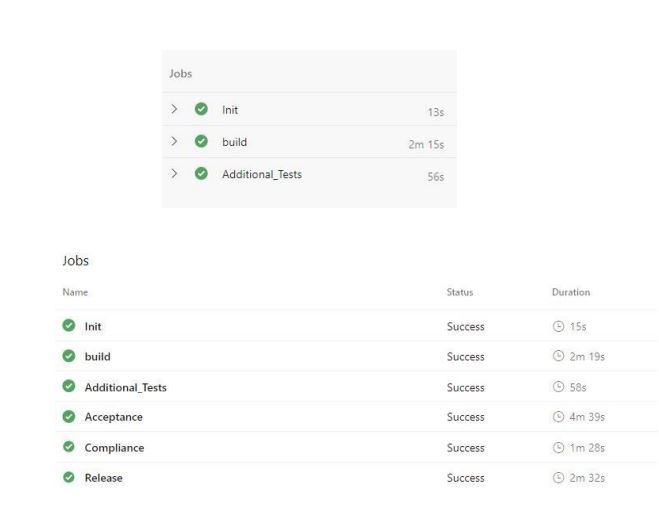
\includegraphics{A_RiskService}}
		\caption[]{Integration- und Delivery-Zeit für den RiskService mit Azure Pipelines. Eigene Darstellung.}
		\label{fig:AP_Risk}
	\end{figure}
\end{center}

\begin{center}
	\begin{figure}[H]
		\centering
		\scalebox{0.7}{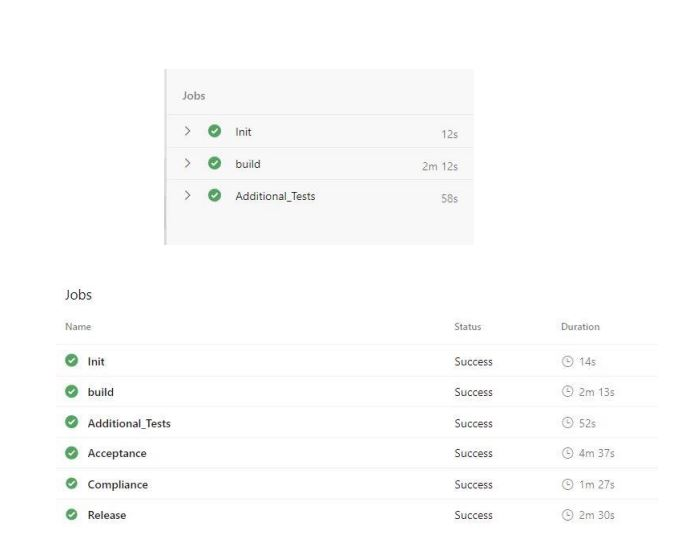
\includegraphics{A_SupplierService}}
		\caption[]{Integration- und Delivery-Zeit für den SupplierService mit Azure Pipelines. Eigene Darstellung.}
		\label{fig:AP_Supplier}
	\end{figure}
\end{center}
\begin{center}
	\begin{figure}[H]
		\centering
		\scalebox{0.7}{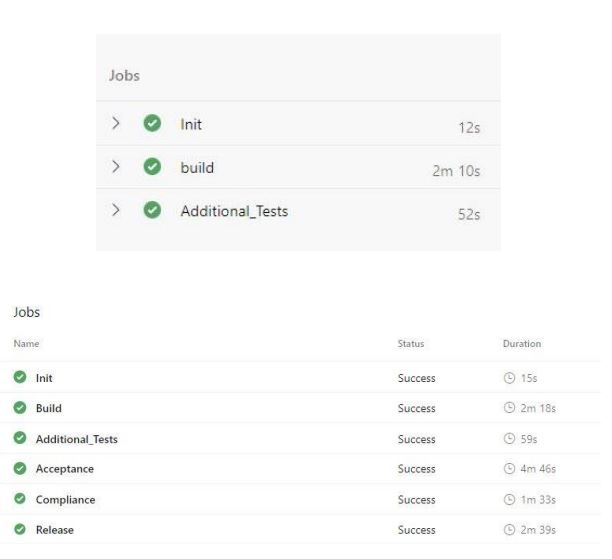
\includegraphics{A_PlantService}}
		\caption[]{Integration- und Delivery-Zeit für den PlantService mit Azure Pipelines. Eigene Darstellung.}
		\label{fig:AP_Plant}
	\end{figure}
\end{center}
                 
\subsection{Jenkins}
\subsubsection{CI-Pipeline-Implementation}
Die Pipeline-Implementation ist bei allen Services identisch:\\
\begin{lstlisting}[language=Python, breaklines=true, basicstyle=\small\ttfamily, frame=single]
@Library('piper-lib-os') _

node() {
    stage('Prepare') {
        deleteDir()
        checkout scm
        setupCommonPipelineEnvironment script:this
    }
	
  stage('Build')   {
      npmExecuteScripts script: this, runScripts: ["initlint"]
      mtaBuild script:this  
  }

  stage('Additional_Tests'){
      npmExecute script: this, dockerImage: (dockerImage), npmCommand : "run mykarma:ci"
    }
}
        \end{lstlisting}



\subsubsection{CD-Pipeline-Implementation}
Die Pipeline-Implementation ist bei allen Services identisch:\\
\begin{lstlisting}[language=Python, breaklines=true, basicstyle=\small\ttfamily, frame=single]


    @Library('piper-lib-os') _

    node() {
        stage('Prepare') {
            deleteDir()
            checkout scm
            setupCommonPipelineEnvironment script:this
        }
        
      stage('Build')   {
          npmExecuteScripts script: this, runScripts: ["initlint"]
          mtaBuild script:this  
      }
    
      stage('Additional_Tests'){
          npmExecute script: this, dockerImage: (dockerImage), npmCommand : "run mykarma:ci"
        }
    
      stage('Acceptance') {
         cloudFoundryDeploy script: this
         uiVeri5ExecuteTests script: this
        }
        
      stage('Compliance') {
         sonarExecuteScan script:this, branchName: "main", githubToken: (githubToken), token:(Token), serverUrl: (serverUrl)
        }
        
        stage('Deploy')   {
         cloudFoundryDeploy script:this
      }
    }
    
        \end{lstlisting}
\subsubsection{Performance-Ergebnisse}

\begin{center}
	\begin{figure}[H]
		\centering
		\scalebox{0.7}{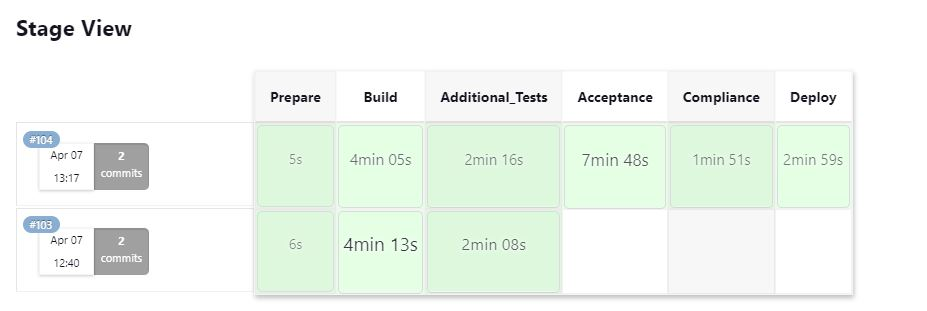
\includegraphics{J_RiskService}}
		\caption[]{Integration- und Delivery-Zeit für den RiskService mit Jenkins. Eigene Darstellung.}
		\label{fig:JP_Risk}
	\end{figure}
\end{center}

\begin{center}
	\begin{figure}[H]
		\centering
		\scalebox{0.7}{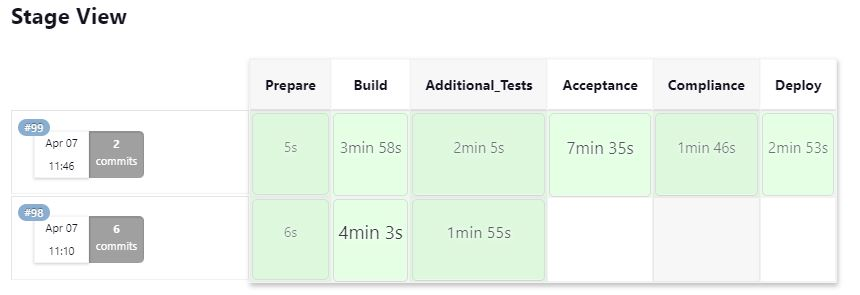
\includegraphics{J_SupplierService}}
		\caption[]{Integration- und Delivery-Zeit für den SupplierService mit Jenkins. Eigene Darstellung.}
		\label{fig:JP_Supplier}
	\end{figure}
\end{center}
\begin{center}
	\begin{figure}[H]
		\centering
		\scalebox{0.7}{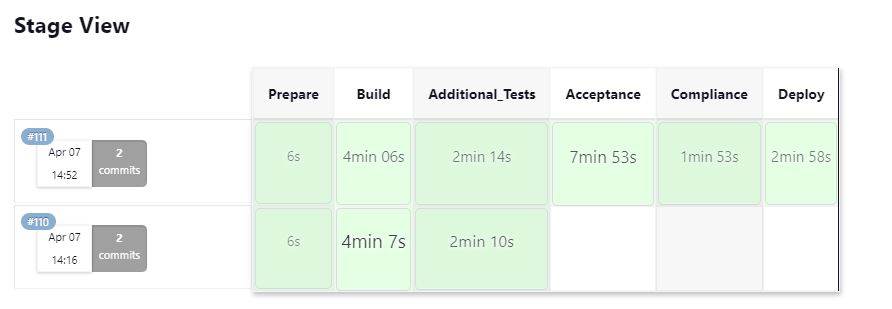
\includegraphics{J_PlantService}}
		\caption[]{Integration- und Delivery-Zeit für den PlantService mit Jenkins. Eigene Darstellung.}
		\label{fig:JP_Plant}
	\end{figure}
\end{center}

\subsection{SAP CI/CD}
\subsubsection{CI-Pipeline-Konfiguration}

\begin{center}
	\begin{figure}[H]
		\centering
		\scalebox{1}{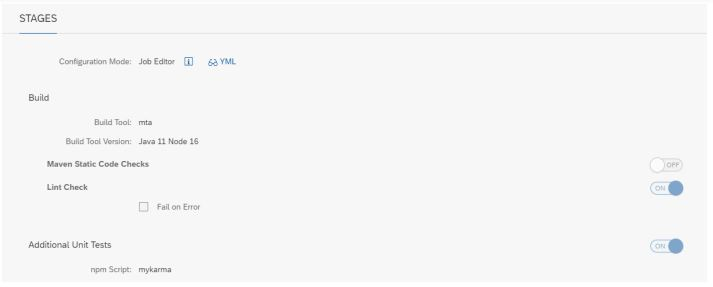
\includegraphics{p_impl_ci}}
		\caption[]{CI-Pipeline-Konfiguration für SAP CI/CD }
		\label{fig:S_IMPl}
	\end{figure}
\end{center}

\subsubsection{CD-Pipeline-Konfiguration}

\begin{center}
	\begin{figure}[H]
		\centering
		\scalebox{1}{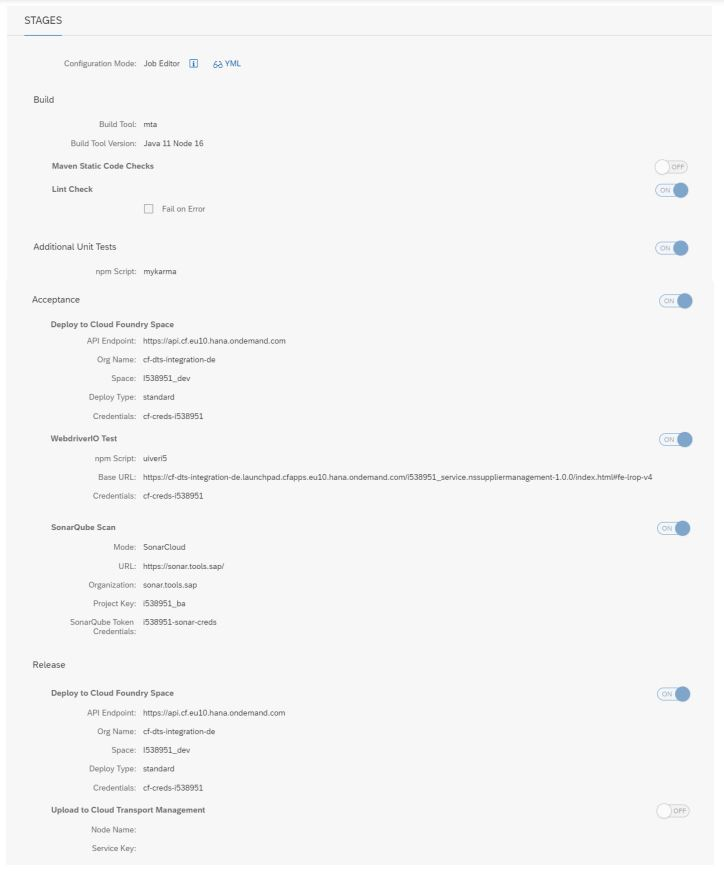
\includegraphics{P_Impl}}
		\caption[]{CD-Pipeline-Konfiguration für SAP CI/CD }
		\label{fig:S_IMPl_CD}
	\end{figure}
\end{center}

\subsubsection{Performance-Ergebnisse}

\begin{center}
	\begin{figure}[H]
		\centering
		\scalebox{1}{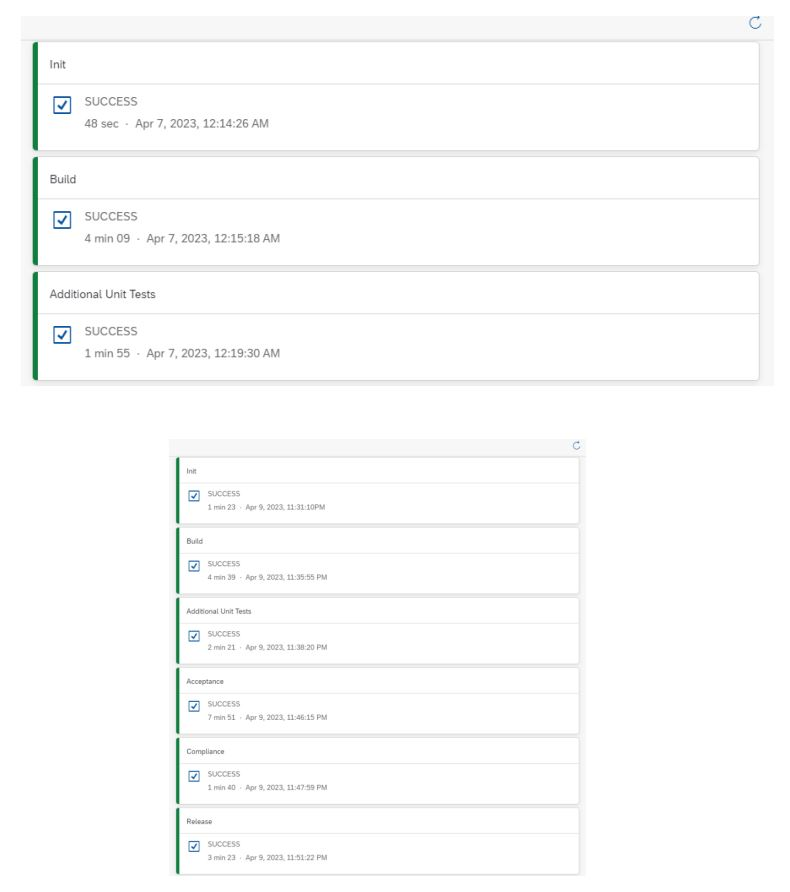
\includegraphics{S_RiskService}}
		\caption[]{Integration- und Delivery-Zeit für den RiskService mit SAP CI/CD. Eigene Darstellung.}
		\label{fig:SP_Risk}
	\end{figure}
\end{center}

\begin{center}
	\begin{figure}[H]
		\centering
		\scalebox{1}{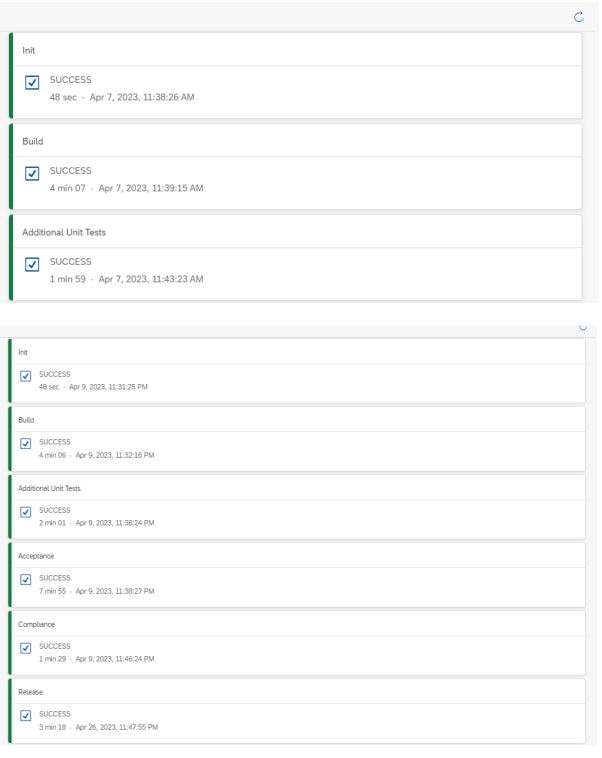
\includegraphics{S_SupplierService}}
		\caption[]{Integration- und Delivery-Zeit für den SupplierService mit SAP CI/CD. Eigene Darstellung.}
		\label{fig:SP_Supplier}
	\end{figure}
\end{center}
\begin{center}
	\begin{figure}[H]
		\centering
		\scalebox{1}{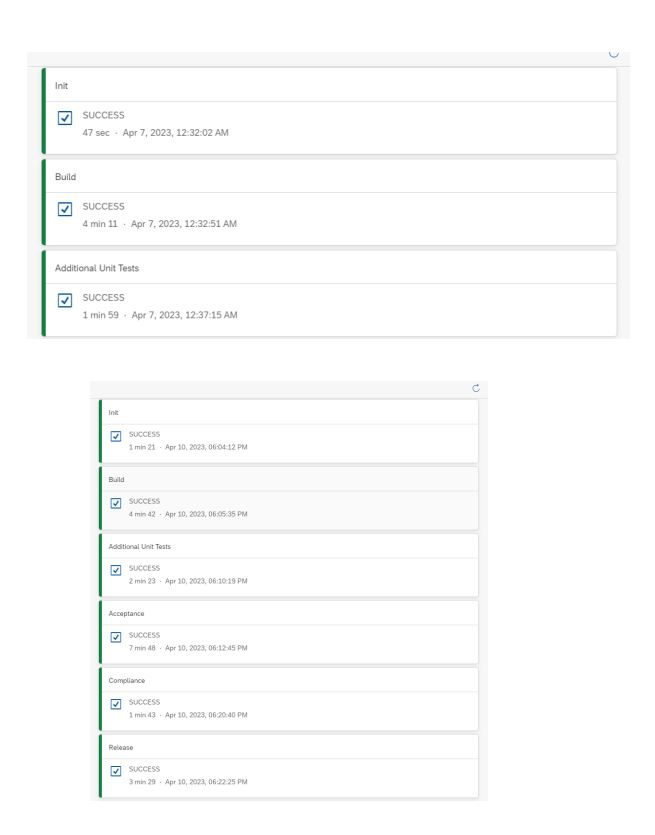
\includegraphics{S_PlantService}}
		\caption[]{Integration- und Delivery-Zeit für den PlantService mit SAP CI/CD. Eigene Darstellung.}
		\label{fig:SP_Plant}
	\end{figure}
\end{center}




\newpage
\section{Expertenmaterialien}
\label{sec:Expertenmaterialien}

\subsection{Experteninterview 1}
	\begin{tabular}{ l l }
		Interviewpartner: & Product Owner SAP BTP Prod\&Infra (Experte 1)\\
		Datum: & 17.03.2023\\
		Interview-Medium: & Microsoft-Teams\\
\end{tabular}\\\\

\begin{linenumbers}
\textbf{Interviewer:} Du kannst dich ja mal kurz vorstellen und erläutern, was du bereits mit dem CI/CD-Bereich zu tun hattest und was deine täglichen Aufgaben sind.\\
\textbf{Experte:} Ich bin Product Owner für den Continuous Integration and Delivery Service. Meine tägliche Aufgabe ist die Steuerung des Backlogs für unsere Anforderungen. Dabei muss ich die Anforderungen, die über verschiedene Kanäle von unseren Kunden hereinkommen konsolidieren und für unsere Abteilung bereitstellen.\\
\textbf{Interviewer:} Wie definierst du den Begriff CI/CD?\\
\textbf{Experte:} Also für mich gibt es einmal den CI Begriff. Dabei habe ich einen CI-Server, der mir nach einem Push in mein zentrales Repository innerhalb kurzer Zeit ein Feedback gibt. Danach kommt der CD-Prozess. Dabei kann ich abhängig von verschiedenen Mechanismen, wie zum Beispiel einem Review oder einem Request die CD-Pipeline auslösen. Die ist i.d.R. auch mächtiger als die CI-Pipeline. Mit dieser wird zentral gebaut, getestet und ggf. auch noch Sachen wie Compliance, Vulnerabilities, statische Codechecks, Integrations-Tests und Performance-Tests abgewickelt. Das getestete Programm kann dann anschließend z.B. in ein Artefakt-Repository oder in eine Produktionsumgebung bereitgestellt werden.\\
\textbf{Interviewer:} Welche Vorteile hat es, wenn Software kontinuierlich bereitgestellt wird?\\
\textbf{Experte:} Der Vorteil ist der, dass ich meine Änderungen in kleinen Paketen, die sich auch leichter integrieren lassen, vollziehe. Wenn ich tägliche oder alle zwei bis drei Tage Änderungen mache und dann jeweils schaue, ob der Status noch grün ist, birgt das gegenüber dem klassischen Wasserfallmodell sehr viele Vorteile. So kann ich, wenn ich schnell in eine Canary-Umgebung bereitstelle, natürlich auch früher Fehler finden, was dann im Endeffekt auch deutlich günstiger wird.\\
\textbf{Interviewer:} Welche unterschiedlichen Arten von Pipelines gibt es?\\
\textbf{Experte:} Das hängt ein wenig von den Anforderungen ab. Also typischerweise hat man eine sehr kleine Pipeline für Request-Votes. Diese wird automatisch ausgelöst, wenn in dem Github ein Pull-Request aufgemacht wird. Diese sollte maximal 10 bis 15 Minuten Laufzeit besitzen. So soll der Entwickler ein schnelles Feedback bekommen. Dann gibt es noch die Delivery-Pipelines. Diese wird dazu verwendet, um in ein Artefakt-Repository oder auf die Produktionsumgebung bereitzustellen. Für solche Pipelines kann entschieden werden, ob entweder alles am Stück gemacht wird oder ob Komponenten aufgeteilt werden. Es bietet sich z.B. an, dass zu Beginn einfache Unit- und Code-Tests gemacht werden und das Artefakt anschließend in das Repository bereitgestellt wird. Konkurrent kann ebenfalls ein Job eingestellt werden, welcher zu einem bestimmten Zeitpunkt durchläuft und ebenfalls aufwändigere Tests abwickelt.\\
\textbf{Interviewer:} Du hattest Artefakt-Repository genannt. Welche Vorteile hat das Artefakt-Repository?\\
\textbf{Experte:} Das spielt insbesondere bei einer CEA eine wichtige Rolle. Kleine entwickelte Komponenten können mit Versionierung in das Artefakt-Repository bereitgestellt werden. Andere Entwickler können diese Komponente dann aus dem Artefakt-Repository herausziehen und für eigenen Entwicklungen wiederverwenden.\\
\textbf{Interviewer:} Welche Stages hat eine typische CI/CD-Pipeline?\\ 
\textbf{Experte:} Typischerweise beginnt eine CI/CD-Pipeline mit dem Build-Stage bei welcher Unit-Tests ausgeführt werden. Für CAP werden dabei die Frameworks Mocha oder Jest verwendet. Dann gibt es eine Acceptance-Stage in welcher Akzeptanztests ausgeführt werden. Solche Akzeptanztests können dann z.B. Integration-Tests umfassen, welche bei CAP-Node-Anwendungen mit Newmann automatisiert werden. Dann gibt es eine Compliance-Stage. In dieser laufen Tools wie die SonarQube. Dort wird z.B. geprüft, ob irgendwelche Lizenzrechte im Code verletzt werden. Anschließend kommt die Security-Stage. In dieser wird nach Vulnerabilities und statischen Kontexten geprüft und evaluiert, ob Gefahr für Cross-Skripting, Null-Pointer-Exceptions etc. besteht. Dann gibt es noch die Release-Stage. Dort wird die Anwendung dann tatsächlich auf die Cloud-Plattform bereitgestellt.\\
\textbf{Interviewer:} Welche Pipelines werden bei der SAP verwendet?\\
\textbf{Experte:} Zum einen wird der von der SAP bereitgestellte CI/CD-Service verwendet. Dieser sollte aber lediglich von Kunden verwendet werden. Dieser eignet sich insbesondere bei weniger komplexen Anwendungen. Des Weiteren gibt es Jenkins. Diese wird i.d.R. mit Project Piper verwendet. Die Jenkins-Pipeline muss dabei selbst gehostet werden. Für interne Projekte wird dafür das Jenkins-as-a-Service angeboten. Häufig wird für interne Projekte ebenfalls Azure Pipelines verwendet.\\
\textbf{Interviewer:} Welche Aspekte sind bei der Wahl eines CI/CD-Pipeline-Tools zu beachten?\\
\textbf{Experte:} Zum einen wie viel Wissen ein Team bereits im DevOps besitzt. Dabei sollte evaluiert werden, ob das Team bereits DevOps-Spezialisten besitzt, welche schon häufig Pipelines implementiert haben. Für Abteilungen, welche keine DevOps-Spezialisten haben, spielt die Benutzerfreundlichkeit eine große Rolle. Da ist es zum einen wichtig, wie leicht sich die Tools warten lassen, aber auch, wie leicht sich eine Pipeline implementieren lässt. Weiterhin ist wichtig zu wissen, wie flexibel man bei der Pipeline-Gestaltung sein will. Zudem muss natürlich auch evaluiert werden, welche Funktionalitäten, also Tests, Code-Scans und Builds auf der Pipeline ausgeführt werden sollen. In Bezug auf die Funktionalität sollte ebenfalls evaluiert werden, auf welcher Plattform die Software bereitgestellt werden soll. Insbesondere für CEA spielt ebenfalls die Skalierbarkeit eine wichtige Rolle. Horizontale Skalierbarkeit umschreibt in diesem Kontext, dass mehrere Build gleichzeitig durchgeführt werden können. Die vertikale Skalierbarkeit bedeutet, dass die Ressourcen einer Pipeline-Instanz flexibel angepasst werden können. Da Jenkins selbst gehostet wird, hat das natürlich für die vertikale Skalierbarkeit einen erheblichen Nachteil. Für viele Kunden spielt ebenfalls die Sicherheit eine ausschlaggebende Rolle. Ein sicheres System ist essenziell, damit in die Produktionsumgebungen keine Maleware eingeschleust werden kann.\\ 
\textbf{Interviewer:} Wie sieht es mit der Unterstützung von Tests aus?\\
\textbf{Experte:} Es ist eigentlich fast alles auf dem SAP BTP CI/CD-Service möglich. Was bisher noch nicht wirklich unterstützt wird, sind API-Tests.\\
\textbf{Interviewer:} Wie sieht es mit den Integrationsmöglichkeiten aus. Worauf muss dabei geachtet werden?\\
\textbf{Experte:} Die Integration ist ebenfalls ein sehr wichtiger Aspekt bei der Auswahl einer CI/CD-Pipeline. Dabei muss darauf geachtet werden, dass die Pipeline mit dem Repository integrierbar ist. Der SAP CI/CD-Service unterstützt einen ganz normalen Git-Server. Was ebenfalls funktioniert, sind BitBucket Repositorys. Für die Integration wird dabei jedoch eine Webhook benötigt. Hierbei können jedoch ausschließlich Commit Events verarbeitet werden. Sehr selten wird eine CI/CD-Pipeline auch in die Entwicklungsumgebung integriert. Das ist mit dem SAP CI/CD-Service nicht möglich. SAP CI/CD hat diese Möglichkeit nicht. Jenkins und Azure können dabei sowohl in Eclipse als auch VSCode eingebunden werden.\\
\textbf{Interviewer:} Gibt es irgendwelche Einschränkungen bezüglich der Laufzeitumgebung?\\
\textbf{Experte:} Bei unserem Service nicht. Wir können sowohl auf Cloud Foundry als auch auf Kyma deployen.\\
\textbf{Interviewer:} Gibt es in dem SAP CI/CD-Tool irgendwelche Überwachungsfun\-ktionalitäten?\\ 
\textbf{Experte:} Für das SAP CI/CD können ausschließlich Pipeline-Logs ausgegeben werden. Da gibt es verschiedene Notification-Services, die über den Erfolg der Pipeline-Builds benachrichtigen. Aber ein direktes Monitoring der Pipeline gibt es nicht.\\
\textbf{Interviewer:} Welche Kosten fallen für die CI/CD-Pipeline an?\\
\textbf{Experte:} Eine Build-Hour kostet einen Euro.\\
\textbf{Interviewer:} Sind parallele Builds möglich und ist die Pipeline mit dem Transport Management System integrierbar?\\
\textbf{Experte:} Nein leider nicht. Aber die Pipeline kann Software auf das Transport Management System bereitstellen.\\
\textbf{Interviewer:} Welche Support-Möglichkeiten stehen für SAP CI/CD bereit?\\
\textbf{Experte:} Wir bieten wie andere SAP-Cloud-Dienste ein Ticket-System mit Service Now an. Wenn Kunden konkrete technische Unterstützung benötigen, können sich diese an die technischen Berater der SAP wenden.\\
\end{linenumbers}
\newpage
\resetlinenumber
\subsection{Experteninterview 2}
	\begin{tabular}{ l l }
		Interviewpartner: & Product Manager SAP Hyperspace CI/CD (Experte 2)\\
		Datum: & 24.03.2023\\
		Interview-Medium: & Microsoft-Teams\\
\end{tabular}\\\\
\begin{linenumbers}
    \textbf{Interviewer:} Du kannst dich nun gerne vorstellen. Wie kommst du während deiner Arbeit mit CI/CD in Berührung?\\
    \textbf{Experte:} Ich bin Product Manager. Ich habe zuerst für den SAP CI/CD-Service gearbeitet. Nun bin ich im Hyperspace.\\
    \textbf{Interviewer:} Was bedeutet für dich CI/CD?\\
    \textbf{Experte:} CI ist die Integration, bei welchem die Änderungen von unterschiedlichen Entwicklern so schnell wie möglich ein zentrales Repository integriert werden. CD ist Continuous Delivery. Das ist die Möglichkeit, ein Feature so schnell wie möglich auf die Produktion zu überführen und für den Kunden bereitzustellen.\\
    \textbf{Interviewer:} Welchen Vorteil hat es Software schnell bereitzustellen?\\
    \textbf{Experte:} Der Vorteil für mich ist, dass man mit kleineren Paketen arbeitet. So ist die Gefahr, dass etwas im Produktivsystem kaputtgeht sehr gering. Mit kleinen Änderungen sind die Auswirkungen, die eine Integration hat, auch besser zu überblicken.\\
    \textbf{Interviewer:} Aus welchen typischen Komponenten besteht eine gewöhnliche Pipeline?\\
    \textbf{Experte:} Also man fängt typischerweise mit dem Sync auf seinem Git Repository an. Der zweite Schritt ist dann der Build. Dort werden auch Unit-, Integration- und Acceptance-Tests in unterschiedlichen Spaces ausgeführt. In einer Acceptance-Stage werden dann mehr Tests als in der Build-Phase durchgeführt. Dazu gehören neben normalen Tests auch Security-Scans. Zuletzt wird die Software bereitgestellt.\\
    \textbf{Interviewer:} Wie sind Pipelines aufgebaut?\\
    \textbf{Experte:} Also früher haben wir keine unterschiedlichen Pipelines für CI und CD verwendet. Da haben wir aber gesehen, dass das ziemlich problematisch ist. Wenn alles sequenziell ausgeführt wird und dann in der Mitte irgendwas abbricht, ist mit diesem Vorgehen sehr viel Zeit verloren gegangen. Nun geht der Trend in Richtung Shift-Left. Die Pipelines werden somit deutlich verkleinert, womit schnelleres Feedback gegeben werden kann.\\
    \textbf{Interviewer:} Welche Kriterien sollten bei der Auswahl von Pipelines beachtet werden.\\
    \textbf{Experte:} Es kommt natürlich darauf an, welche Produktstandards vorgegeben sind. Wenn die Standards hoch sind, ist auch die Test-Funktionalität sehr wichtig. Dazu gehören insbesondere Security-Checks, wie mit Fortify. Für sehr großen Entwicklungsprojekte ist es ebenfalls essenziell, dass die Pipelines eine gute Performance besitzen. Somit kann Software schneller bereitgestellt werden. Des Weiteren ist es essenziell, dass die CI/CD-Prozesse überwacht werden können. Gerade bei komplexen Systemen mit vielen Services ist das für den DevOps-Engineer oft die einzige Möglichkeit, die Prozesse nachhaltig zu überblicken. Dann ist natürlich auch wichtig, wie gut sich die Pipeline in die Infrastruktur integrieren lässt. Bei dieser Integration sollten jedoch jegliche Sicherheitsstandards eingehalten werden. Insbesondere für kleinere Kunden ist es essenziell, welche Kosten durch die Pipeline verursacht werden. Für viele Kunden ist darüber hinaus der Support wichtig. Es sollten kontinuierliche Updates, Schulungsmaterial sowie wie eine gute Dokumentation verfügbar sein. Außerdem ist es für Entwickler immer vorteilhaft, wenn für die Tools eine große Community existiert.\\
    \textbf{Interviewer:} Mit welchen Pipelines hattest du bisher Erfahrung?\\
    \textbf{Experte:} Mit Azure DevOps habe ich bisher noch nicht so viel Erfahrung gemacht. In meinem jetzigen Team arbeite ich mit dem Jenkins-as-a-Service. In meinem vorherigen Team habe ich Erfahrung mit dem SAP CI/CD-Service gemacht. Ursprünglich wurde das Projekt Piper für Jenkins nur für interne Projekte genutzt. Mittlerweile wurde die Bibliothek als Open-Source veröffentlicht. Für interne Projekte darf das SAP CI/CD aufgrund der derzeitigen Produktstandards nicht verwendet werden. Dieser wird eigentlich nur für Kunden angeboten. Das SAP CI/CD-Tool lohnt sich insbesondere für Kunden, welche noch nicht viel DevOps-Expertise besitzen und auch keine teure Infrastruktur betreiben wollen.\\
    \textbf{Interviewer:} Ist in dem CI/CD-Service von der SAP schon der Preis für Tools wie SonarQube einberechnet?\\
    \textbf{Experte:} Nein, der Preis ist nicht einberechnet. Tools wie SonarQube müssen von den Kunden selbst gehostet werden.\\
    \textbf{Interviewer:} Weißt du, ob die Tools in das SAP CTM integrierbar sind?\\
    \textbf{Experte:} Ja, sowohl JaaS als auch SAP BTP CI/CD sind in das SAP CTM integrierbar. Intern habe ich noch nicht oft gehört, dass dieser verwendet wird. Aber Kunden können theoretisch auf das SAP CTM bereitstellen. Das SAP CTM ist ebenfalls mit einem Change Management Surface verbunden. Damit kann man einen Change-Auftrag erstellen und Artefakte zwischen unterschiedlichen Systemen bereitstellen. Dadurch hat man einfach mehr Transparenz. Außerdem bietet das System für Composable-ERP-Systeme einen großen Vorteil. Über das SAP CTM können Abhängigkeiten zwischen verschiedenen Microservices definiert werden.\\
    \textbf{Interviewer:} Welche Überwachungsfunktionalitäten bieten die Pipelines und welche Tools werden von Kunden i.d.R. verwendet?\\
    \textbf{Experte:} Bei Jenkins weiß ich, dass man Logs auslesen und den Workflow somit nachvollziehen kann. Für Monitoring wird innerhalb der SAP i.d.R. das SAP-Partner-Tool Splunk verwendet. Das ist über Project Piper einbindbar. Kunden nutzen häufig auch andere Open-Source-Tools. Ein sehr häufig verwendetes Tool ist dabei das Kibana-Dasboard.
\end{linenumbers}
\newpage
\resetlinenumber
\subsection{Experteninterview 3}
	\begin{tabular}{ l l }
		Interviewpartner: & Product Manager SAP Hyperspace Security Tools (Experte 3)\\
		Datum: & 22.03.2023\\
		Interview-Medium: & Microsoft-Teams\\
\end{tabular}\\\\

\begin{linenumbers}
    \textbf{Interviewer:} Wie hat sich das Thema Security im CI/CD-Kontext verändert?\\
    \textbf{Experte:} In letzter Zeit hat sich das Thema Shift Left sehr stark etabliert. Das bedeutet, dass das Feedback eigentlich möglichst früh an den Entwickler zurückgegeben wird. Der Entwickler lernt somit viel nachhaltiger, da er im Integration-Kontext noch keine große Verantwortung hat und somit kleine Arbeitspakete zur Verfügung gestellt bekommt. Falls hingegen große Pakete in die Main-Line integriert werden, ist irgendwann nicht mehr ersichtlich, wer welche Änderungen gemacht hat. Früher gab es dabei immer einen Security-Experten, welcher sich vor der Auslieferung um alles kümmern musste.\\
    \textbf{Interviewer:} Wie wird Security in DevOps heutzutage gemacht?\\
    \textbf{Experte:} Security sollte nicht mehr nur von einem Spezialisten behandelt werden. Vielmehr sollte dies als Kollektiv vorangetrieben werden. Jeder muss bei der Entwicklung seiner Funktionalitäten schon so früh wie möglich schauen, ob alle sicherheitsrelevanten Aspekte eingehalten wurden. Das wird dann i.d.R. durch Automatisierung gemacht. Es wird dabei schon sehr lange mit Security-Tools gearbeitet. Historische Tools sind dabei aber nicht sehr benutzerfreundlich. D.h., dass die Findings nicht gut präsentiert werden. Somit versteht ein normaler Entwickler nicht, was mit einem Finding gemeint ist und wie dieses Problem behoben werden kann. Da haben sich in der letzten Zeit aber sehr viele neue und benutzerfreundlichere Tools etabliert. Diese sollen bei der Realisierung des Shift-Left-Ansatzes unterstützen. Gerade bei der Bereitstellung von ERP-Funktionalitäten sind Security-Scans sehr wichtig. Bei der SAP gelten hierfür sehr strikte Produktstandards. Diese Security-Scans können dabei sehr komplex sein. So ist es die Regel, dass ein Testdurchlauf auch mal mehr als fünf Stunden Zeit in Anspruch nimmt.\\
    \textbf{Interviewer:} Welche Arten von Security-Tools gibt es?\\
    \textbf{Experte:} Es gibt i.d.R. zwei verschiedene Arten von Security-Tools. Es gibt da zum einen die statischen Code-Analysen (SAST). Dort wird insbesondere OS-Scanning betrieben. Dann gibt es noch das Dynamic Application Security Testing (DAST). Dort werden dann auch tatsächlich UI-Elemente, APIs sowie Datenbanken gescannt. Damit können im Produktionssystem leichter Scripting-Attacken oder SQL-Injections verhindert werden. Manchmal wird dann auch noch die Kategorie des Interactive Application Security Testing (IAST) definiert. Dabei wird ein Agent in die Laufzeitumgebung integriert, welcher die Insights der Analysen liefert. Dort können dann z.B. Software-Component-Analysen gemacht werden, bei welchen HTTP-Requests gespooft werden.\\
    \textbf{Interviewer:} Welche Tools werden bei der SAP mit Project Piper verwendet?\\
    \textbf{Experte:} Zum einen gibt es Fortify. Das ist insbesondere für Java und Python. Das Tool ist allerdings kaum noch in Verwendung, da es sich historisch nicht weiterentwickelt hat. In näherer Zukunft wird dieses durch GitHub Advanced Security abgelöst. Für CAP Node wird in den Produktstandards das Tool Checkmarx vorgeschrieben. Für Open-Source ist das Tool Whitesource vorgeschrieben. Für SAP UI5 wird bei der statischen Code-Analyse Checkmarx verwendet. Für Open-Source gibt es keine Vorgabe. Das liegt daran, dass UI5 eigentlich über JavaScript geschrieben wird und somit NPM als Package-Manager benötigt. Node wird in dieser Technologie jedoch nicht unterstützt. Für statische Codeanalysen wird SonarQube und Lint verwendet.
\end{linenumbers}

\newpage
\resetlinenumber
\subsection{Experteninterview 4}
	\begin{tabular}{ l l }
		Interviewpartner: & Frontend-Test-Entwickler SAP Hyperspace (Experte 4)\\
		Datum: & 22.03.2023\\
		Interview-Medium: & Microsoft-Teams\\
\end{tabular}\\\\

\begin{linenumbers}
    \textbf{Interviewer:} Du kannst dich nun gerne vorstellen.\\
    \textbf{Experte:} Derzeit bin ich im Adoption and Onboarding Team von Hyperspace. Wir unterstützen Kunden darin, ihre Projekte zu onboarden. Dafür bieten wird verschiedene Toolings, wie Security-Tools, Deployment-Tools, Test-Tools etc. an.\\
    \textbf{Interviewer:} Was hat das Hyperspace mit CI/CD zu tun?\\
    \textbf{Experte:} Hyperspace ist eine Plattform, die es ermöglicht, das CI/CD-Set-up mög\\lichst konsistent und einfach aufzusetzen. Somit soll der kognitive Load in den Teams reduziert werden, um nicht alles manuell aufsetzen zu müssen. Gerade das Aufsetzen einer Pipeline mit Jenkins, bei welchem u.a. auch Groovy-Scripten usw. benötigt werden, kann einen sehr hohen Aufwand darstellen. Zudem benötigt dies sehr viel Wissen. Hyperspace gibt den Entwicklungsteams Guidelines vor. D.h. auf Hyperspace kann ich einfach ein Template auswählen. Das Hyperspace kümmert sich dann darum, dass alle benötigten Tools zur Verfügung stehen und nicht alles selbst konfiguriert werden muss.\\
    \textbf{Interviewer:} Wird im Hyperspace auch eine konkrete Step-Implementierung abgenommen?\\
    \textbf{Experte:}  Hyperspace erzeugt einem eigentlich erst mal so eine Ready-Made-Pipeline. Das ist eine standardisierte Vorgabe, auf welcher man dann Konfigurationen vornimmt. Dann kannst du z.B. einstellen, welche Tools du verwenden möchtest. Du kannst natürlich davon ausbrechen und sagen okay, ich möchte da jetzt einen kompletten Step überschreiben etc. Das Ziel ist jedoch den kognitiven Load so gering wie möglich zu halten.\\
    \textbf{Interviewer:} Wie definierst du für dich CI/CD?\\
    \textbf{Experte:} Ich bin dort jetzt kein kompletter Experte, aber mein Hauptmotiv als Entwickler ist, es möglichst schnelles Feedback zubekommen. Früher war es so, dass ich Tests geschrieben habe und die dann einmal in der Woche ausgeführt habe. Aufgrund der Verzögerung ist das natürlich nicht besonders geschickt. Bei einem guten Setup mache ich eine Änderung und bekomme beim Commit direkt ein Feedback. Das zweite ist natürlich, dass ich neue Produktversionen sehr schnell zum Kunden bekomme. Idealerweise innerhalb von einer Woche oder vielleicht sogar manchmal in einem Tag. Als ich damals in einer SAP-Partnerfirma war, haben wir manchmal ein ganzes Jahr entwickelt. Dann gab es eine sehr große Testphase. Und am Ende hat sich herausgestellt, dass der Kunde etwas ganz anderes haben wollte.\\
    \textbf{Interviewer:} Welchen Vorteil hat es, wenn man den CI/CD-Prozess automatisiert?\\
    \textbf{Experte:} Man hat die Möglichkeit, neue Features erst mal einzelnen Kunden bereitzustellen. Wenn ich dann feststelle, dass irgendwas nicht funktioniert, kann ich schnell ein Rollback machen. Des Weiteren gibt es dann z.B. das Feature-Toggle. Da wird eine neue Funktionalität dann hinter einer Flag versteckt. Wenn ein bestimmter Kunde dieses Feature haben möchte, dann setzt er entsprechend die Flag.\\
    \textbf{Interviewer:} Welche Art von Pipelines werden denn i.d.R. verwendet?\\
    \textbf{Experte:} Ich kenne hauptsächlich die Pull-Request-Pipeline. Häufig gibt es dann auch noch einmal eine Pipeline, welche einmal am Tag läuft, bei welcher dann Tests gemacht werden, welche deutlich länger laufen.\\
    \textbf{Interviewer:} Welchen Vorteil hat ein Artefakt-Repository?\\
    \textbf{Experte:} Das Artefakt-Repository wird verwendet, um das Coding was erzeugt wurde, versioniert abzulegen. Dieses wird dann in der Pipeline immer wieder verwendet, um z.B. Tests dagegen auszuführen. Mit diesen Artefakten kann man dann auch noch sehr gut Rollbacks ausführen. Das heißt, wenn man merkt, dass eine neue Version nicht funktioniert, kann man einfach wieder zur alten Version zurückspringen.\\
    \textbf{Interviewer:} Welche Pipelines werden bei der SAP im Regelfall verwendet?\\
    \textbf{Experte:} Auf der Orchestratorseite ist es so, dass ganz viel über Azure Pipelines gemacht wird. Diese bietet z.B. einige Governace-Checks an, was sich gerade in der Standardentwicklung als Vorteil erweist. Außerdem ist der Wartungsaufwand einfach viel geringer. Das SAP Tools Team hat  alles auf einen zentralen Blick und kann entsprechend sehen, ob einer Pipeline irgendwie mehr Ressourcen zugewiesen werden müssen. Zudem bekommt die SAP, weil sie Microsoft-Partner ist, auch gute Konditionen bei dieser Firma. Ein weiterer Vorteil von Azure Pipelines sind Mechanismen, wie Caching oder Parallel Builds. In der internen Standardentwicklung haben diese dafür gesorgt, dass die CI/CD-Prozesse um 35 Prozent beschleunigt wurden. Bei Azure Pipelines werden zudem sehr viele Technologien unterstützt, was insbesondere bei Unternehmen, welche einen hohen Wert auf Technologieoffenheit legen, von Vorteil sein könnte. Für kleinere Teams wie das SAP Sports One empfiehlt sich Azure Pipelines nicht. Diese sollten eher auf Jenkins setzen.\\
    \textbf{Interviewer:} Welche Tests werden bei der SAP gemacht?\\
    \textbf{Experte:} Bei der SAP werden durch den Produktstandard gemäß ISO 9001 verschiedene Validierungen vorgeschrieben. Für Unit Tests gibt es dafür verschiedene Frameworks. I.d.R. wird bei der SAP Q-Unit für Frontend und Mocha oder Jest für das Backend verwendet. Für Q-Unit wird die Laufzeitumgebung Karma und für Mocha und Jest Node benötigt. Für Frontend-Integration-Tests wird OPA5 verwendet. Dafür benötigt es ebenfalls der Laufzeitumgebung Karma. Für Integration-Tests im Backend wird Newmann verwendet. Mit Newman können Postmann-Tests automatisiert werden. Und für E2E-Tests im Frontend wird dann i.d.R. WDI5 verwendet. Damit lassen sich dann ganze Anwenderszenarien testen. Das hat den Vorteil, dass ich wie ein End-User teste. Nachteil ist dabei jedoch, dass ich schauen muss, dass die Daten verfügbar sind, Customizings gemacht wurden etc. Um OPA5 in einer Pipeline zu automatisieren wird die Webdriver.io Laufzeitumgebung benötigt. Alle, die hier genannten Laufzeitumgebungen werden durch das Project Piper ausgeliefert. Aber man muss die Tests natürlich immer gezielt einsetzen. Wir haben damals in unsere Pipeline E2E-Tests eingebaut und dadurch hat die Pipeline um den Faktor 3 länger gebraucht. Noch einmal zur zentralen Aussage der Testpyramide. Die Empfehlung ist, möglichst viel auf den unteren Ebenen abzudecken, also mit Unit-Tests und auf den oberen Ebenen nur noch das zu testen, was man nicht mit Unit- und Integration-Tests validieren kann.\\
    \textbf{Interviewer:} Werden denn immer alle Tests ausgeführt?\\
    \textbf{Experte:} Also bei einer Pull-Request-Pipeline sollten auf jeden Fall die Unit- und Integration-Tests laufen. Die System-Tests werden dann z.B. einmal am Tag ausgeführt. Manche Teams verwenden auch eine parallele Ausführung von Tests und führen dann eben verschiedene Szenarien gleichzeitig durch. Das läuft dann i.d.R. schneller und dann können solche Tests auch beim Pull-Request ausgeführt werden. Gerade die Compliance und Accessibility-Tests werden dann eher in der Delivery-Pipeline durchgeführt.\\
    \textbf{Interviewer:} Auf welche Integrationsaspekte muss geachtet werden?\\
    \textbf{Experte:} In den bisherigen Projekten, in welchen ich gearbeitet habe, wurde die Auswahl einer CI/CD-Pipeline immer sehr stark von dem Repository abhängig gemacht. Die Repositorys, welche von Kunden dabei besonders oft verwendet werden, sind GitHub, GitLab und BitBucket. Was auch, aber eher selten in Kundenprojekten beachtet wird, ist die Integrierbarkeit in Projektmanagement-Tools. Häufig wird dabei Jira verwendet, aber i.d.R. machen die Kunden die Wahl einer CI/CD-Pipeline nicht von der Unterstützung eines spezifischen Tools abhängig. Um einen Überblick über die Bereitstellungsprozesse zu erhalten, müssen Experten somit nicht in den Code schauen, sondern haben alles in einem zentralen Tool. SAP CI/CD unterstützt das nicht, wohingegen ich gehört habe, dass es diese Möglichkeit bei Jenkins sowie Azure Pipelines gibt.\\ 
    \textbf{Interviewer:} Wie wird der Entwickler über den Erfolg der Tests informiert?\\
    \textbf{Experte:} Da gibt es unterschiedliche Verfahrensweisen. Es gibt da dann z.B. verschiedene Monitoring-Tools in der CI/CD-Pipeline. Ein anderer Weg ist, wenn man die CI/CD-Pipeline über APIs in das Repository integriert. Was auch häufig gemacht wird ist, dass man die Pipelines in den SAP Alert Service integriert, sodass Entwickler dann entsprechend Nachrichten über Mail oder Slack bekommen.
\end{linenumbers}

\newpage
\subsection{Kodierung der Experteninterviews}
\label{sec:kodierung}
\underline{Was ist CI/CD?}\\
\begin{longtable}{ |C{6cm}|C{3cm}|c|c| }
	\hline
	Aussage & Kodierung & Experte & Zeilennummer\\
	\hline
	\enquote{Dabei habe ich einen CI-Server, der mir nach einem Push in mein zentrales Repository innerhalb kurzer Zeit ein Feedback gibt.} & CI & Experte 1 & 8 ff. \\
	\hline
	\enquote{Das ist die Möglichkeit, ein Feature so schnell wie möglich auf die Produktion zu überführen und für den Kunden bereitzustellen.} & CD & Experte 2 & 10 ff. \\
	\hline
	\end{longtable}

\underline{Verschiedene Arten von Pipelines}\\
\begin{longtable}{ |C{6cm}|C{3cm}|c|c| }
	\hline
	Aussage & Kodierung & Experte & Zeilennummer\\
	\hline
	\enquote{[Mit der CD-Pipeline] wird zentral gebaut, getestet und ggf. auch noch Sachen wie Compliance, Vulnerabilities, statische Codechecks, Integrations-Tests und Performance-Tests abgewickelt.} & Bestandteile CD-Pipeline  & Experte 1 & 12 ff. \\
	\hline
	\enquote{Diese sollte maximal 10 bis 15 Minuten Laufzeit besitzen. So soll der Entwickler ein schnelles Feedback bekommen.} & Pull-Request-Pipeline & Experte 1 & 28 ff. \\
	\hline
    \enquote{ Die Pipelines werden somit deutlich verkleinert, womit schnelleres Feedback gegeben werden kann.} & Kleine Pipelines & Experte 2 & 29 ff. \\
	\hline
	\end{longtable}



    \underline{Deploy und Release}\\
\begin{longtable}{ |C{6cm}|C{3cm}|c|c| }
	\hline
	Aussage & Kodierung & Experte & Zeilennummer\\
	\hline
	\enquote{Das getestete Programm kann dann anschließend z.B. in ein Artefakt-Repository oder in eine Produktionsumgebung bereitgestellt werden.} & Artefakt-Repository und Produktionsumgebung  & Experte 1 & 15 ff. \\
	\hline
    \enquote{Mit diesen Artefakten kann man dann auch noch sehr gut Rollbacks ausführen.} & Artefakt-Repository  & Experte 4 & 47 ff. \\
	\hline
	\enquote{Kleine entwickelte Komponenten können mit Versionierung in das Artefakt-Repository bereitgestellt werden. Andere Entwickler können diese Komponente dann aus dem Artefakt-Repository herausziehen und für eigenen Entwicklungen wiederverwenden} & Komponentenwiederverwendung im Artefakt-Repository & Experte 1 & 40 ff. \\
	\hline
	\end{longtable}

\newpage
\underline{Test}\\
\begin{longtable}{ |C{6cm}|C{3cm}|c|c| }
    \hline
    Aussage & Kodierung & Experte & Zeilennummer\\
    \hline
    \enquote{Typischerweise beginnt eine CI/CD-Pipeline mit dem Build-Stage bei welcher Unit-Tests ausgeführt werden. Für CAP werden dabei die Frameworks Mocha oder Jest verwendet.} & Unit-Tests mit SAP CAP Node & Experte 1 & 45 ff. \\
    \hline
    \enquote{Solche Akzeptanztests können dann z.B. Integration-Tests umfassen, welche bei CAP-Node-Anwendungen mit Newmann automatisiert werden.} & Integration-Tests mit SAP CAP Node & Experte 1 & 48 ff. \\
    \hline
    \enquote{I.d.R. wird bei der SAP Q-Unit für Frontend und Mocha oder Jest für das Backend verwendet.} & Unit-Tests mit SAP UI5 & Experte 4 & 66 ff. \\
    \hline
    \enquote{Für Integration-Tests wird OPA5 verwendet.} & Integration-Tests mit SAP UI5 & Experte 4 & 69 ff. \\
    \hline
    \enquote{UUnd für E2E-Tests im Frontend wird dann i.d.R. WDI5 verwendet.} & System-Tests mit SAP UI5 & Experte 4 & 72 ff. \\
    \hline
    \enquote{Die Empfehlung ist, möglichst viel auf den unteren Ebenen abzudecken, also mit Unit-Tests und auf den oberen Ebenen nur noch das zu testen, was man nicht mit Unit- und Integration-Tests validieren kann.} & Zeitpunkt für Tests & Experte 4 & 80 ff. \\
    \hline
    \end{longtable}

    \underline{Code-Analysen}\\
\begin{longtable}{ |C{6cm}|C{3cm}|c|c| }
    \hline
    Aussage & Kodierung & Experte & Zeilennummer\\
    \hline
    \enquote{Für statische Codeanalysen wird SonarQube und Lint verwendet.} & Statische Code-Analysen & Experte 3 & 45 ff. \\
    \hline
    \enquote{Für CAP Node wird in den Produktstandards das Tool Checkmarx vorgeschrieben} & SAP CAP Node  & Experte 3 & 40 ff. \\
    \hline
    \enquote{Für SAP UI5 wird bei der statischen Code-Analyse Checkmarx verwendet.} & SAP UI5  & Experte 3 & 41 ff. \\
    \hline
    \end{longtable}
\newpage
    \underline{Vorteile von kontinuierlicher Bereitstellung}\\
    \begin{longtable}{ |C{6cm}|C{3cm}|c|c| }
        \hline
        Aussage & Kodierung & Experte & Zeilennummer\\
        \hline
        \enquote{So kann ich, wenn ich schnell in eine Canary-Umgebung bereitstelle, natürlich auch früher Fehler finden, was dann im Endeffekt auch deutlich günstiger wird.} & Frühe Fehlerfindung & Experte 1 & 23 ff. \\
        \hline
        \enquote{So ist die Gefahr, dass etwas im Produktivsystem kaputtgeht sehr gering.} & Wenig Fehler in der Produktion & Experte 2 & 13 ff. \\
        \hline
        \enquote{Da wird eine neue Funktionalität dann hinter einer Flag versteckt. Wenn ein bestimmter Kunde dieses Feature haben möchte, dann setzt er entsprechend die Flag.} & Feature Toggle & Experte 4 & 37 ff. \\
        \hline
        \end{longtable}




    \underline{CI/CD-Pipeline-Tools bei der SAP}\\
\begin{longtable}{ |C{6cm}|C{3cm}|c|c| }
    \hline
    Aussage & Kodierung & Experte & Zeilennummer\\
    \hline
    \enquote{Zum einen wird der von der SAP bereitgestellte CI/CD-Service verwendet.} & SAP BTP CI/CD & Experte 1 & 57 ff. \\
    \hline
    \enquote{Des Weiteren gibt es Jenkins. Diese wird i.d.R. mit Project Piper verwendet.} & Jenkins & Experte 1 & 59 ff. \\
    \hline
    \enquote{Häufig wird für interne Projekte ebenfalls Azure Pipelines verwendet.} & Azure Pipelines & Experte 1 & 62 ff. \\
    \hline
    \end{longtable}

    \underline{Aspekte für Wahl einer CI/CD-Pipeline}\\
    \begin{longtable}{ |C{6cm}|C{3cm}|c|c| }
        \hline
        Aussage & Kodierung & Experte & Zeilennummer\\
        \hline
        \enquote{Für Abteilungen, welche keine DevOps-Spezialisten haben, spielt die Benutzerfreundlichkeit eine große Rolle. Da ist es zum einen wichtig, wie leicht sich die Tools warten lassen, aber auch, wie leicht sich eine Pipeline implementieren lässt. } & Intuitive Bedienbarkeit und Installation und Wartung & Experte 1 & 67 ff. \\
        \hline
        \enquote{Weiterhin ist wichtig zu wissen, wie flexibel man bei der Pipeline-Gestaltung sein will.} & Flexibilität & Experte 1 & 70 ff. \\
        \hline
        \enquote{Zudem muss natürlich auch evaluiert werden, welche Funktionalitäten, also Tests, Code-Scans und Builds auf der Pipeline ausgeführt werden sollen.} & Tests, Code-Analysen Build & Experte 1 & 71 ff. \\
        \hline
        \enquote{In Bezug auf die Funktionalität sollte ebenfalls evaluiert werden, auf welcher Plattform die Software bereitgestellt werden soll.} & Deploy und Release & Experte 1 & 73 ff. \\
        \hline
        \enquote{Insbesondere für CEA spielt ebenfalls die Skalierbarkeit eine wichtige Rolle.} & Skalierbarkeit & Experte 1 & 74 ff. \\
        \hline
        \enquote{Die Integration ist ebenfalls ein sehr wichtiger Aspekt bei der Auswahl einer CI/CD-Pipeline.} & Integrationsmöglichkeiten & Experte 1 & 88 ff. \\
        \hline
        \enquote{Dabei muss darauf geachtet werden, dass die Pipeline mit dem Repository integrierbar ist.} & Integrationsmöglichkeiten von Repositorys & Experte 1 & 89 ff. \\
        \hline
        \enquote{Sehr selten wird eine CI/CD-Pipeline auch in die Entwicklungsumgebung integriert.} & Integrationsmöglichkeiten von Entwicklungsumgebung & Experte 1 & 93 ff. \\
        \hline
        \enquote{Was auch, aber eher selten in Kundenprojekten beachtet wird, ist die Integrierbarkeit in Projektmanagement-Tools. Häufig wird dabei Jira verwendet, aber i.d.R. machen die Kunden die Wahl einer CI/CD-Pipeline nicht von der Unterstützung eines spezifischen Tools abhängig.} & Integration in Planungstools & Experte 4 & 96 ff. \\
        \hline
        \enquote{Für sehr großen Entwicklungsprojekte ist es ebenfalls essenziell, dass die Pipelines eine gute Performance besitzen. Somit kann Software schneller bereitgestellt werden.} & Performance & Experte 2 & 35 ff. \\
        \hline
        \enquote{Des Weiteren ist es essenziell, dass die CI/CD-Prozesse überwacht werden können. } & Monitoring & Experte 2 & 37 ff. \\
        \hline
        \enquote{Insbesondere für kleinere Kunden ist es essenziell, welche Kosten durch die Pipeline verursacht werden.} & Kosten & Experte 2 & 42 ff. \\
        \hline
        \enquote{Für viele Kunden ist darüber hinaus der Support wichtig. Es sollten kontinuierliche Updates, Schulungsmaterial sowie wie eine gute Dokumentation verfügbar sein.} & Administrativer Support & Experte 2 & 44 ff. \\
        \hline
        \enquote{Außerdem ist es für Entwickler immer vorteilhaft, wenn für die Tools eine große Community existiert.} & Administrativer Support & Experte 2 & 46 ff. \\
        \hline
        \enquote{Für viele Kunden spielt ebenfalls die Sicherheit eine ausschlaggebende Rolle.} & Sicherheit & Experte 1 & 79 ff. \\
        \hline
        
        \end{longtable}

        \underline{SAP BTP CI/CD-Service}\\
\begin{longtable}{ |C{6cm}|C{3cm}|c|c| }
    \hline
    Aussage & Kodierung & Experte & Zeilennummer\\
    \hline
    \enquote{Was bisher noch nicht wirklich unterstützt wird, sind API-Tests.} & Keine API-Tests &Experte 1 & 85 ff. \\
    \hline
    \enquote{Der SAP CI/CD-Service unterstützt einen ganz normalen Git-Server. Was ebenfalls funktioniert, sind BitBucket Repositorys. } & Unterstützung von Repositorys &Experte 1 & 90 ff. \\
    \hline
    \enquote{Hierbei können jedoch ausschließlich Commit Events verarbeitet werden.} & Unterstützung von Commit-Events & Experte 1 & 92 ff. \\
    \hline
    \enquote{Aber ein direktes Monitoring der Pipeline gibt es nicht.} & Kein Monitoring für SAP CI/CD &Experte 1 & 104 ff. \\
    \hline
    \enquote{Eine Build-Hour kostet einen Euro.} & Kosten  &Experte 1 & 106 ff. \\
    \hline
    \enquote{ Wir können sowohl auf Cloud Foundry als auch auf Kyma deployen.} & Deployment  &Experte 1 & 99 ff. \\
    \hline
    \enquote{Nein leider nicht. Aber die Pipeline kann Software auf das Transport Management System bereitstellen.} & Parallel Build und SAP CTM  &Experte 1 & 109 ff. \\
    \hline
    \enquote{Für interne Projekte darf das SAP CI/CD aufgrund der derzeitigen Produktstandards nicht verwendet werden.} & Nicht für interne Projekte  & Experte 2 & 53 ff. \\
    \hline
    \enquote{Das SAP CI/CD-Tool lohnt sich insbesondere für Kunden, welche noch nicht viel DevOps-Expertise besitzen und auch keine teure Infrastruktur betreiben wollen.} & Für Kunden mit wenig Expertise  & Experte 2 & 55 ff. \\
    \hline
    \end{longtable}

       
    \underline{Azure Pipelines}\\
    \begin{longtable}{ |C{6cm}|C{3cm}|c|c| }
        \hline
        Aussage & Kodierung & Experte & Zeilennummer\\
        \hline
        \enquote{Diese bietet z.B. einige Governace-Checks an, was sich gerade in der Standardentwicklung als Vorteil erweist.} & Governance-Checks & Experte 4 & 52 ff. \\
        \hline
        \enquote{Das SAP Tools Team hat  alles auf einen zentralen Blick und kann entsprechend sehen, ob einer Pipeline irgendwie mehr Ressourcen zugewiesen werden müssen.} & Erhöhte Flexibilität & Experte 4 & 54 ff. \\
        \hline
        \enquote{Zudem bekommt die SAP, weil sie Microsoft-Partner ist, auch gute Konditionen bei dieser Firma.} & Kosten & Experte 4 & 56 ff. \\
        \hline
        \enquote{Ein weiterer Vorteil von Azure Pipelines sind Mechanismen, wie Caching oder Parallel Builds.} & Parallel Builds und Caching & Experte 4 & 57 ff. \\
        \hline
        \enquote{Bei Azure Pipelines werden zudem sehr viele Technologien unterstützt, was insbesondere bei Unternehmen, welche einen hohen Wert auf Technologieoffenheit legen, von Vorteil sein könnte.} & Technologieoffenheit & Experte 4 & 60 ff. \\
        \hline
        \end{longtable}

\newpage
    \underline{Security}\\
    \begin{longtable}{ |C{6cm}|C{3cm}|c|c| }
        \hline
        Aussage & Kodierung & Experte & Zeilennummer\\
        \hline
        \enquote{Früher gab es dabei immer einen Security-Experten, welcher sich vor der Auslieferung um alles kümmern musste.} & Security damals & Experte 3 & 7 ff. \\
        \hline
        \enquote{Security sollte nicht mehr nur von einem Spezialisten behandelt werden. Vielmehr sollte dies als Kollektiv vorangetrieben werden. Jeder muss bei der Entwicklung seiner Funktionalitäten schon so früh wie möglich schauen, ob alle sicherheitsrelevanten Aspekte eingehalten wurden.} & Security heute  & Experte 3 & 11 ff. \\
        \hline

        \enquote{Das wird dann i.d.R. durch Automatisierung gemacht. Es wird dabei schon sehr lange mit Security-Tools gearbeitet.} & Automatisierung mit Tools  & Experte 3 & 32 ff. \\
        \hline
        \enquote{Dort wird insbesondere OS-Scanning betrieben.} & Statische Code-Analysen  & Experte 3 & 27 ff. \\
        \hline
        \enquote{Dort werden dann auch tatsächlich UI-Elemente, APIs sowie Datenbanken gescannt. Damit können im Produktionssystem leichter Scripting-Attacken oder SQL-Injections verhindert werden.} & Dynamic Application Security Testing & Experte 3 & 29 ff. \\
        \hline
        \enquote{Für CAP Node wird in den Produktstandards das Tool Checkmarx vorgeschrieben. Für Open-Source ist das Tool Whitesource vorgeschrieben.} & Security-Scans für SAP CAP Node  & Experte 3 & 40 ff. \\
        \hline
        \enquote{Für SAP UI5 wird bei der statischen Code-Analyse Checkmarx verwendet.} & SAP UI5  & Experte 3 & 41 ff. \\
        \hline
        \end{longtable}


        \newpage
        \subsection{Expertengewichtung 1}
        \label{sec:Expertengewichtung}
                \begin{tabular}{ l l }
            Interviewpartner: & Softwarearchitekt SAP DTS Integration (Experte 5)\\
            Datum: & 27.03.2023\\
            Interview-Medium: & Microsoft-Teams\\
    \end{tabular}
    \begin{center}
        \begin{figure}[H]
            \centering
            \scalebox{0.6}{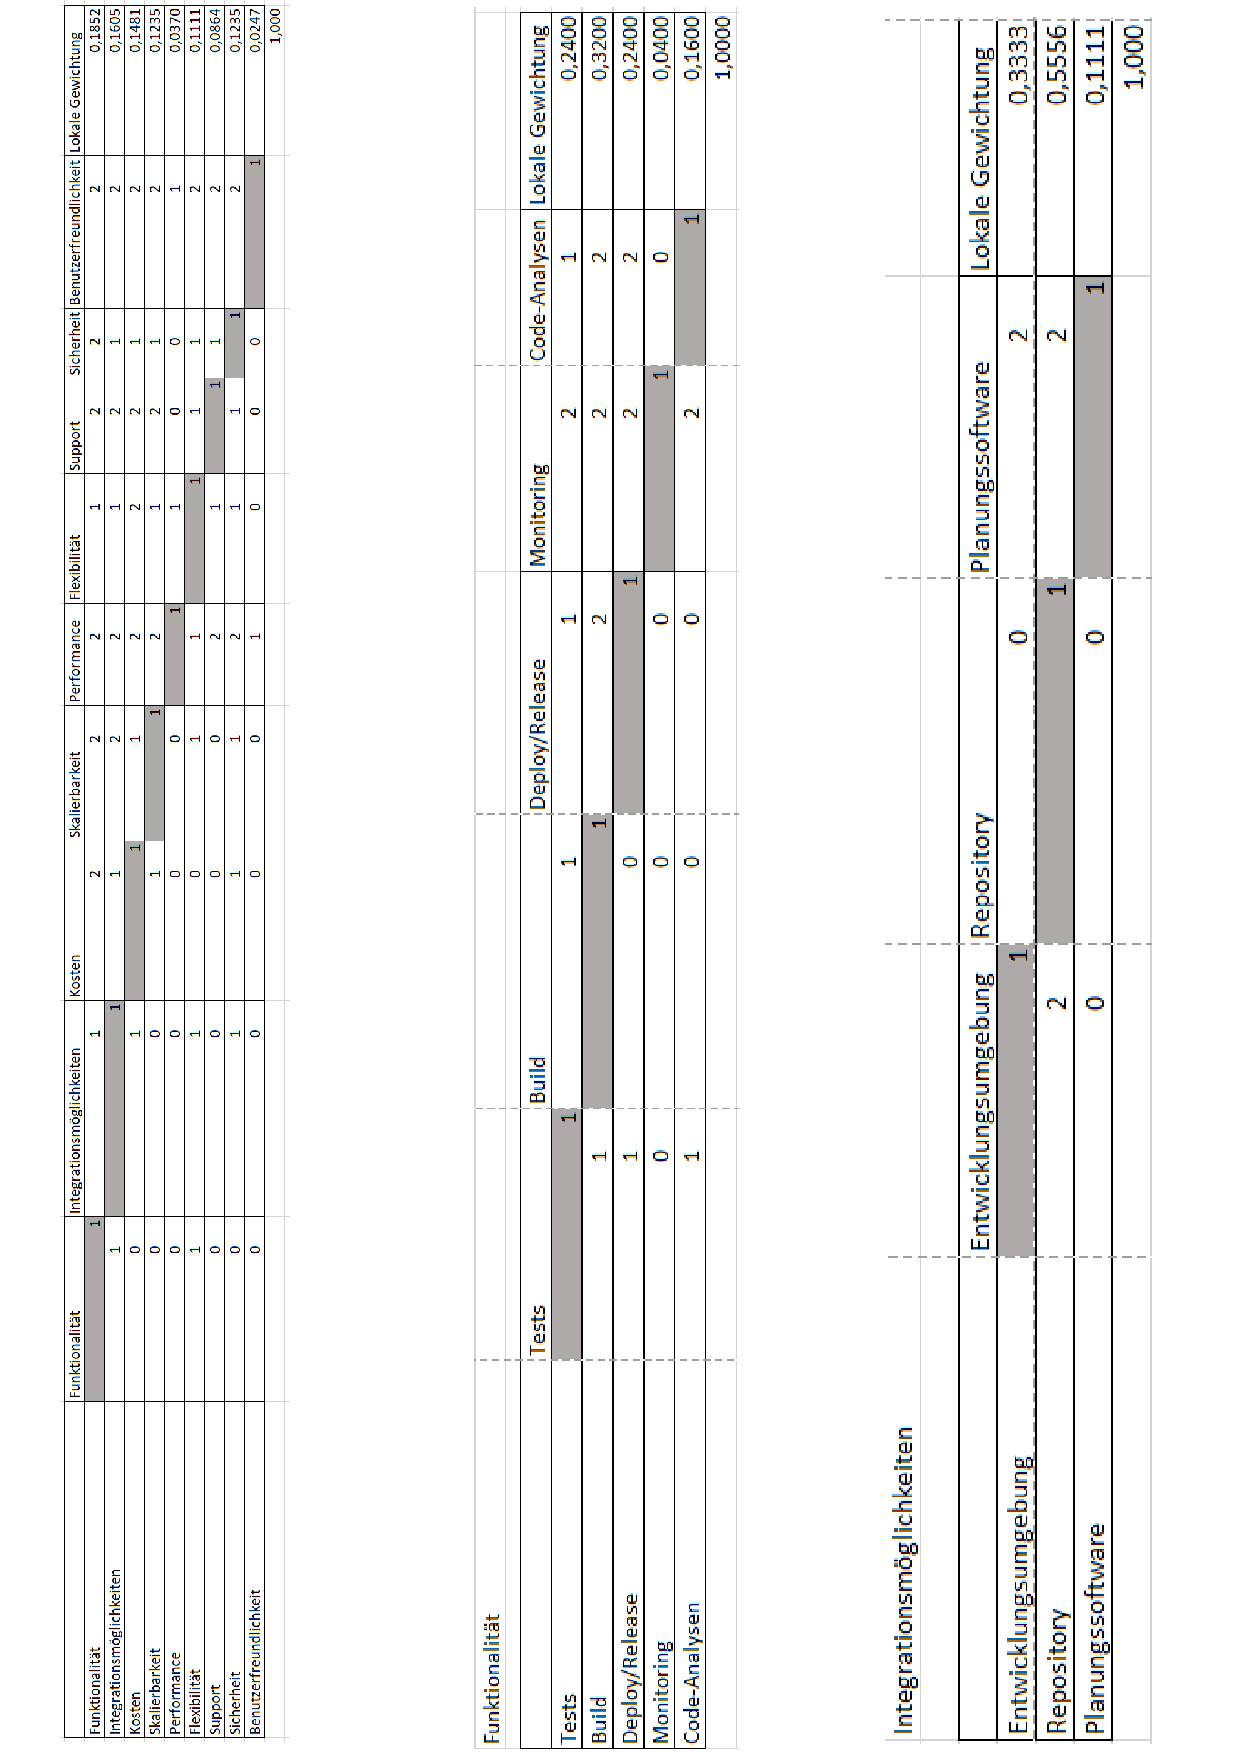
\includegraphics{Soelker_1}}
            \label{fig:gew_11}
        \end{figure}	
    \end{center}
    \begin{center}
        \begin{figure}[H]
            \centering
            \scalebox{0.7}{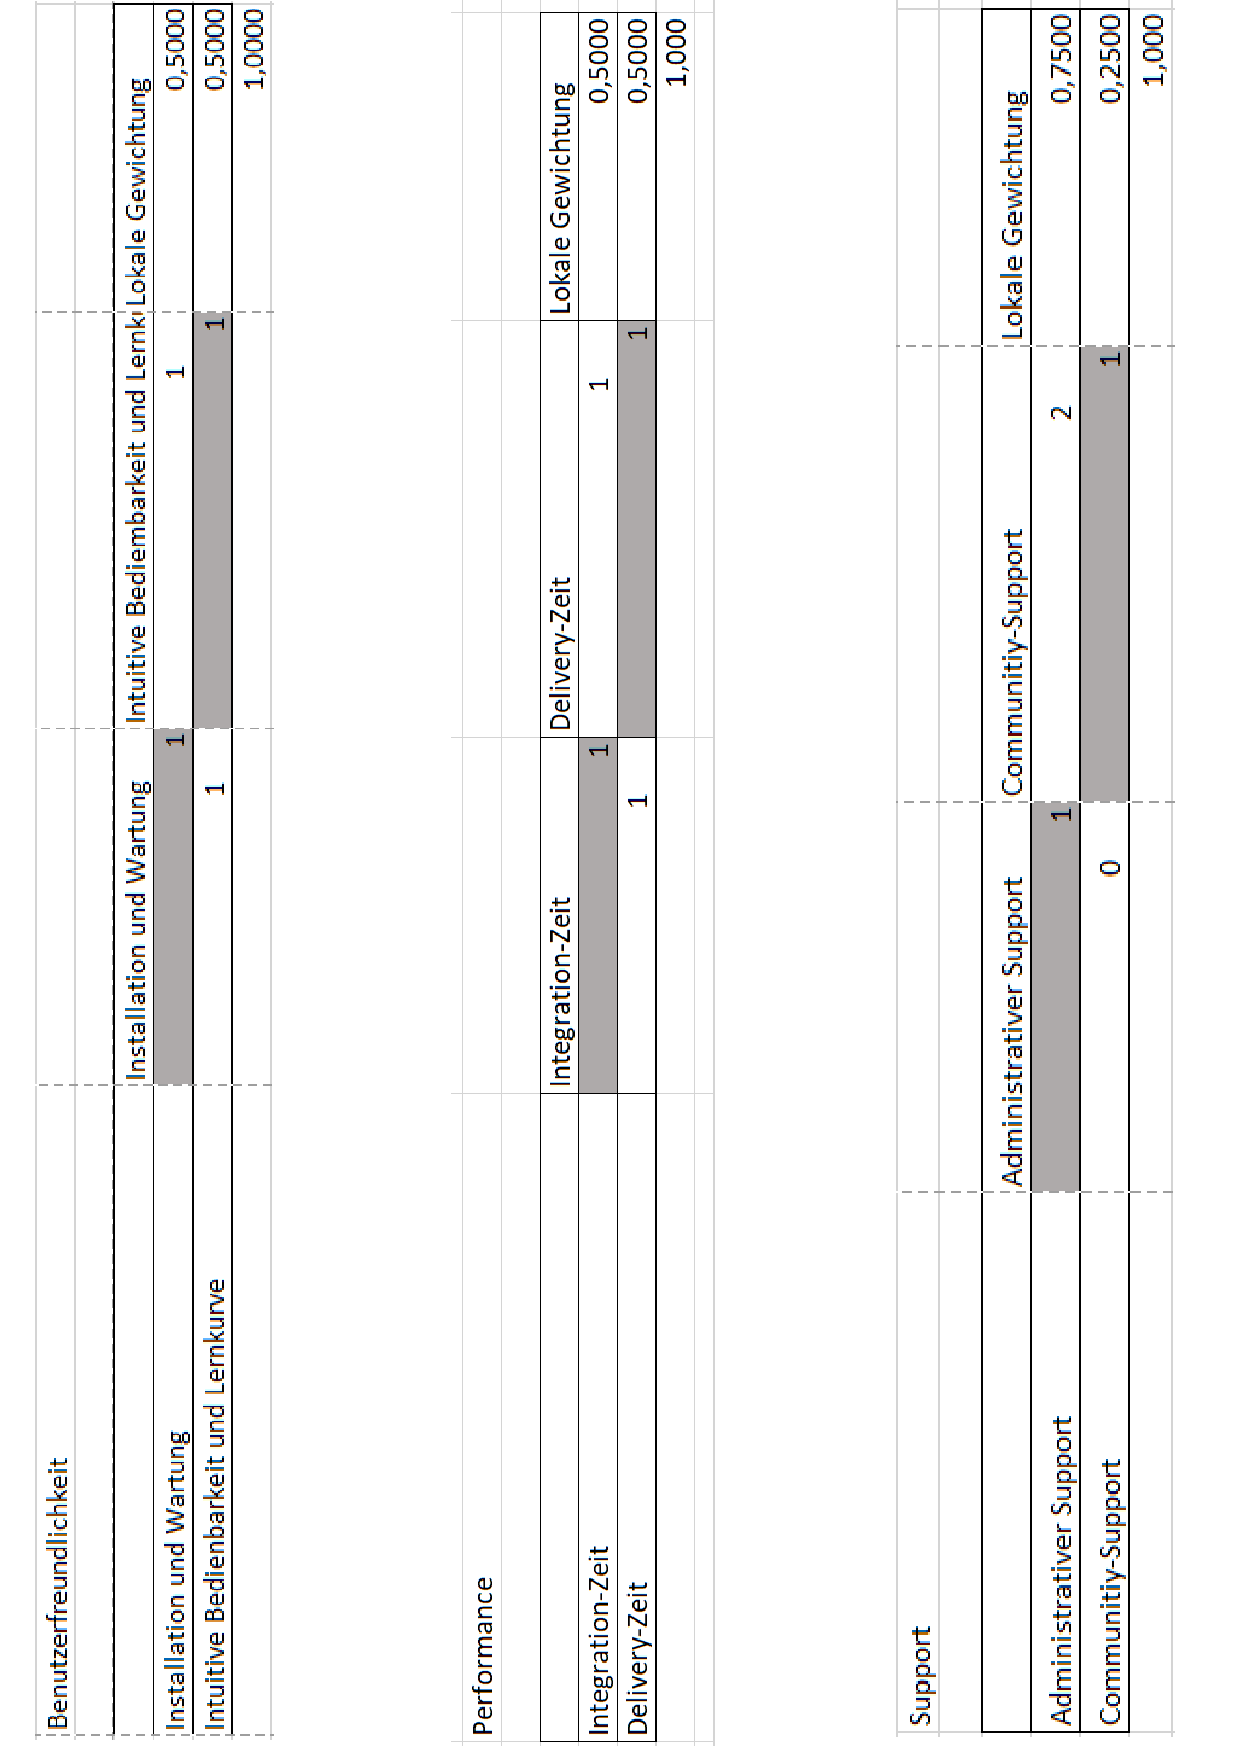
\includegraphics{Soelker_2}}
            \label{fig:gew_12}
        \end{figure}	
    \end{center}

    \begin{center}
        \begin{figure}[H]
            \centering
            \scalebox{0.7}{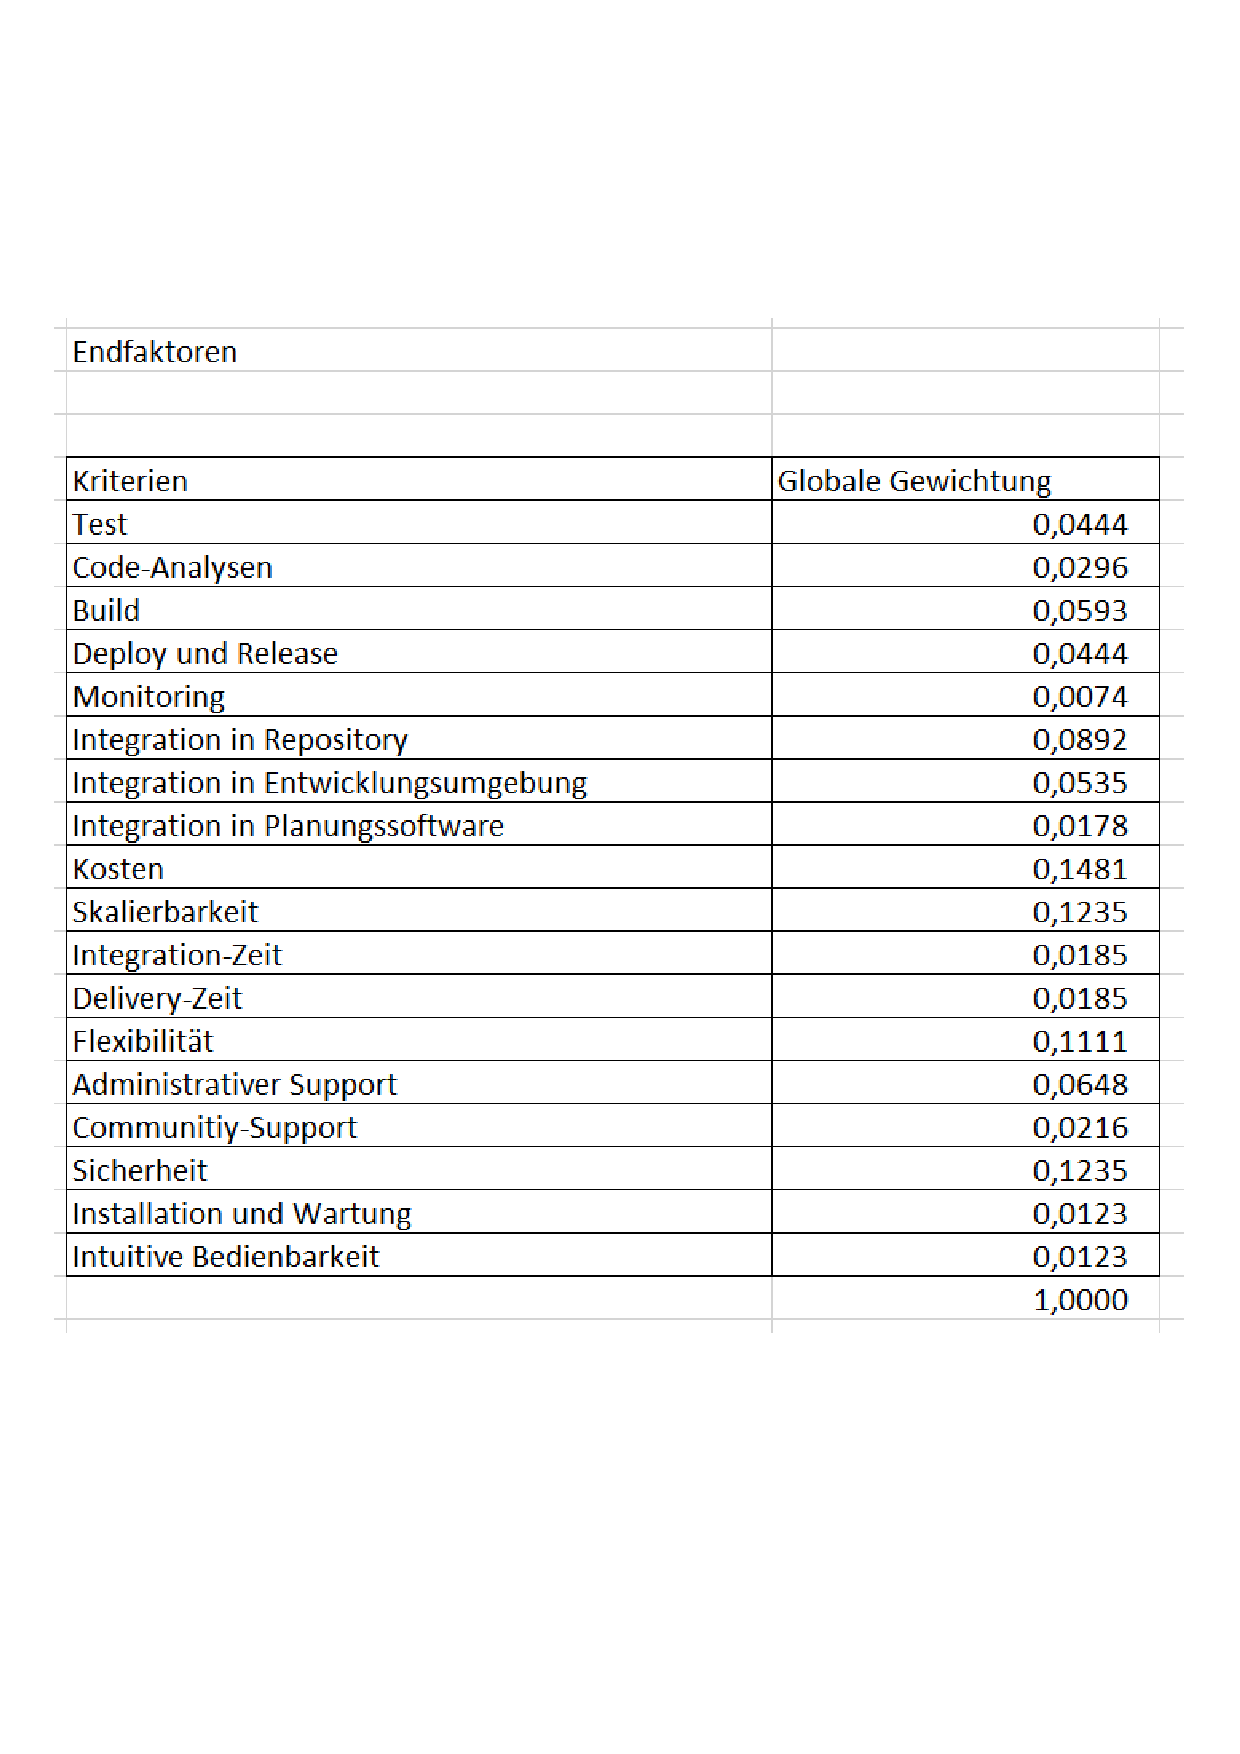
\includegraphics{Soelker_3}}
            \label{fig:gew_13}
        \end{figure}	
    \end{center}
    \newpage
    \resetlinenumber
    \begin{linenumbers}
        \textbf{Interviewer:} Für dich besonders wichtig ist die Funktionalität. Kannst du das begründen?\\
        \textbf{Experte:} Wenn ich eine Pipeline einbaue, dann ist für mich besonders wichtig, dass die Pipelines bestimmte Funktionalitäten, wie z.B. Tests abdecken. Weniger gewichtig ist da z.B. die Benutzerfreundlichkeit. Ich bin der Meinung, dass ich eine Pipeline einmalig einrichte. Da spielt es dann auch weniger die Rolle, wie viel Aufwand das beim initialen Einrichten erfordert hat. Beim Implementieren der Pipelines sieht das meiner Meinung nach ein wenig anders aus. So sollte ein Unternehmen zunächst damit beginnen; einfache Prozesse in der CI/CD-Pipeline zu automatisieren. Dann kann schrittweise immer mehr in die Pipeline eingebunden werden.\\
            \textbf{Interviewer:} Von den Subkriterien der Funktionalität war für dich die Build-Funktionalität besonders essenziell. Kannst du das begründen?\\
            \textbf{Experte:} Bei Cloud-Native-Projekten werden i.d.R. verschiedene Sprachen und verschiedene Frameworks verwendet. Die Pipeline sollte da einfach alle Build-Packages unterstützen. So muss ich dann nicht hergehen und manuell irgendwelche Deployments ausführen. Tests waren für mich auch sehr wichtig. Es ist wichtig, dass die Tests ausgeführt werden, bevor Code in dem Main-Branch zusammengeführt wird. Natürlich kann ich auch Tests abseits von einer CI/CD-Pipeline ausführen. Bei einem größeren Team von Entwickler ist das jedoch kaum noch kontrollierbar.\\
            \textbf{Interviewer:} Kommen wir zu den Integrationsmöglichkeiten. Deiner Meinung nach ist die Integration eines Repositorys sehr wichtig. Woran liegt das?\\
            \textbf{Experte:} Oft ist es so, dass sich der Kunde auf eine oder zwei CI/CD-Tools und ein oder zwei Repositorys einschießt. Gerade, wenn, da die Abhängigkeit mit dem Repository besteht, sollte das natürlich in die CI/CD-Pipeline integrierbar sein.\\
            \textbf{Interviewer:} Kannst du begründen, warum für dich die Integration- und Delivery-Zeit gleich wichtig sind.\\
            \textbf{Experte:} Aus meiner Sicht gibt es da kein wichtigeres Kriterium, da sowohl CI als auch CD im Hintergrund läuft. Somit ist es für mich jetzt nicht so wichtig, falls eine der beiden Pipelines länger durchläuft.\\
            \textbf{Interviewer:} Warum ist für dich der administrative Support wichtiger als der Community-Support?\\
            \textbf{Experte:} Für mich ist es eben sehr wichtig, dass es eine gute Dokumentation gibt. So kann ich z.B., bevor ich eine Pipeline installiere, schon abschätzen, wie gut bestimmte Aspekte funktioniere und ich bin nicht davon abhängig, dass ich durch Community-Foren irgendwelche Workarounds bekomme. Außerdem ist es mir natürlich auch sehr wichtig, dass die Lösung immer auf dem neusten Stand der Technik ist.\\
            \textbf{Interviewer:} Kannst du noch einmal deine Entscheidung zur Sicherheit begründen?\\
            \textbf{Experte:} Also es gehört natürlich einfach zur Developer-Experience dazu, wenn man bestimmte Authentifizierungs- und Autorisierungskonzepte hat. Dann ist es natürlich aber auch schon wichtig, dass die Pipeline an sich sicher ist. Gerade die Pipeline bietet natürlich eine sehr gute Möglichkeit, feindliche Programme in eine Produktionsumgebung einzuführen.\\
    \end{linenumbers}
    

    
    \newpage
    \subsection{Expertengewichtung 2}
            \begin{tabular}{ l l }
        Interviewpartner: & Full-Stack-Entwickler SAP DTS Integration (Experte 6)\\
        Datum: & 21.03.2023\\
        Interview-Medium: & Microsoft-Teams\\
\end{tabular}
\begin{center}
    \begin{figure}[H]
        \centering
        \scalebox{0.6}{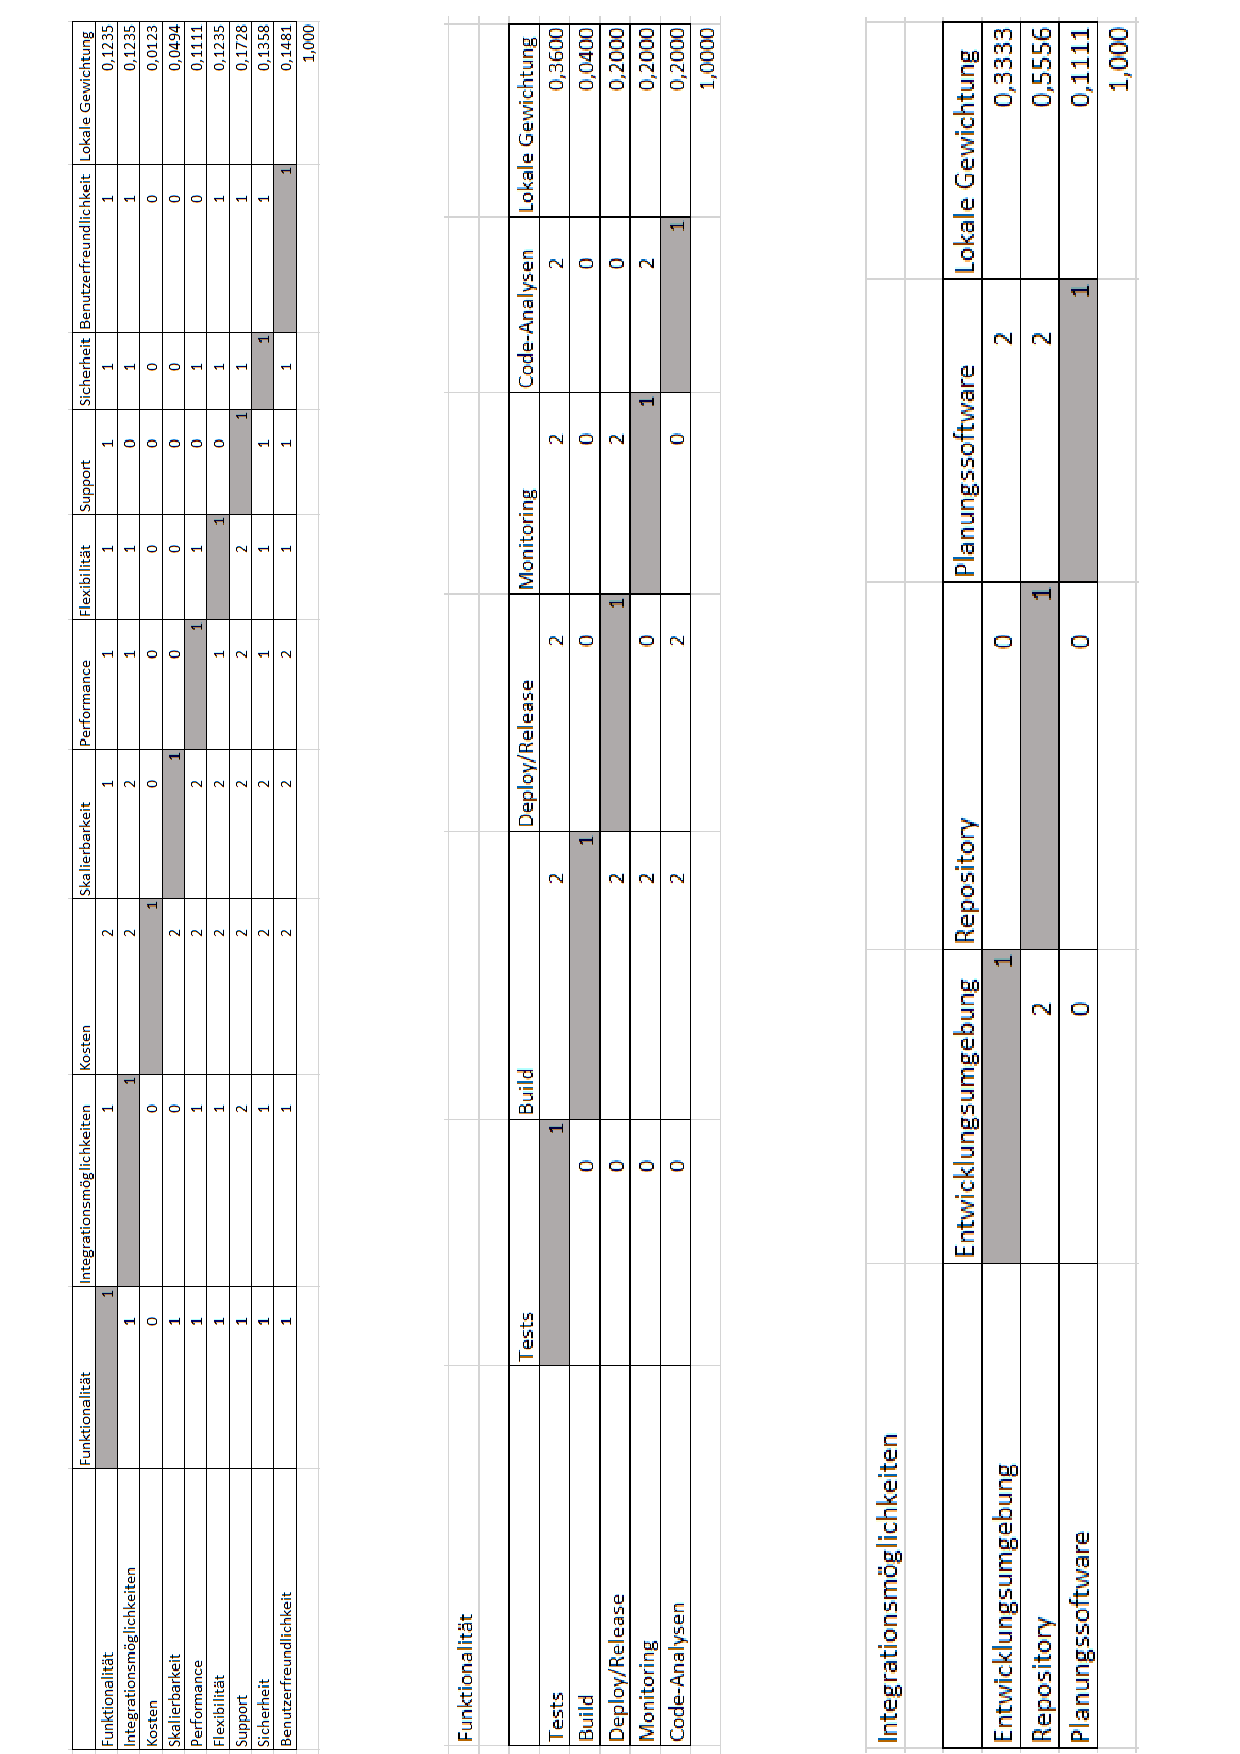
\includegraphics{Trump_1}}
        \label{fig:gew_21}
    \end{figure}	
\end{center}
\begin{center}
    \begin{figure}[H]
        \centering
        \scalebox{0.7}{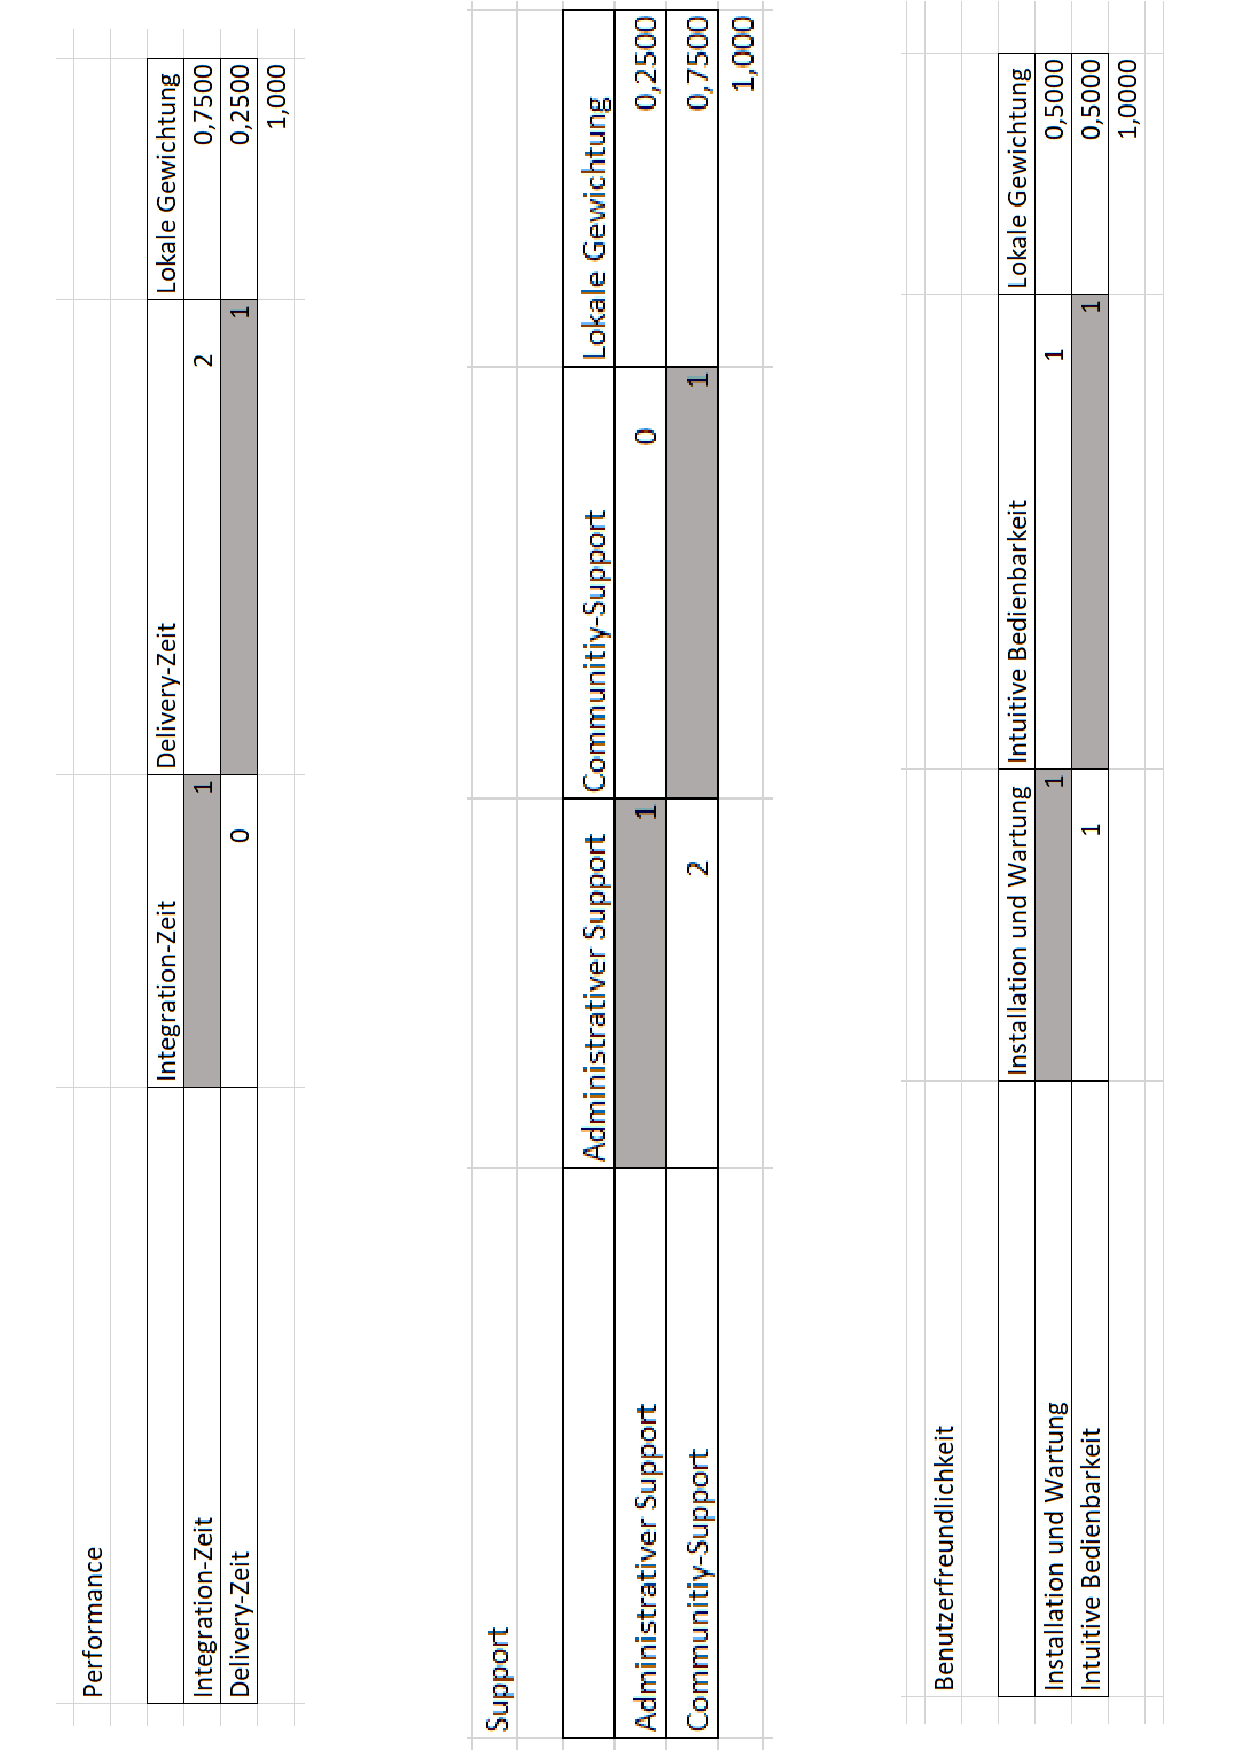
\includegraphics{Trump_2}}
        \label{fig:gew_22}
    \end{figure}	
\end{center}

\begin{center}
    \begin{figure}[H]
        \centering
        \scalebox{0.7}{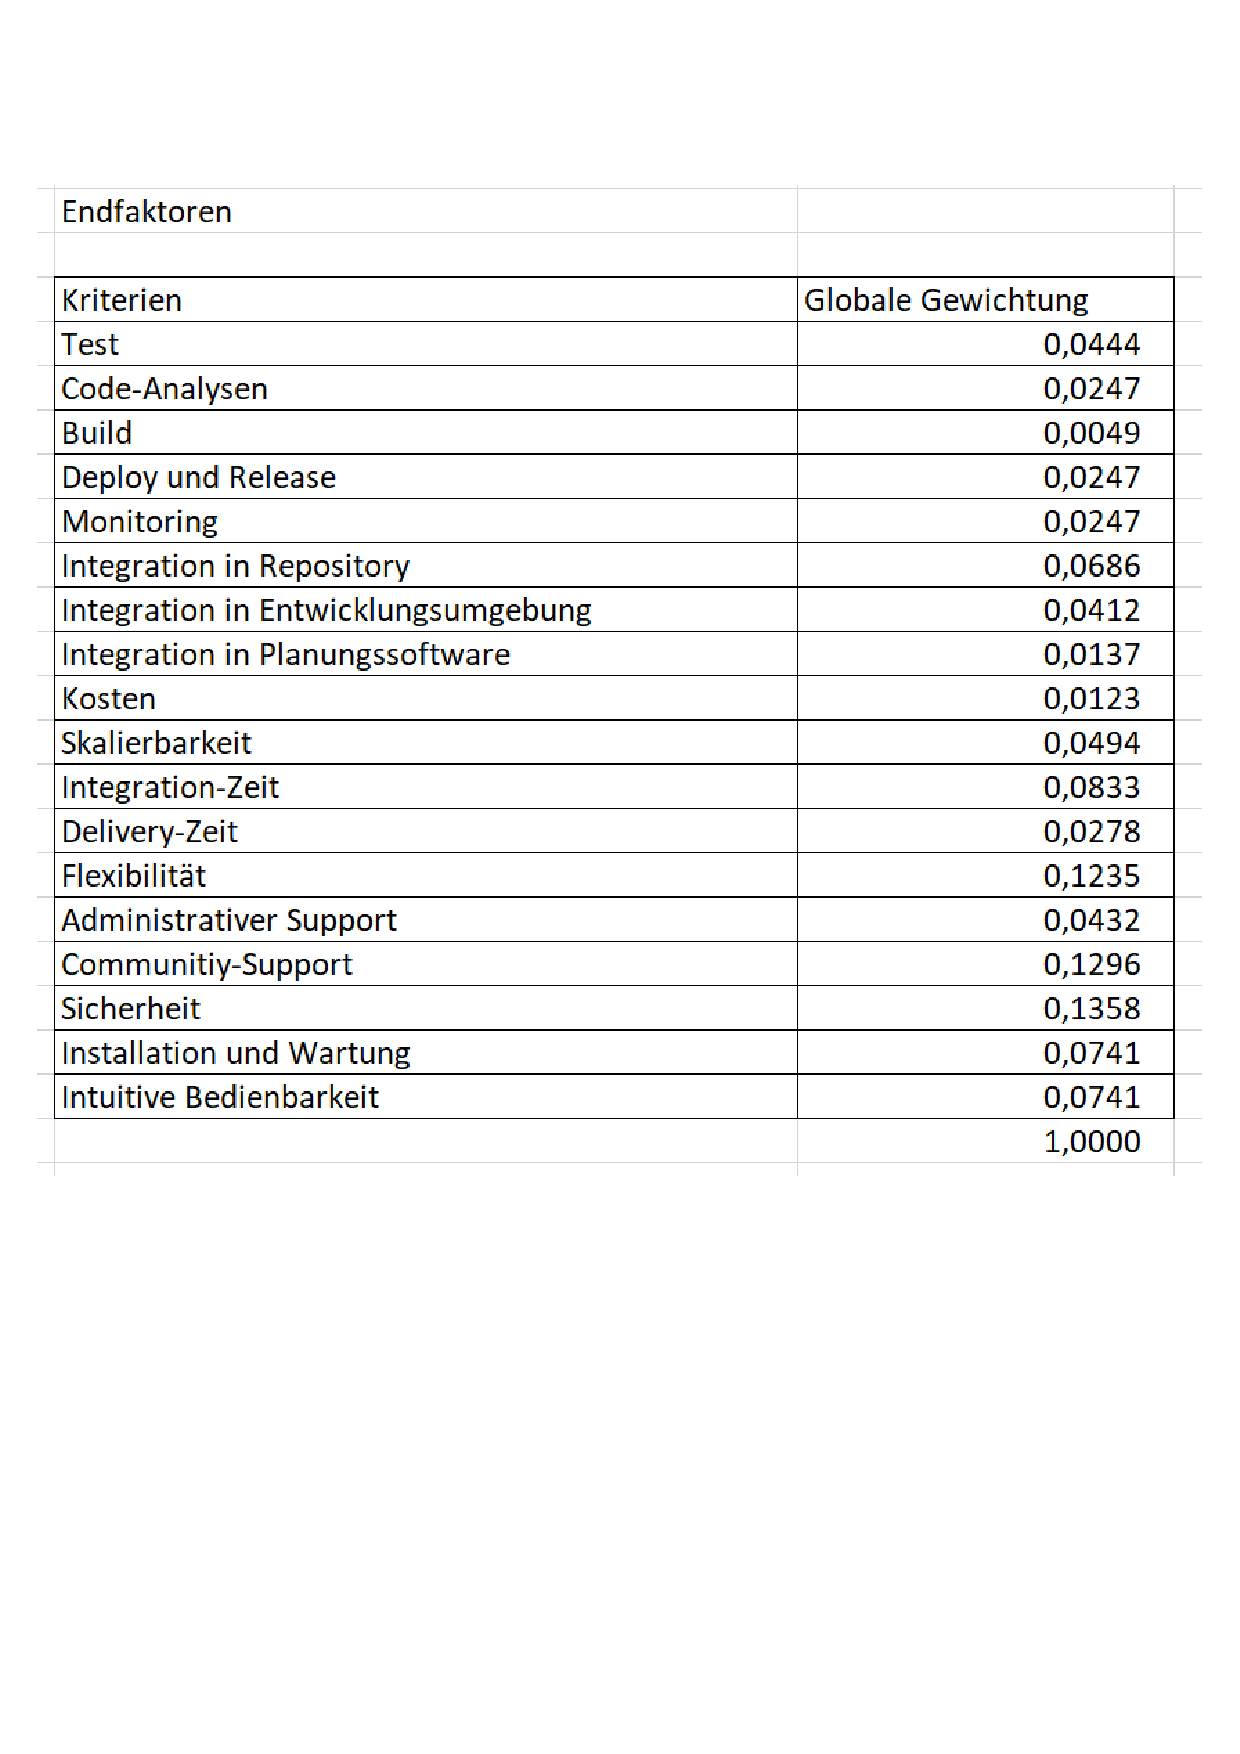
\includegraphics{Trump_3}}
        \label{fig:gew_23}
    \end{figure}	
\end{center}
\newpage

\resetlinenumber
\begin{linenumbers}
    \textbf{Interviewer}: In Tabelle 1 ist für dich besonders wichtig der Support und weniger wichtig sind für dich die Kosten. Warum?\\
    \textbf{Experte}: Ich als Entwickler habe die Erfahrung, dass ein Tool noch so toll sein kann. Wenn keine gute Dokumentation vorhanden ist, dann hilft mir das als Entwickler nicht viel. Die Kosten sind mir aus Entwicklersicht egal. Da sind mir erst mal die anderen Kriterien wichtiger.\\
    \textbf{Interviewer}: In Tabelle 2 waren dir die Tests besonders wichtig. Kannst du das begründen.\\
    \textbf{Experte:} Es spart mir sehr viel Zeit, wenn Tests automatisiert werden. Für mich gehört das automatisierte Ausführen von Tests auch zu den Hauptzwecken einer CI/CD-Pipeline. So kann ich frühzeitig erkennen, wenn eine Änderung etwas kaputt macht.\\
    \textbf{Interviewer:} Kommen wir zu den Integrationsmöglichkeiten. Warum ist dir die Integration in Repositorys besonders wichtig?\\
    \textbf{Experte:} Ich sehe, dass als eine sehr grundlegende Funktion. Wenn meine CI/CD-Pipeline nicht mit dem Repository integrierbar ist, dann wird das gesamte Konzept einer Pipeline hinfällig. Die Planungssoftware war mir hingegen nicht so wichtig, da ich als Entwickler mit so etwas kaum arbeite.\\
    \textbf{Interviewer:} Kannst du deine Entscheidungen zur Performance begründen?\\
    \textbf{Experte:} Für mich ist die Integration-Zeit deutlich wichtiger, einfach um eine bessere Developer-Experience zu bekommen. Wenn ich ein Pull-Request aufmache, dann möchte ich auch schnell Feedback bekommen. So kann ich dann evaluieren, ob alles passt oder eben nicht.\\
    \textbf{Interviewer:} Kannst du deine Entscheidungen zum Support begründen?\\
    \textbf{Experte:} Ich finde den Community-Support am wichtigsten. Dies ist als Entwickler die beste Möglichkeit, Zugriff auf neues Wissen zu erlangen. Weniger geeignet wäre, wenn ich jedes Mal mit jemandem telefonieren müsste oder immer ein neues Ticket aufmachen müsste. Weiterhin ist es sehr gut, wenn von einer Community Plug-ins bereitgestellt werden. Damit kann ich den Funktionsumfang erweitern. Jedoch besteht hier immer die Gefahr, dass Plug-ins Sicherheitslücken besitzen oder irgendwann nicht mehr richtig gewartet werden.\\
    \textbf{Interviewer:} Wie sieht es mit dem Punkt der Sicherheit aus?\\
    \textbf{Experte:} Ich finde das Authentifizierungs- und Autorisierungskonzept sehr wichtig, da dies mit der Developer-Experience zusammenhängt. Damit komme ich eben in meinem Entwickleralltag am meisten in Berührung. Wenn die Plattform bspw. SSO-enabled ist, dann ist das für mich als Programmierer sehr gemütlich.\\ 
    \textbf{Interviewer:} Kannst du deine Entscheidung zur Benutzerfreundlichkeit begründen?\\
    \textbf{Experte:} Sowohl mit Wartung bzw. Installation und mit der intuitiven Bedienbarkeit kommt man gelegentlich in Berührung. Das sollte deshalb beides einigermaßen gut funktionieren.\\
\end{linenumbers}

\newpage
\subsection{Expertengewichtung 3}
        \begin{tabular}{ l l }
    Interviewpartner: & Frontend-Test-Entwickler SAP Hyperspace (Experte 4)\\
    Datum: & 22.03.2023\\
    Interview-Medium: & Microsoft-Teams\\
\end{tabular}
\begin{center}
\begin{figure}[H]
    \centering
    \scalebox{0.6}{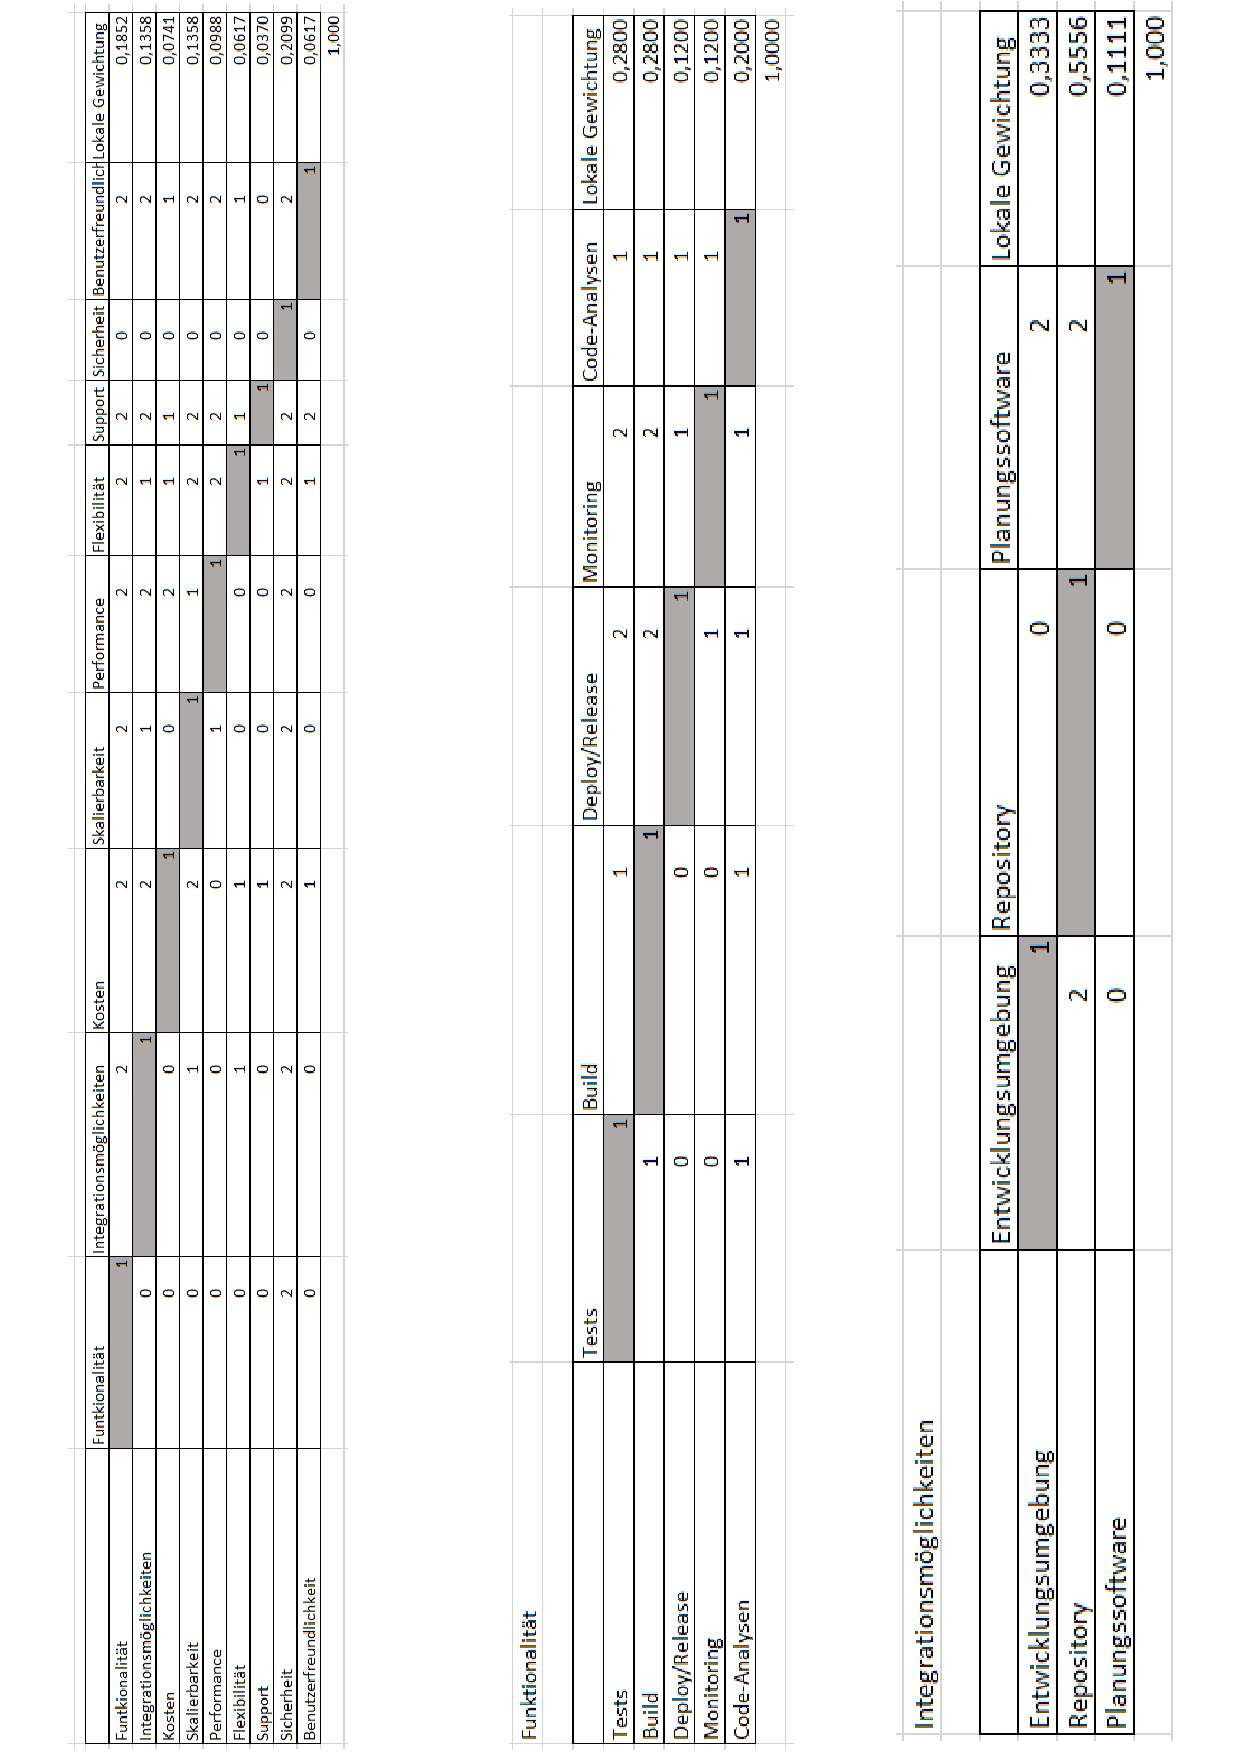
\includegraphics{Bischoff_1}}
    \label{fig:gew_31}
\end{figure}	
\end{center}
\begin{center}
\begin{figure}[H]
    \centering
    \scalebox{0.7}{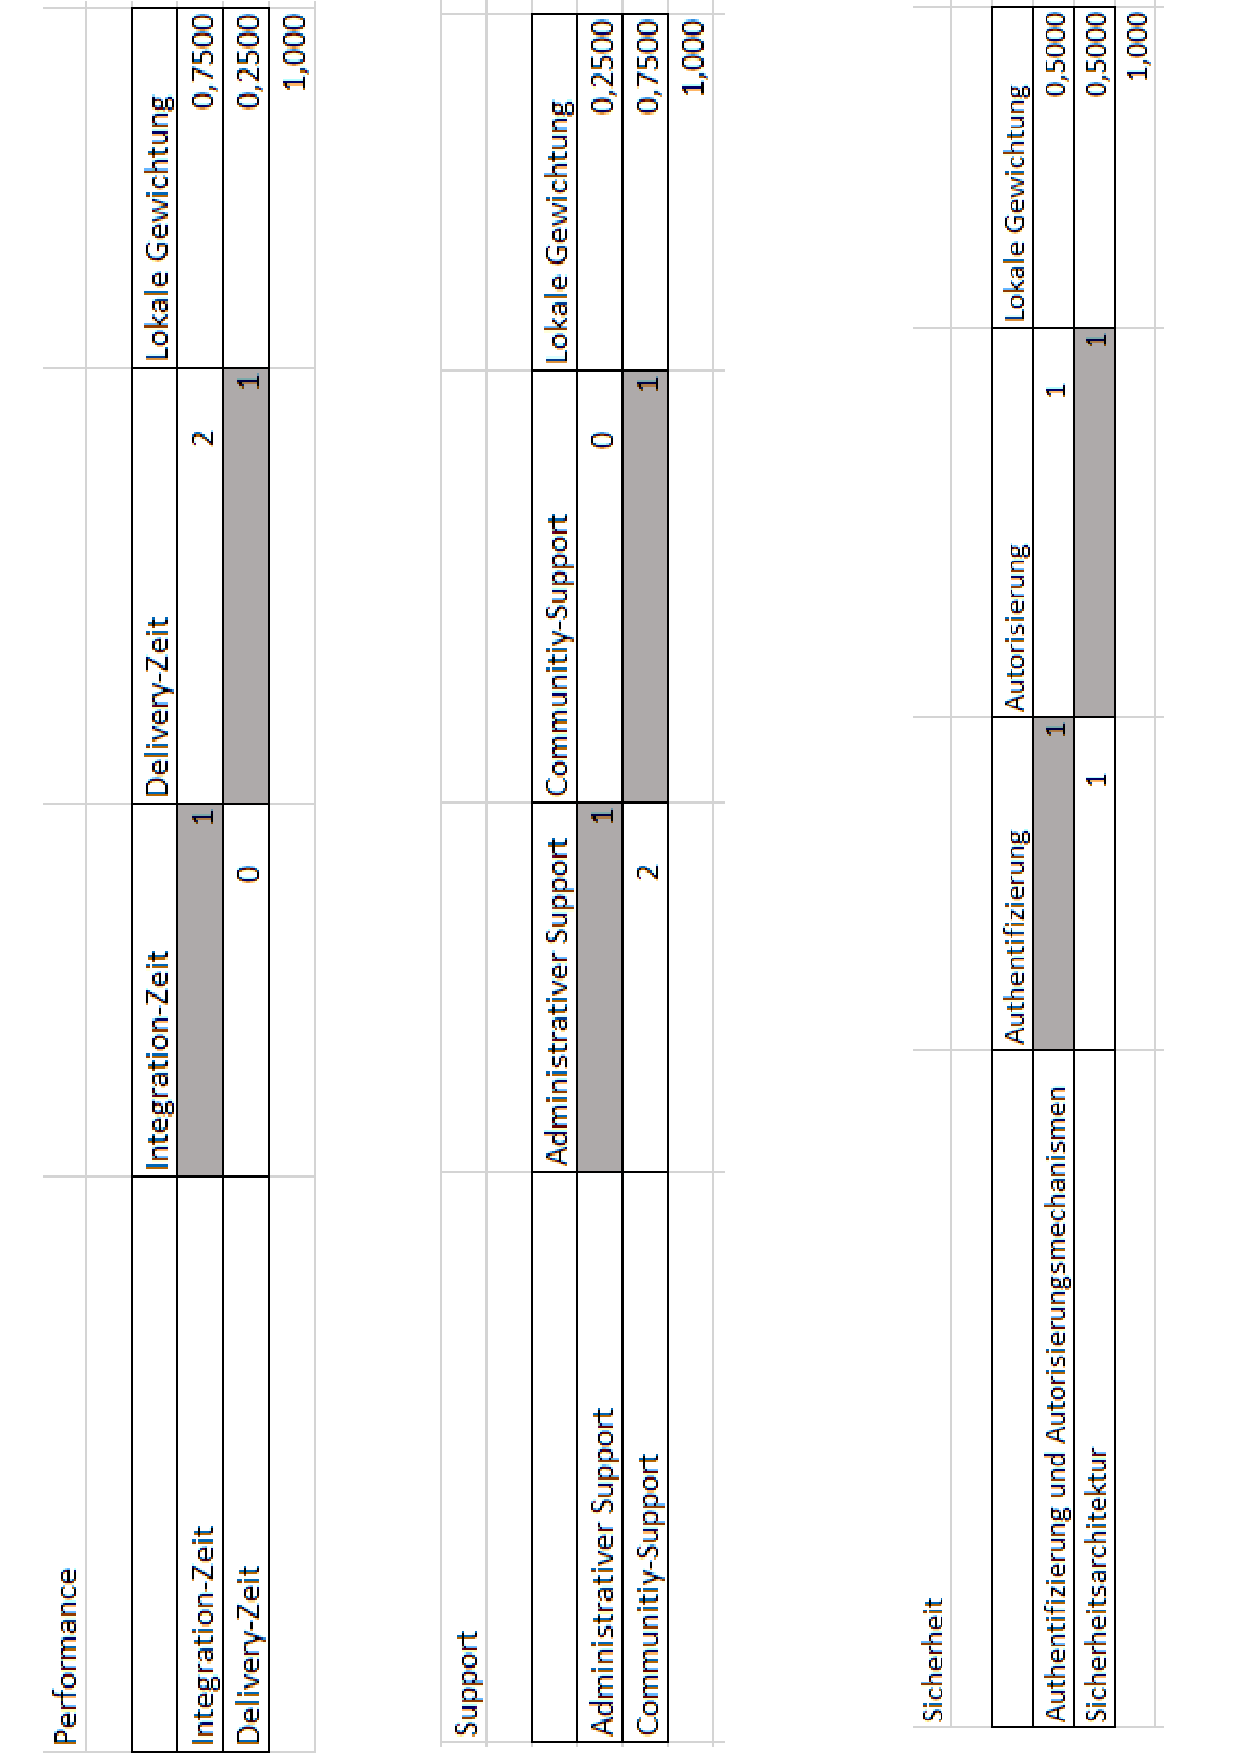
\includegraphics{Bischoff_2}}
    \label{fig:gew_32}
\end{figure}	
\end{center}

\begin{center}
\begin{figure}[H]
    \centering
    \scalebox{0.7}{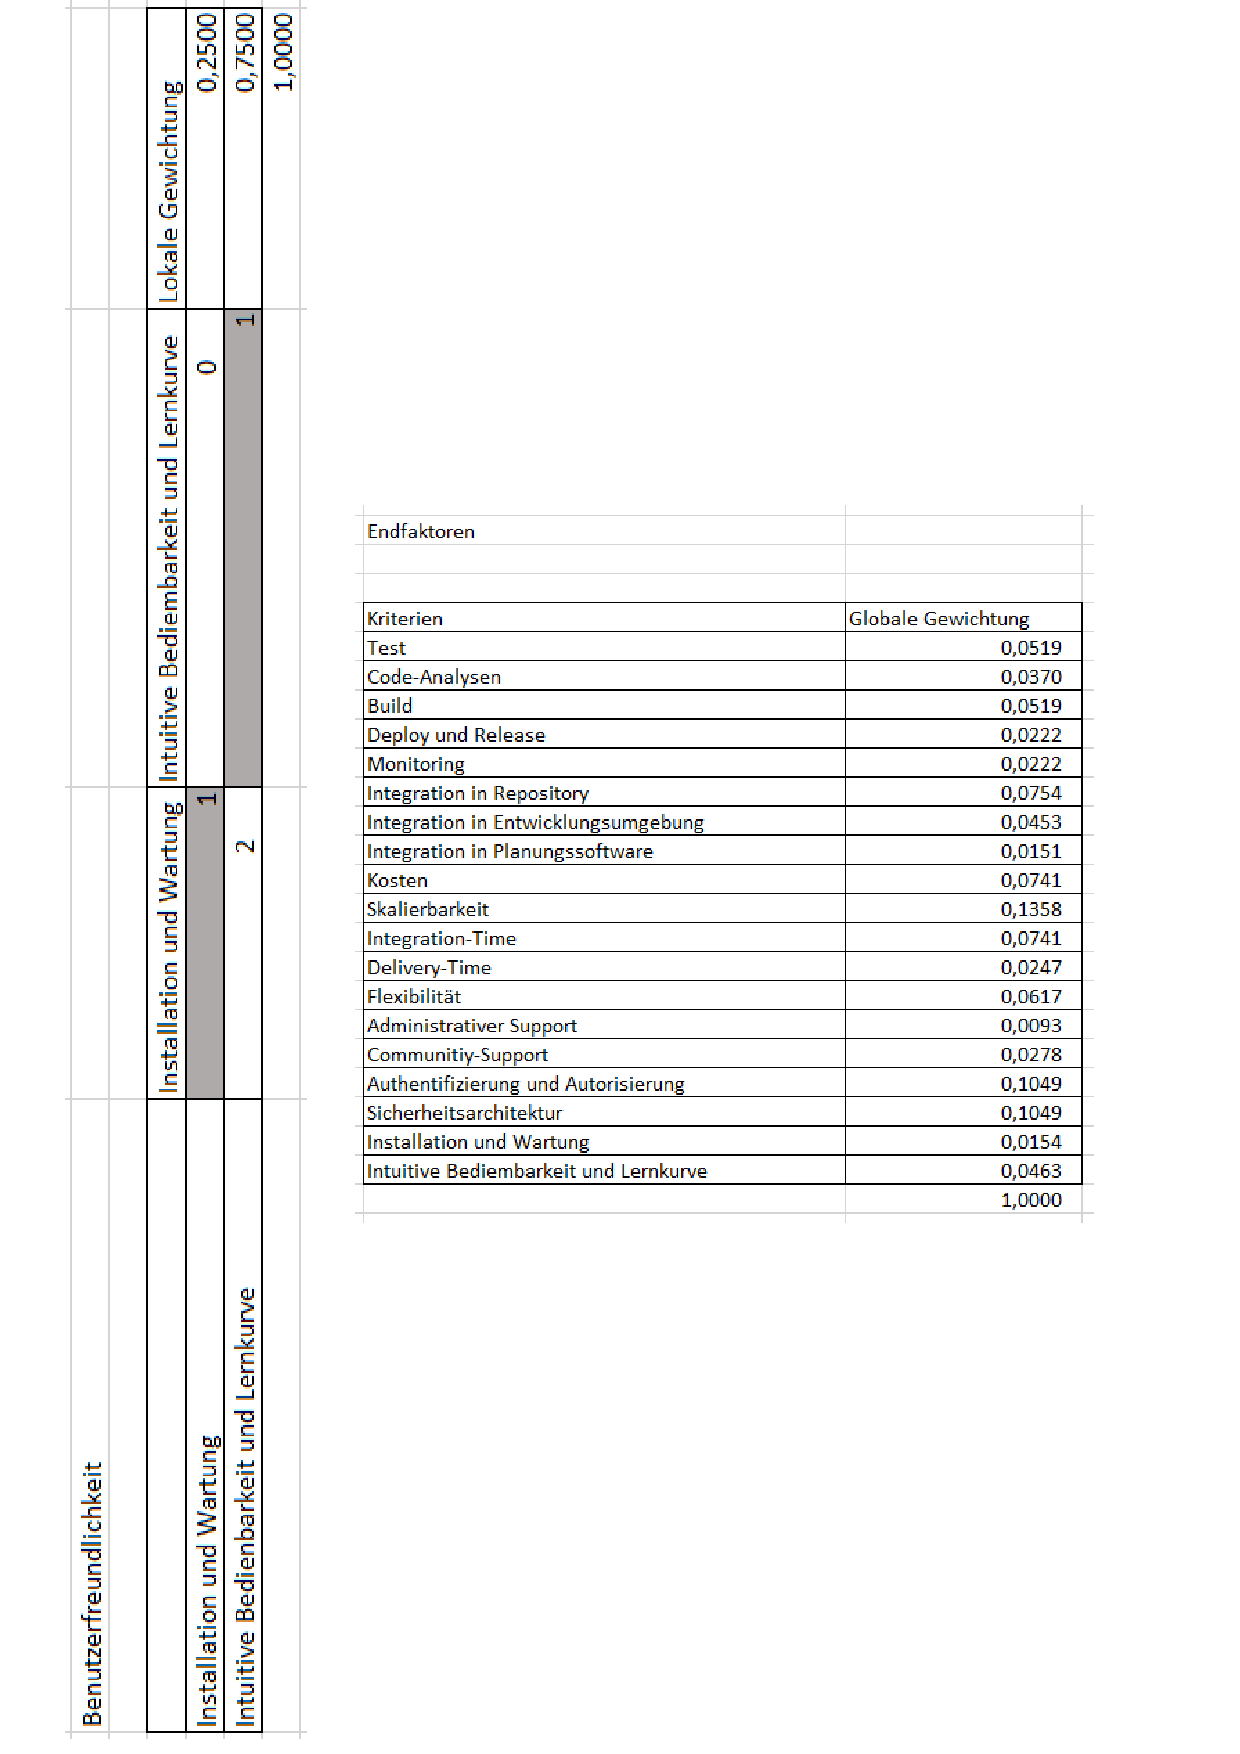
\includegraphics{Bischoff_3}}
    \label{fig:gew_33}
\end{figure}	
\end{center}
\newpage
\resetlinenumber
\begin{linenumbers}
    \textbf{Interviewer:} Besonders wichtig ist für dich die Sicherheit. Kannst du das begründen?\\
    \textbf{Experte:} Sicherheitslücken in unseren Systemen würden einen sehr großen Imageschaden verursachen. Deswegen ist das für mich das absolute Top-Thema. Gerade wenn wir neue Software bereitstellen, darf es nicht passieren, dass eventuell feindliche Programme eingeschleust werden. Nicht so wichtig ist für mich der Support, da ein Tool lieber eine hohe Benutzerfreundlichkeit besitzen sollte und wobei dann gar kein Support nötig wäre.\\
    \textbf{Interviewer:} Warum ist für dich der administrative Support wichtiger als der Community-Support?\\
    \textbf{Experte:} Es ist viel wichtiger, dass man eine Community besitzt, welche Fragen beantworten kann. Dies ist eigentlich die einzige Möglichkeit Support skalierbar zu machen. Man wird niemals ein Support-Team besitzen, was groß genug ist, alle Fragen zu beantworten. Man könnte den administrativen Support also nicht gut skalieren.\\
    \textbf{Interviewer:} Im Kriterium der Funktionalität ist für dich die Test- und Build-Funktionalität besonders wichtig. Warum?\\
    \textbf{Experte:} Test ist natürlich mein Hintergrund, da ich mich während meiner operativen Arbeit sehr viel damit beschäftige. Es ist für mich einfach wichtig, dass ich etwas ausliefere, was auch validiert ist.\\
    \textbf{Interviewer:} Warum ist für dich die Integration-Zeit wichtiger als die Delivery-Zeit?\\
    \textbf{Experte:} Es kann eben aus Entwicklersicht nicht sein, dass ich eine Änderung im Code mache und dann erst einmal eine halbe Stunde warten muss, bis ich Feedback bekomme. Da geht die Motivation im Team verloren. Und es stapeln sich einfach die Änderungen, bevor ich den Code dann tatsächlich ausliefere.\\
    \textbf{Interviewer:} Kannst du noch einmal deine Entscheidung zur Sicherheit begründen?\\
    \textbf{Experte:} Authentifizierung ist natürlich wichtig, damit jemand unberechtigtes eigenständig ein Deployment durchführen kann.\\
    \textbf{Interviewer:} Für dich war die Installation und Wartung weniger wichtig als die intuitive Bedienbarkeit?\\
    \textbf{Experte:} Installation und Wartung betrifft mich einmal beim Setup, während die intuitive Bedienbarkeit kontinuierlich wichtig anfällt, da mit dieser ja z.B. auch das Implementieren einer Pipeline gemeint ist.\\
\end{linenumbers}



\newpage
\subsection{Expertengewichtung 4}
        \begin{tabular}{ l l }
    Interviewpartner: & Backend-Test-Entwickler SAP DTS Integration (Experte 7)\\
    Datum: & 22.03.2023\\
    Interview-Medium: & Microsoft-Teams\\
\end{tabular}
\begin{center}
\begin{figure}[H]
    \centering
    \scalebox{0.6}{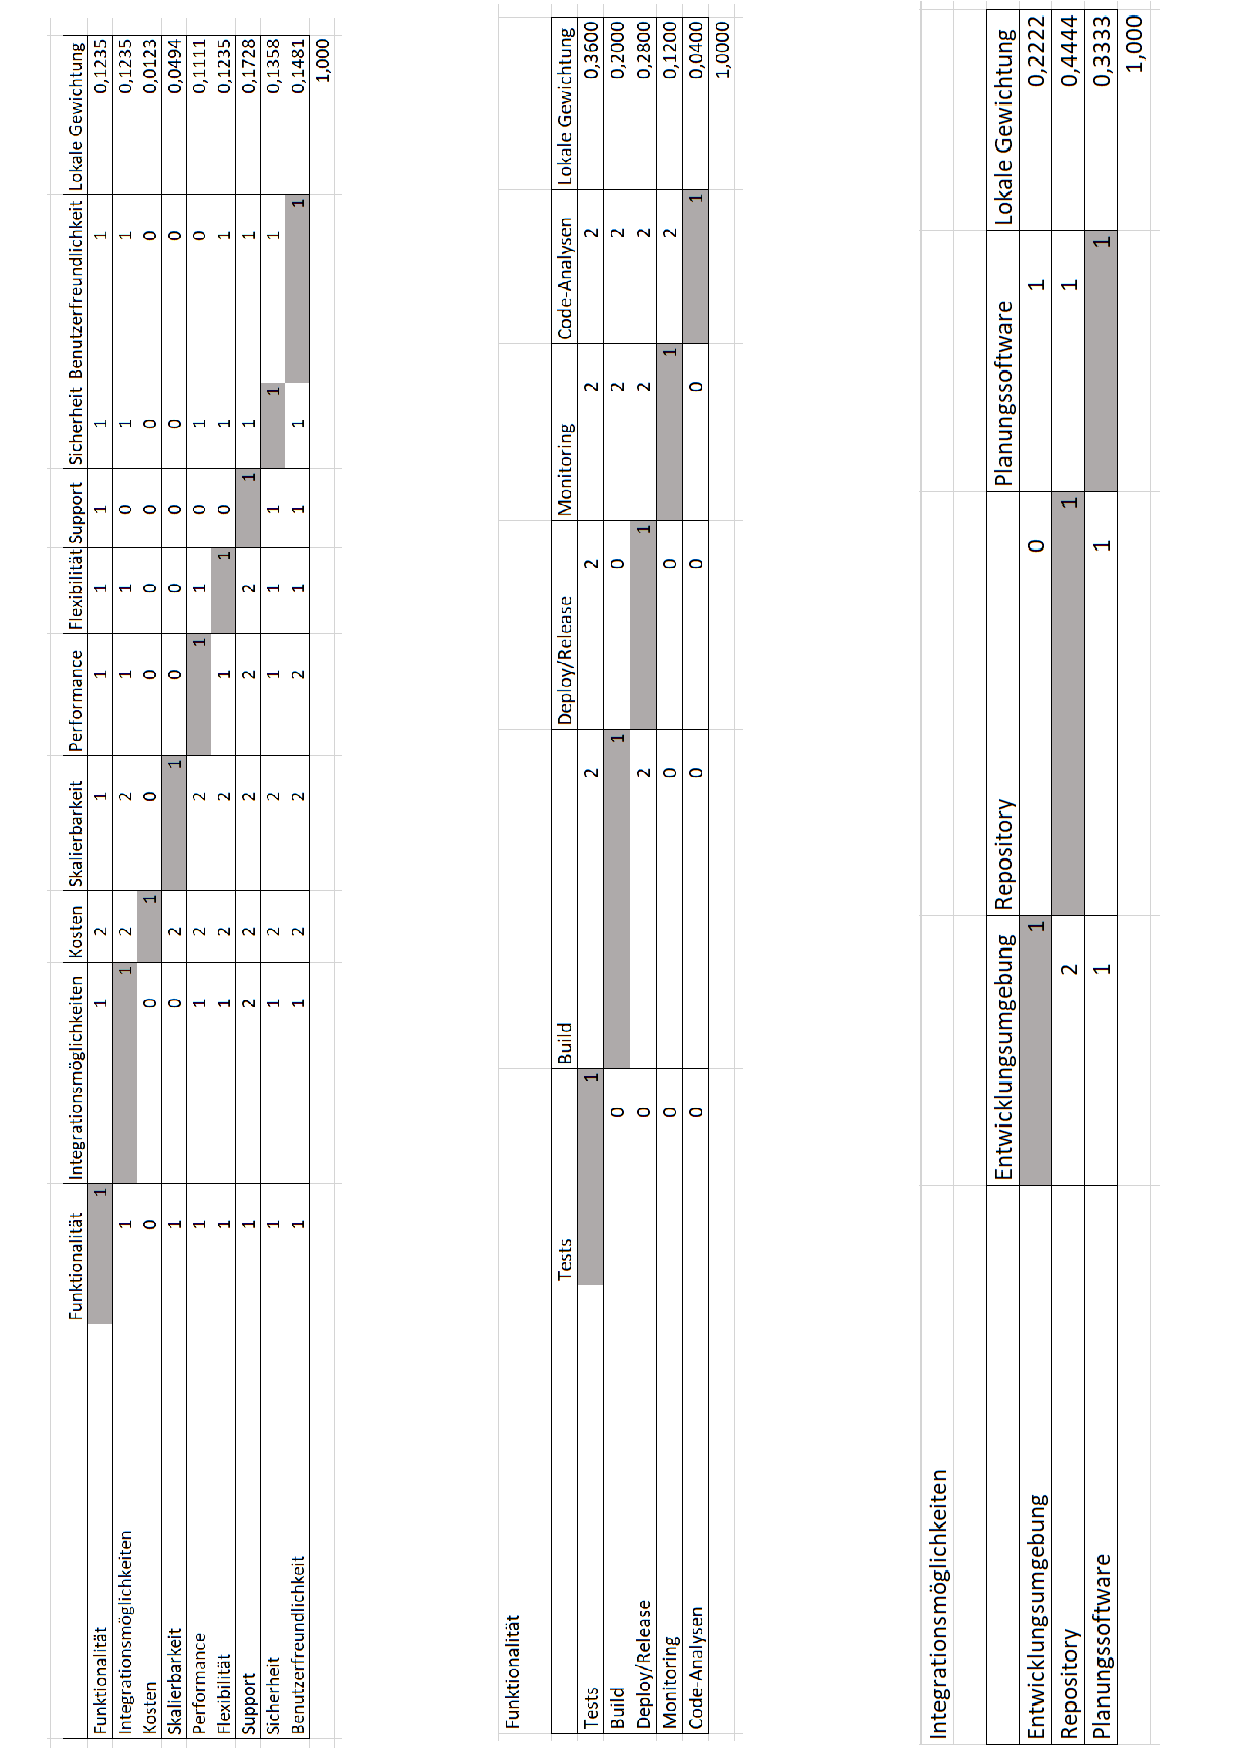
\includegraphics{Adams_1}}
    \label{fig:gew_41}
\end{figure}	
\end{center}
\begin{center}
\begin{figure}[H]
    \centering
    \scalebox{0.7}{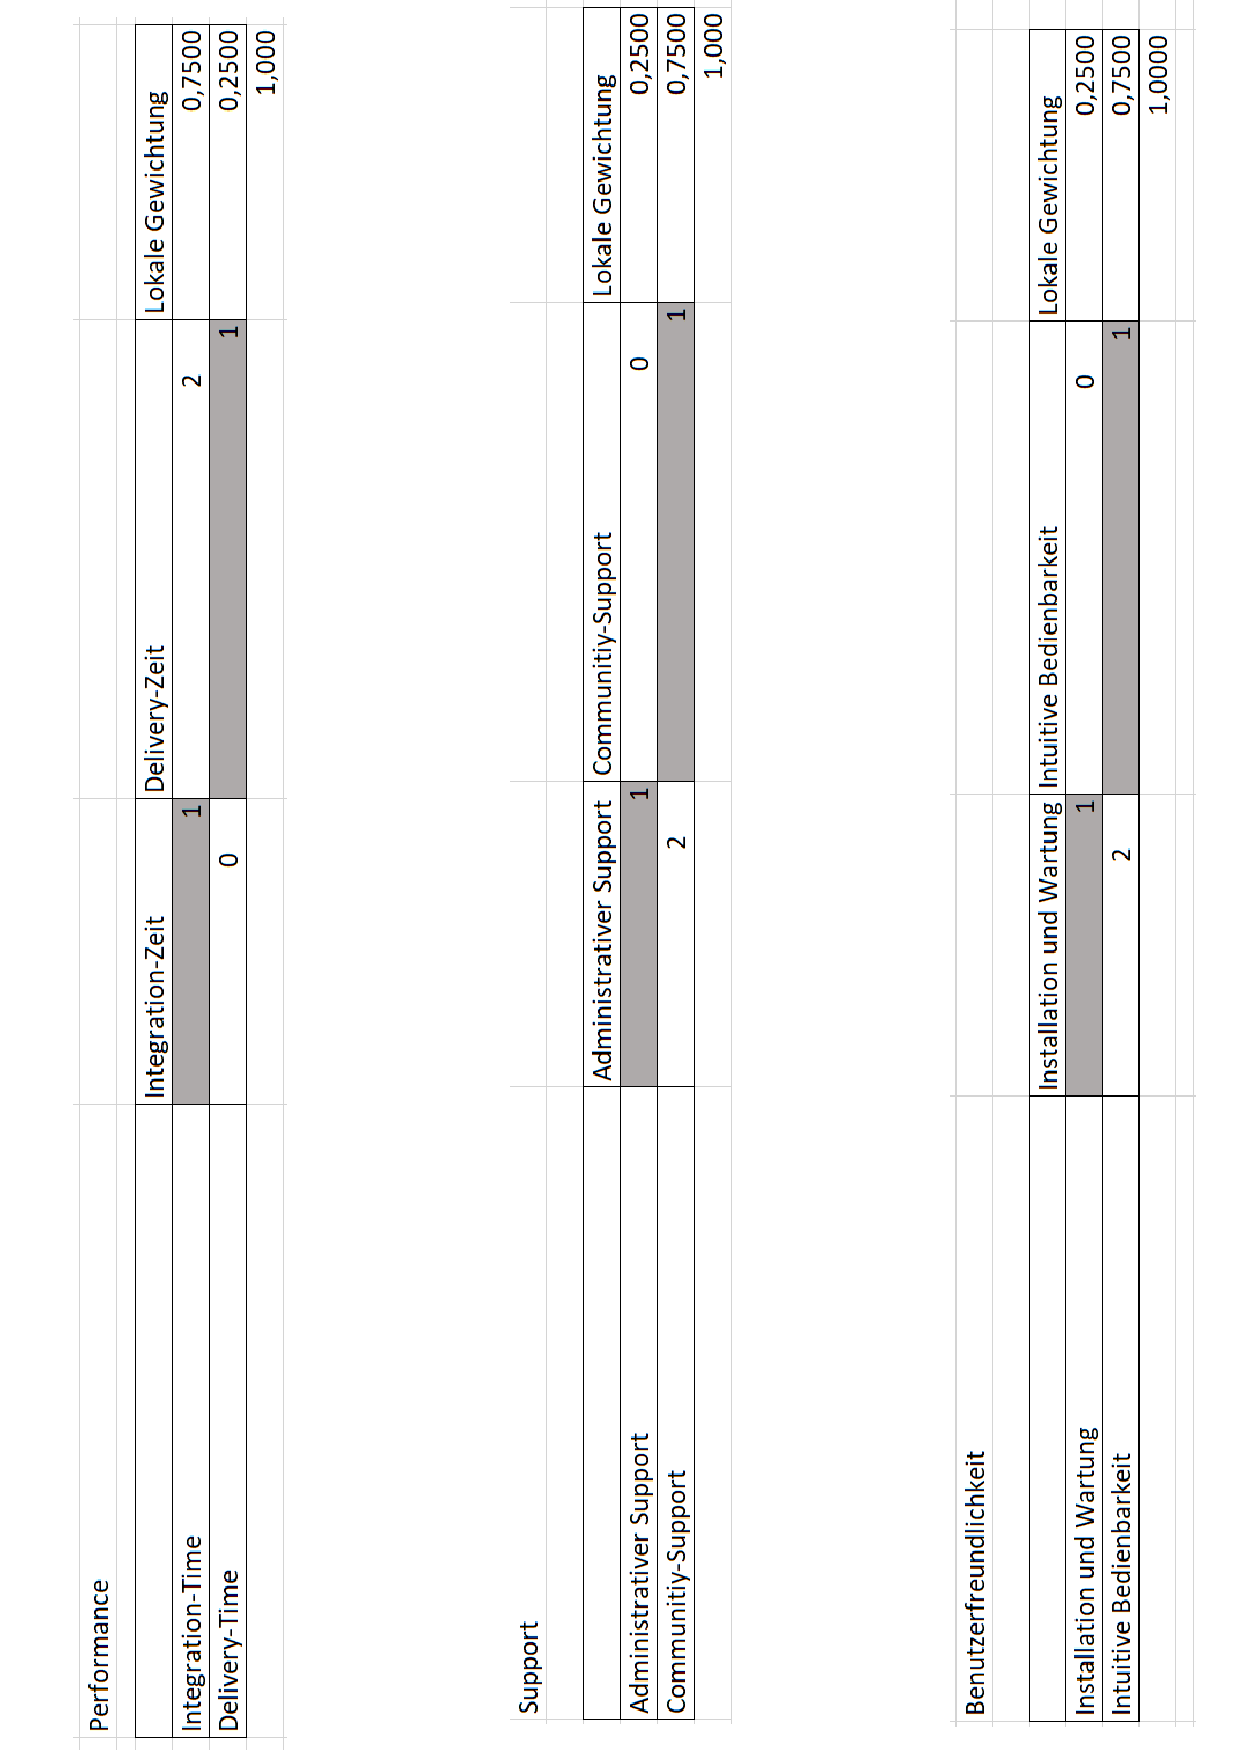
\includegraphics{Adams_2}}
    \label{fig:gew_42}
\end{figure}	
\end{center}

\begin{center}
\begin{figure}[H]
    \centering
    \scalebox{0.7}{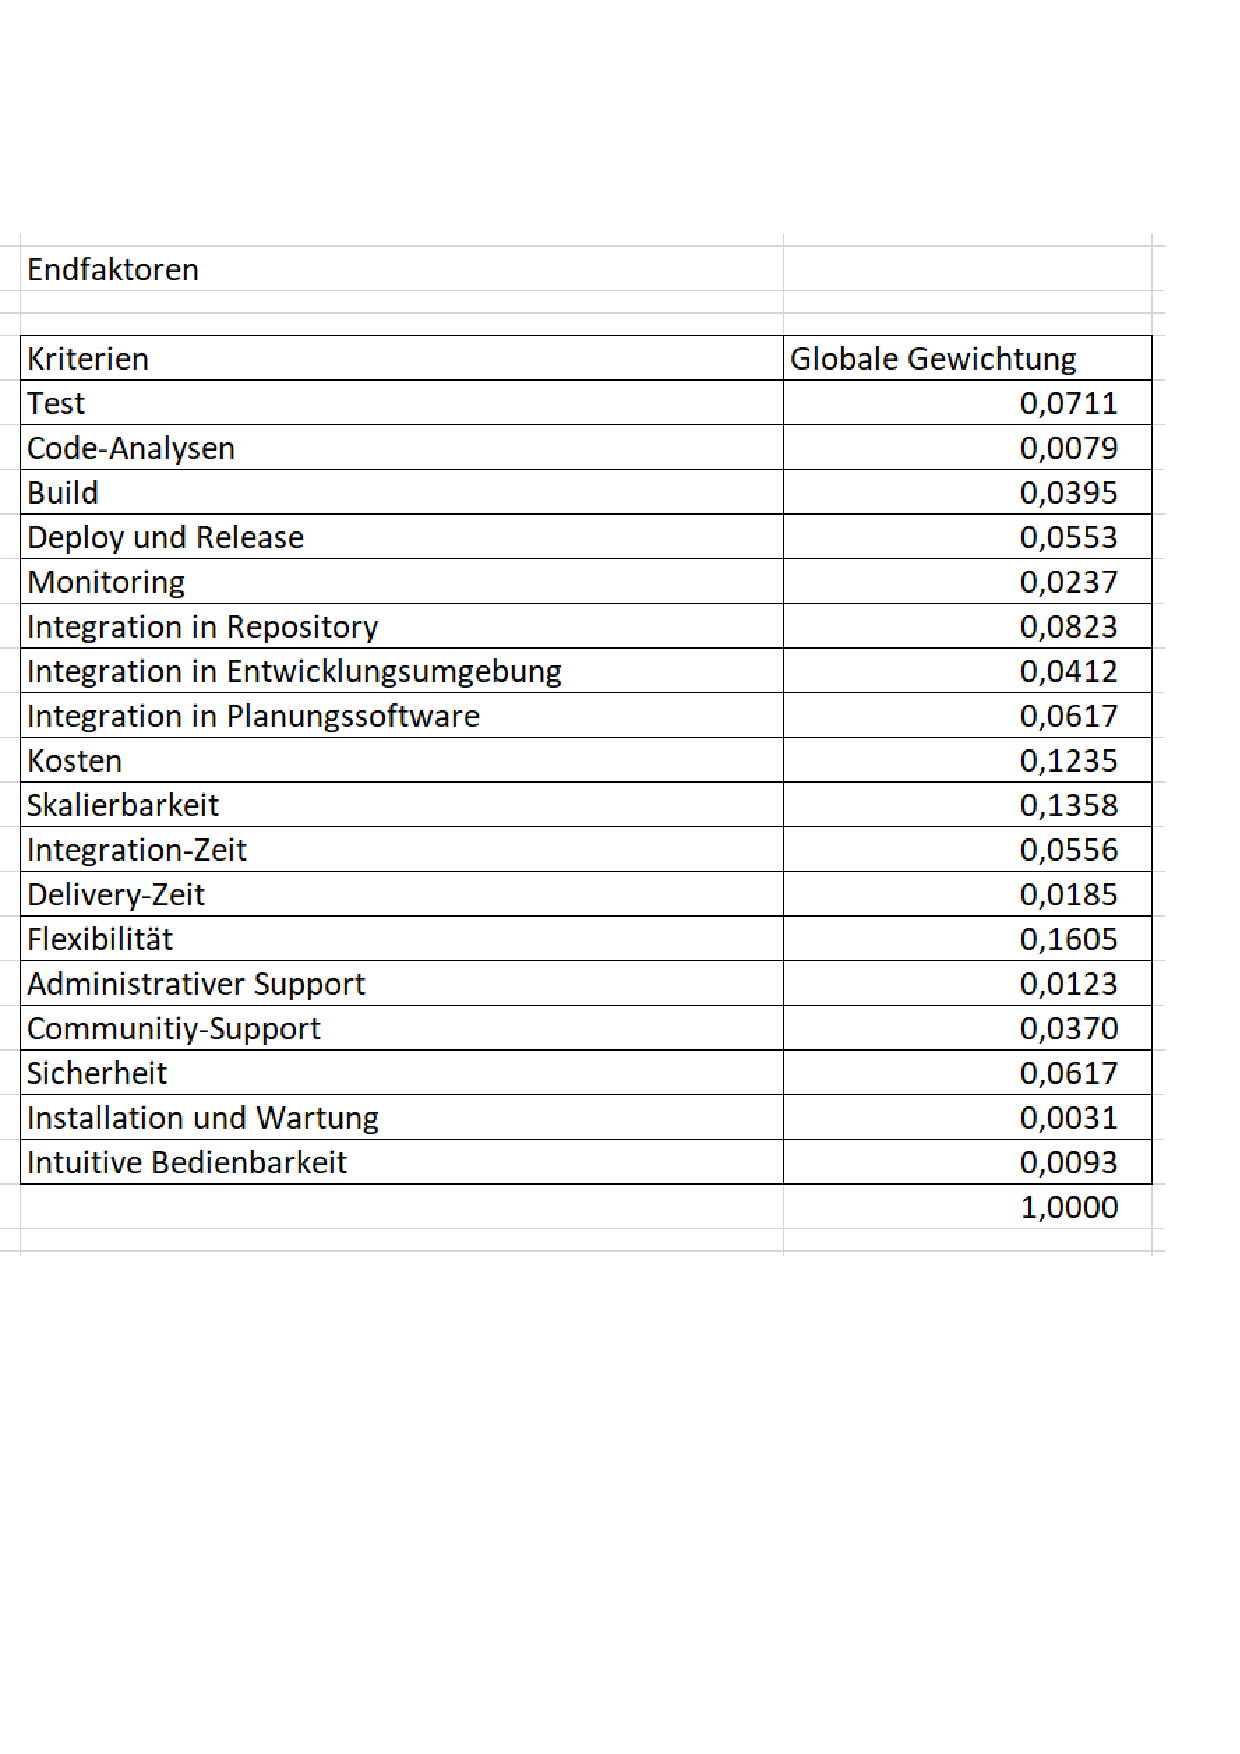
\includegraphics{Adams_3}}
    \label{fig:gew_43}
\end{figure}	
\end{center}
\newpage
\resetlinenumber
\begin{linenumbers}
    \textbf{Interviewer:} Fangen wir mit dem Subkriterium Funktionalität an. Kannst du deine Entscheidungen bitte begründen.\\
    \textbf{Experte:} Also für mich sind fast alle Funktionalitäten gleichgewichtig. Ich benötige alle diese Funktionalitäten, weil meine CI/CD-Pipeline sonst nicht sonderlich nützlich ist. Zu den Tests, der Hauptgrund der CI/CD-Pipeline ist es eigentlich Tests zu automatisieren. Ohne Build, Deploy und Release funktioniert meine Pipeline nicht. Ohne Monitoring kann ich nicht evaluieren, ob etwas fehlschlägt oder nicht. Code-Analysen sind hingegen bei Kundenprojekten oft nicht verpflichtend.\\
    \textbf{Interviewer:} Machen wir mit den Integrationsmöglichkeiten weiter. Für dich waren sowohl die Integration in das Repository als auch in eine Planungssoftware wichtig. Warum?\\
    \textbf{Experte:} Ich benötige auf jeden Fall mein Code für die Pipeline. Deswegen ist die Integration in das Repository eine essenzielle Funktionalität. Planungssoftware ist auch sehr wichtig, da das Business nicht in den Code reinschaut, sondern in eine Planungssoftware. In vielen Projekten, in den ich war, werden, die Ergebnisse der Code-Analysen unmittelbar in der Planungssoftware angezeigt.\\
    \textbf{Interviewer:} Für dich war die Integration-Zeit wichtiger als die Delivery-Zeit. Warum?\\
    \textbf{Experte:} Die Integration-Zeit ist sehr wichtig, um einen schnellen Feedback-Zyklus zu haben. Außerdem habe ich bereits in vielen Projekten gearbeitet, die ein Blue-Green-Deployment verwendet haben. So konnte nach Validierung lediglich auf eine neue Version umgeschaltet werden, wobei der Entwickler nicht durchgehend den Delivery-Prozess beobachten muss.\\ 
    \textbf{Interviewer:} Warum ist für dich sowohl der Community-Support als auch der administrative Support gleichgewichtig?\\
    \textbf{Experte:} Natürlich ist Community-Support sehr wichtig. Anderseits es natürlich auch sehr wichtig, dass eine gute Dokumentation und passende Schulungsunterlagen bereitstehen. \\
    \textbf{Interviewer:} Kannst du deine Entscheidung zur Benutzerfreundlichkeit begründen?\\
    \textbf{Experte:} Eigentlich ist es so, dass man ein Pipeline-System einmal aufsetzt und dieses dann nicht mehr sonderlich viel Konfiguration benötigt. Was i.d.R. häufiger gemacht wird, insbesondere in einer Composable-Enterprise-Architektur ist das Aufsetzen von Pipelines. Deshalb ist die intuitive Bedienbarkeit einfach sehr wichtig.\\
    \textbf{Interviewer:} Noch einmal zu den Kriterien auf oberster Ebene. Warum sind dir Sicherheit und Funktionalität so wichtig?\\
    \textbf{Experte:} Das Bereitstellen von Software schöpft Wert für das Unternehmen. Deswegen ist es einfach wichtig, dass keiner in meine Pipelines eingreifen kann und diesen Prozess stören kann. Funktionalität ist natürlich essenziell, dass mein Pipeline-System auch das abdecken kann, was dann letztendlich benötigt wird.\\
    
\end{linenumbers}


\newpage
\subsection{Expertengewichtung 5}
        \begin{tabular}{ l l }
    Interviewpartner: & Product Manager SAP CLM (Experte 8)\\
    Datum: & 22.03.2023\\
    Interview-Medium: & Microsoft-Teams\\
\end{tabular}
\begin{center}
\begin{figure}[H]
    \centering
    \scalebox{0.6}{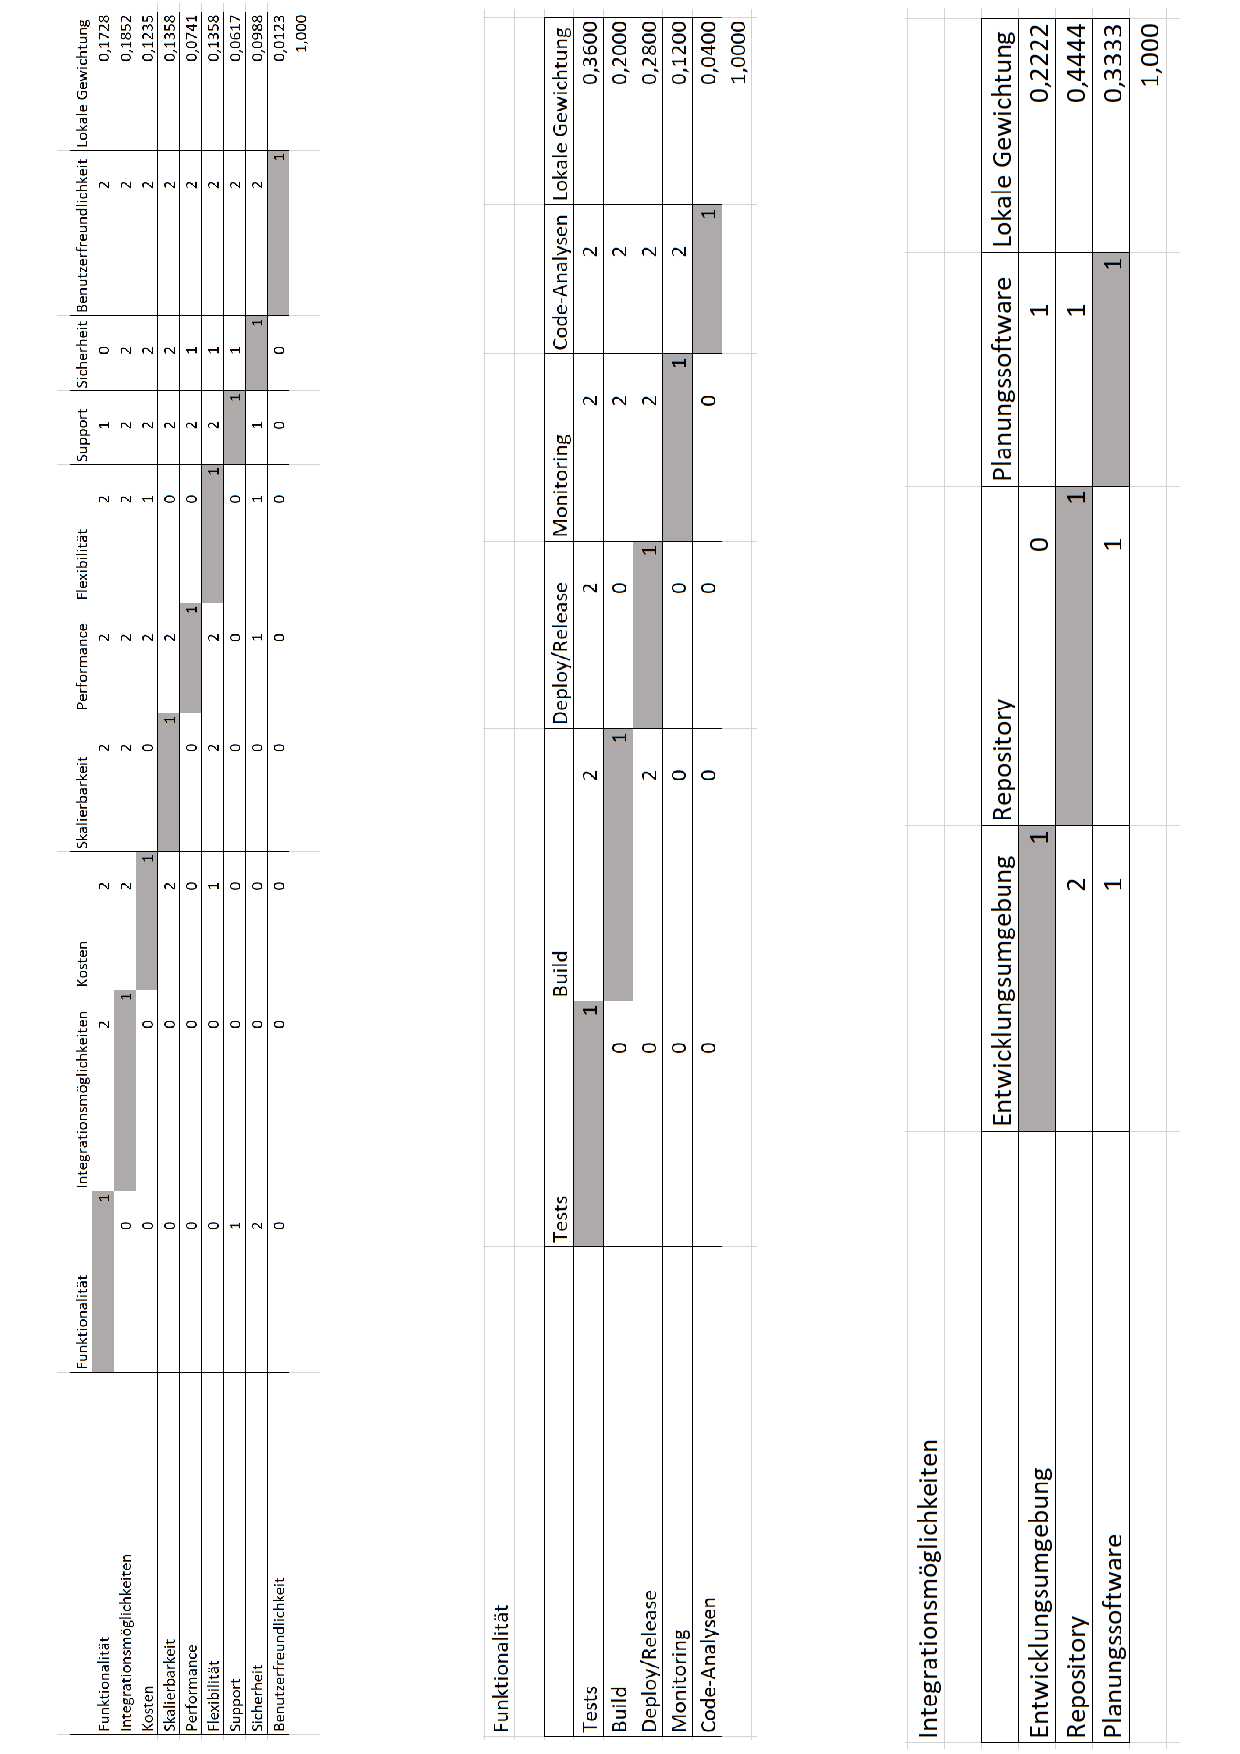
\includegraphics{Zarske_1}}
    \label{fig:gew_51}
\end{figure}	
\end{center}
\begin{center}
\begin{figure}[H]
    \centering
    \scalebox{0.7}{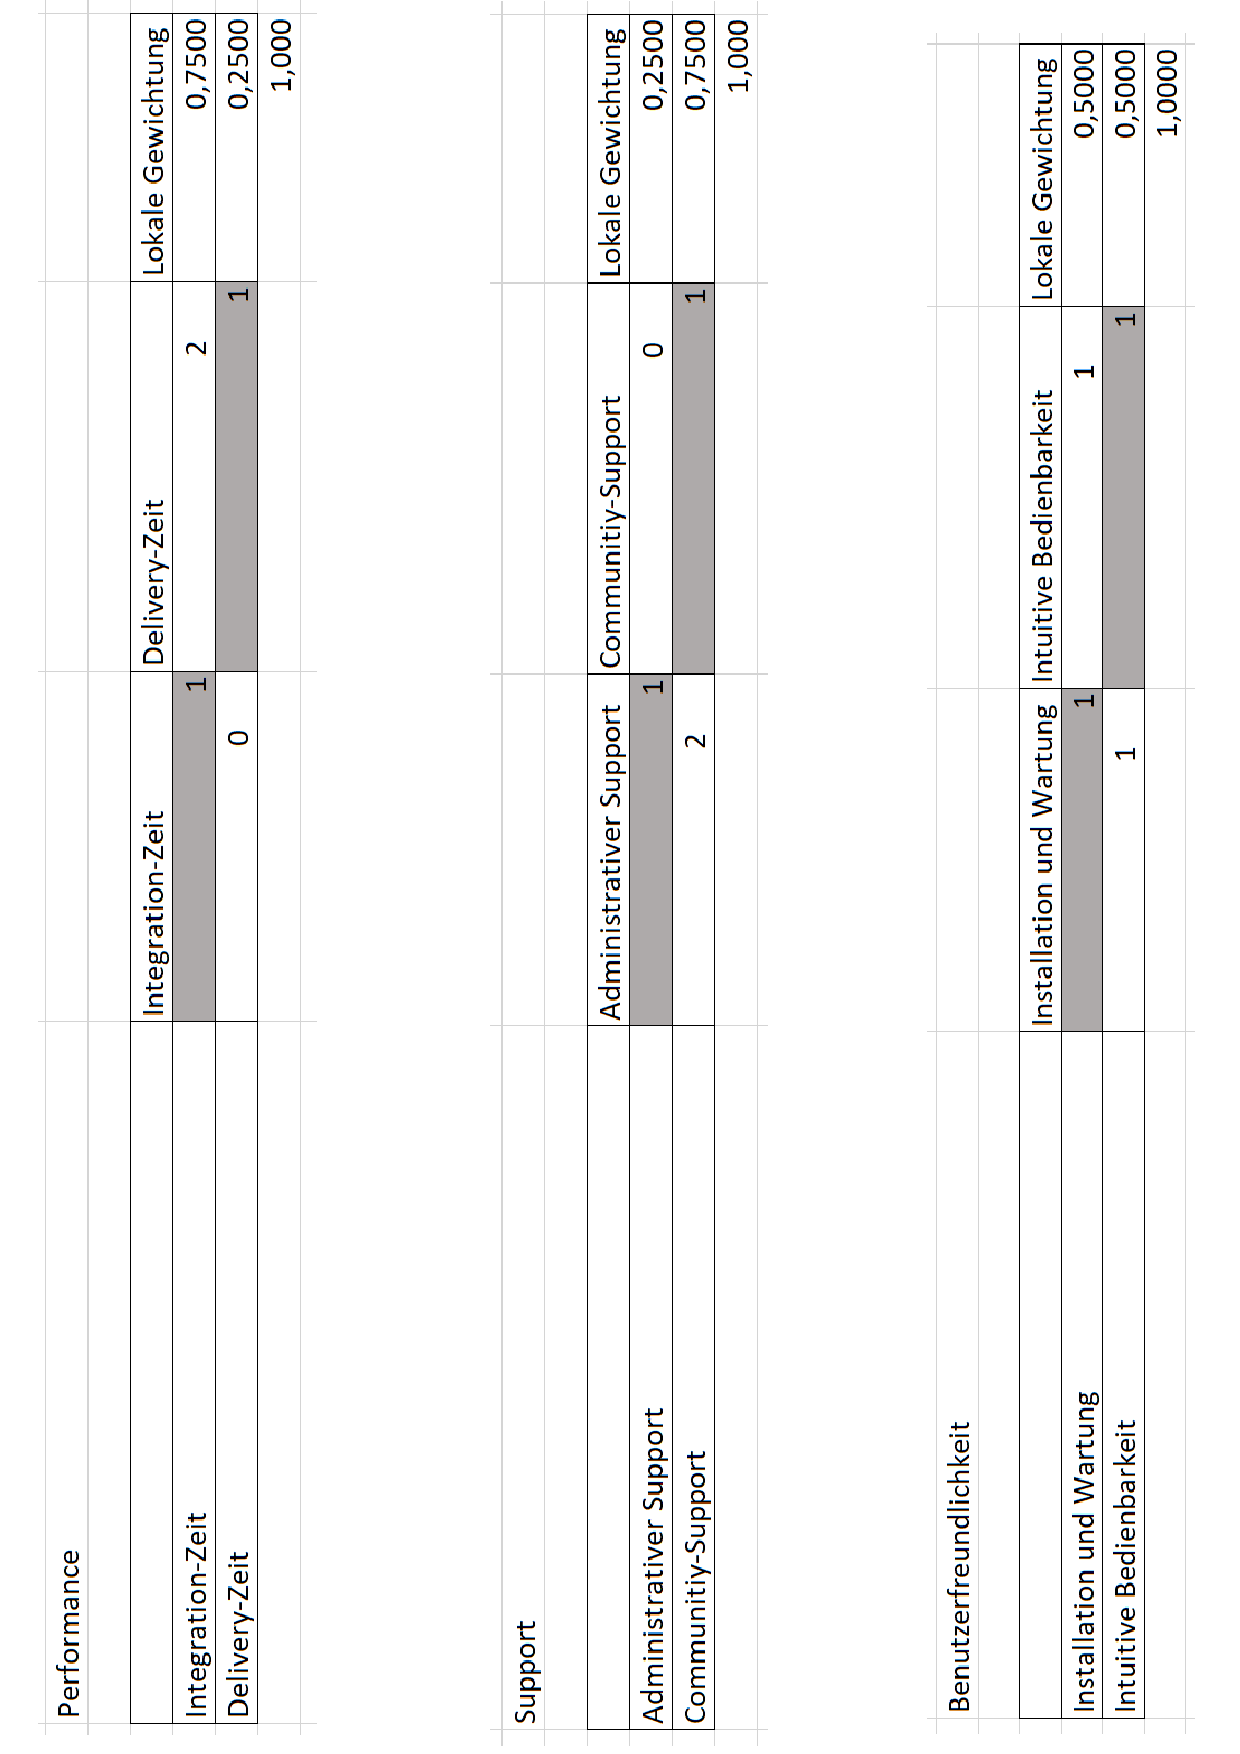
\includegraphics{Zarske_2}}
    \label{fig:gew_52}
\end{figure}	
\end{center}

\begin{center}
\begin{figure}[H]
    \centering
    \scalebox{0.7}{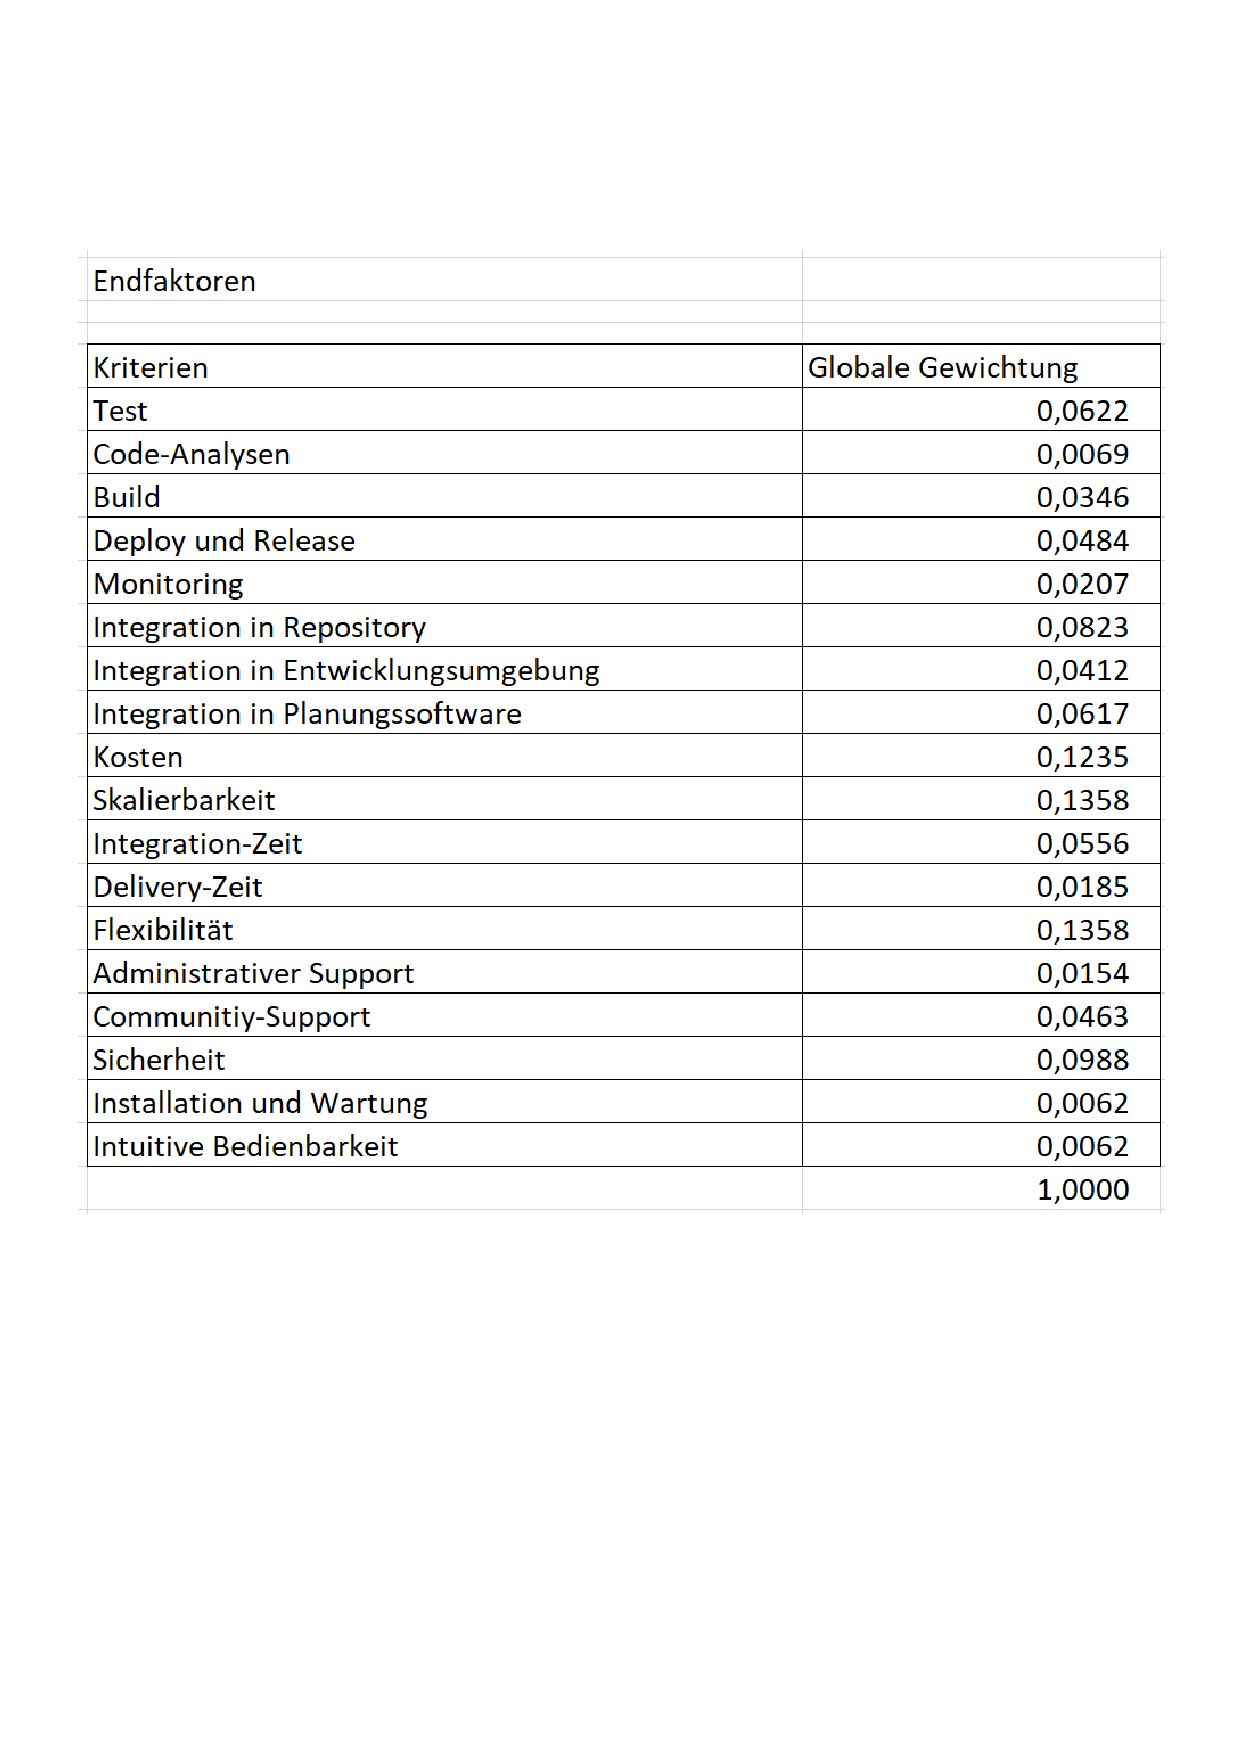
\includegraphics{Zarske_3}}
    \label{fig:gew_53}
\end{figure}	
\end{center}
\newpage
\resetlinenumber
\begin{linenumbers}
    \textbf{Interviewer:} Fangen wir auf oberster Ebene an. Besonders wichtig war für dich die Integration. Warum?\\
    \textbf{Experte:} Kunden wollen insbesondere, dass die CI/CD-Tools in ihre Prozesse integrierbar sind. Da spielt es natürlich eine sehr große Rolle, welches Repository diese verwenden. Sicherheit kann dann natürlich auch ein K.O.-Kriterium sein. Wenn keine angemessenen Sicherheitsrichtlinien vorhanden sind, kann das natürlich ein Grund sein eine Pipeline nicht zu wählen. \\
    \textbf{Interviewer:} Machen wir mit dem Subkriterium Funktionalität weiter.\\
    \textbf{Experte:} Der Build war für mich sehr wichtig. Das liegt einfach daran, dass man ohne den Build gar nicht erst weiter kommt. Natürlich ist der Hauptgrund von CI/CD-Pipelines automatisierte Tests durchzuführen, jedoch funktioniert das ohne den Build erst gar nicht. Es gibt einige Kunden, die auch ganz stark auf Compliance achten, weswegen Code-Analysen schon auch gleichwertig wie die Test-Funktionalität ist. Was Deploy und Release angeht, es gibt auch einige Kunden, die auch darauf verzichten.\\
    \textbf{Interviewer:} Kommen wir zur Integration. Für dich ist die Integration in das Repository sehr wichtig. Warum?\\
    \textbf{Experte:} Das gehört meiner Meinung nach zur Voraussetzung. Was die Planungssoftware angeht, haben die Kunden meistens isolierte Lösungen.\\ 
    \textbf{Interviewer:} In der Kategorie der Performance war dir die Integration-Zeit wichtiger. Warum?\\
    \textbf{Experte:} Meiner Erfahrung nach war es für die Kunden oft in Ordnung, wenn die Delivery-Zeit ein wenig länger dauert. Das liegt auch daran, dass vor dem Deploy noch oft manuelle Schritte gemacht werden.\\
    \textbf{Interviewer:} Kannst du deine Entscheidung zum Support begründen?\\
    \textbf{Experte:} Ich habe den administrativen Support höher gewertet, da ich die Erfahrung gemacht habe, dass Kunden sehr viel Wert auf die SLAs legen. So weiß der Kunde natürlich genau, dass er sich auch am Wochenende melden kann, wenn er ein Problem hat und dann auch entsprechend eine Antwort bekommt. \\
    \textbf{Interviewer:} Kannst du auch noch deine Entscheidung zur Benutzerfreundlichkeit begründen.\\
    \textbf{Experte:} Ich habe die Intuitive Bedienbarkeit sowie Installation und Wartung auf eine Wichtigkeitsstufe gesetzt. Zum einen ist es natürlich so, dass die intuitive Bedienbarkeit etwas ist, mit welchem man alltäglich zu tun hat. Aber gerade bezüglich des Wartens von komplexen Infrastrukturen, war es für viele Kunden der Grund sich dann letztendlich für eine SaaS-Lösung zu entscheiden.\\
\end{linenumbers}



\newpage
\subsection{Expertengewichtung Durchschnitt}
\begin{center}
\begin{figure}[H]
    \centering
    \scalebox{0.6}{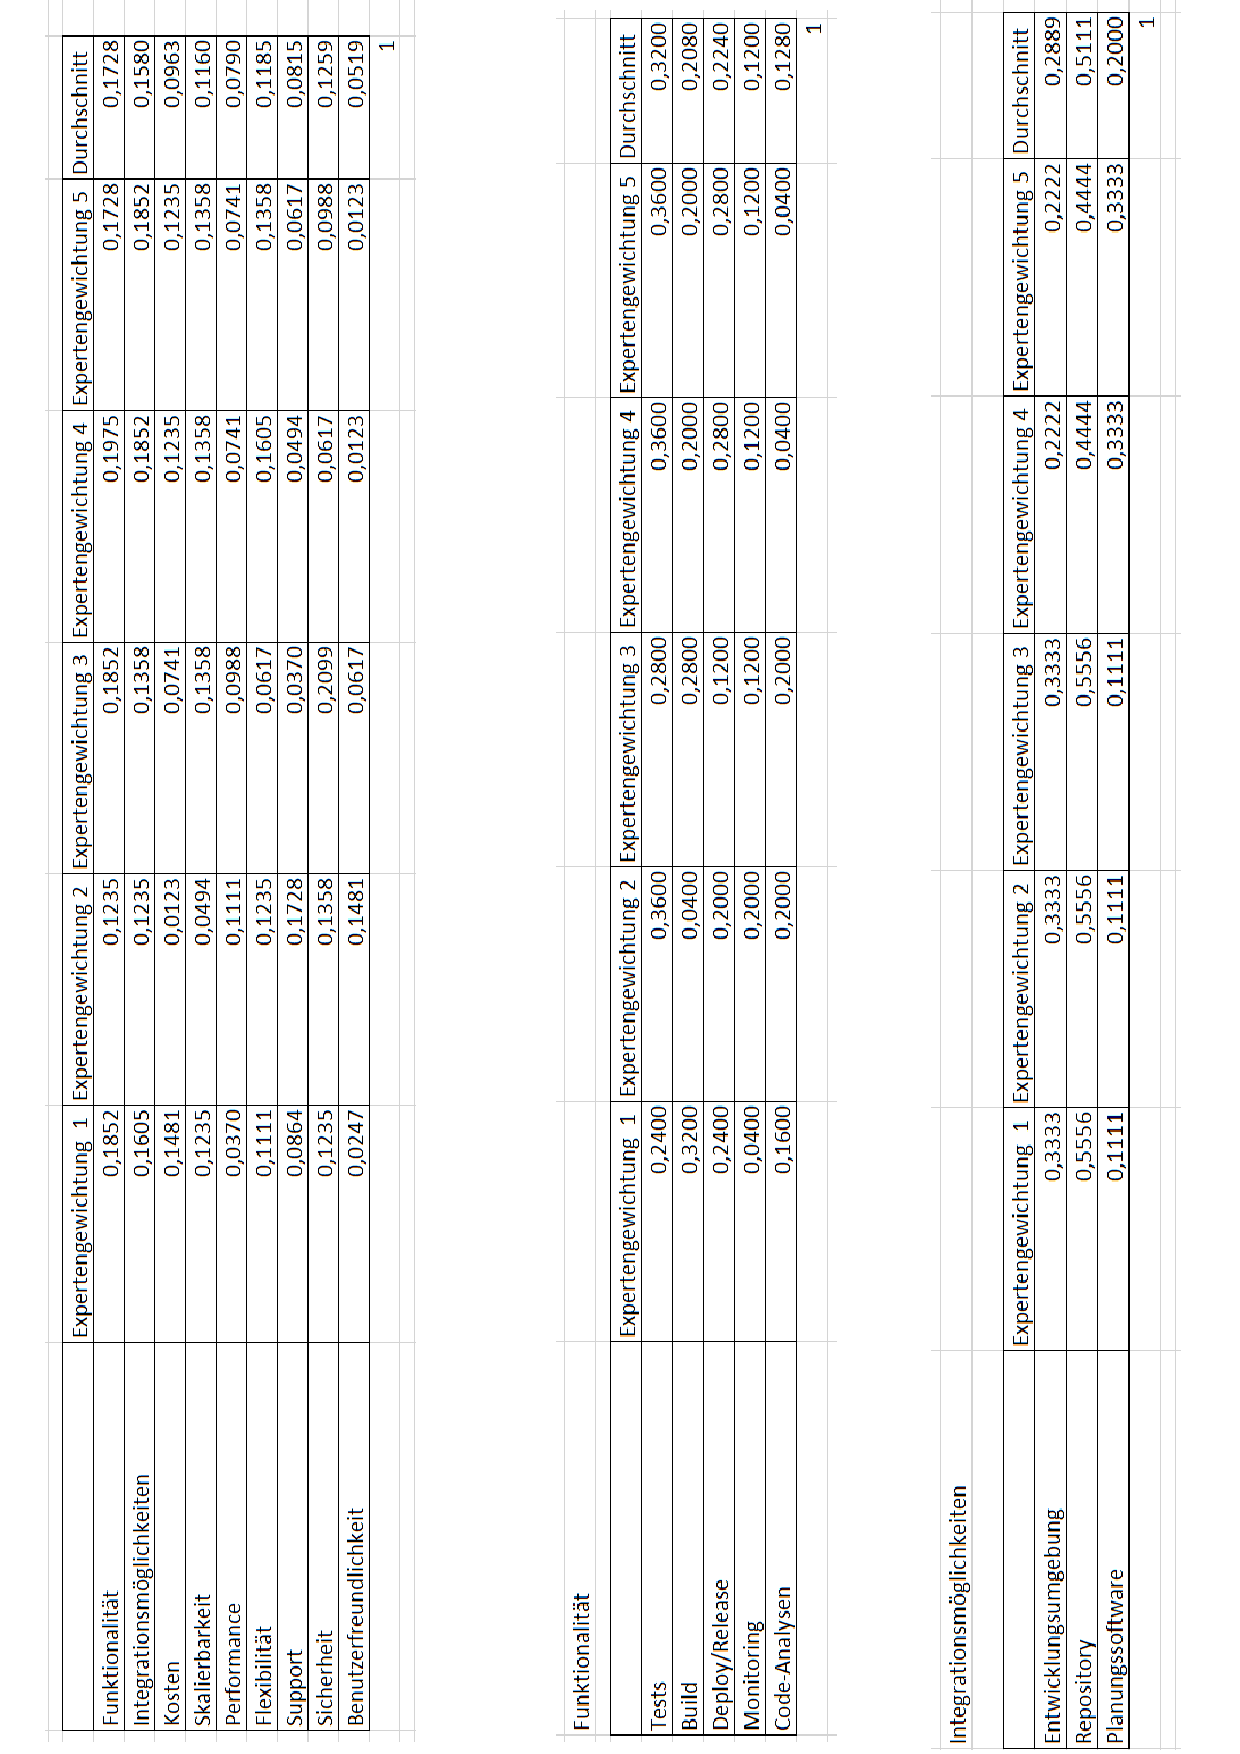
\includegraphics{Durchschnitt_1}}
    \label{fig:gew_d1}
\end{figure}	
\end{center}
\begin{center}
\begin{figure}[H]
    \centering
    \scalebox{0.7}{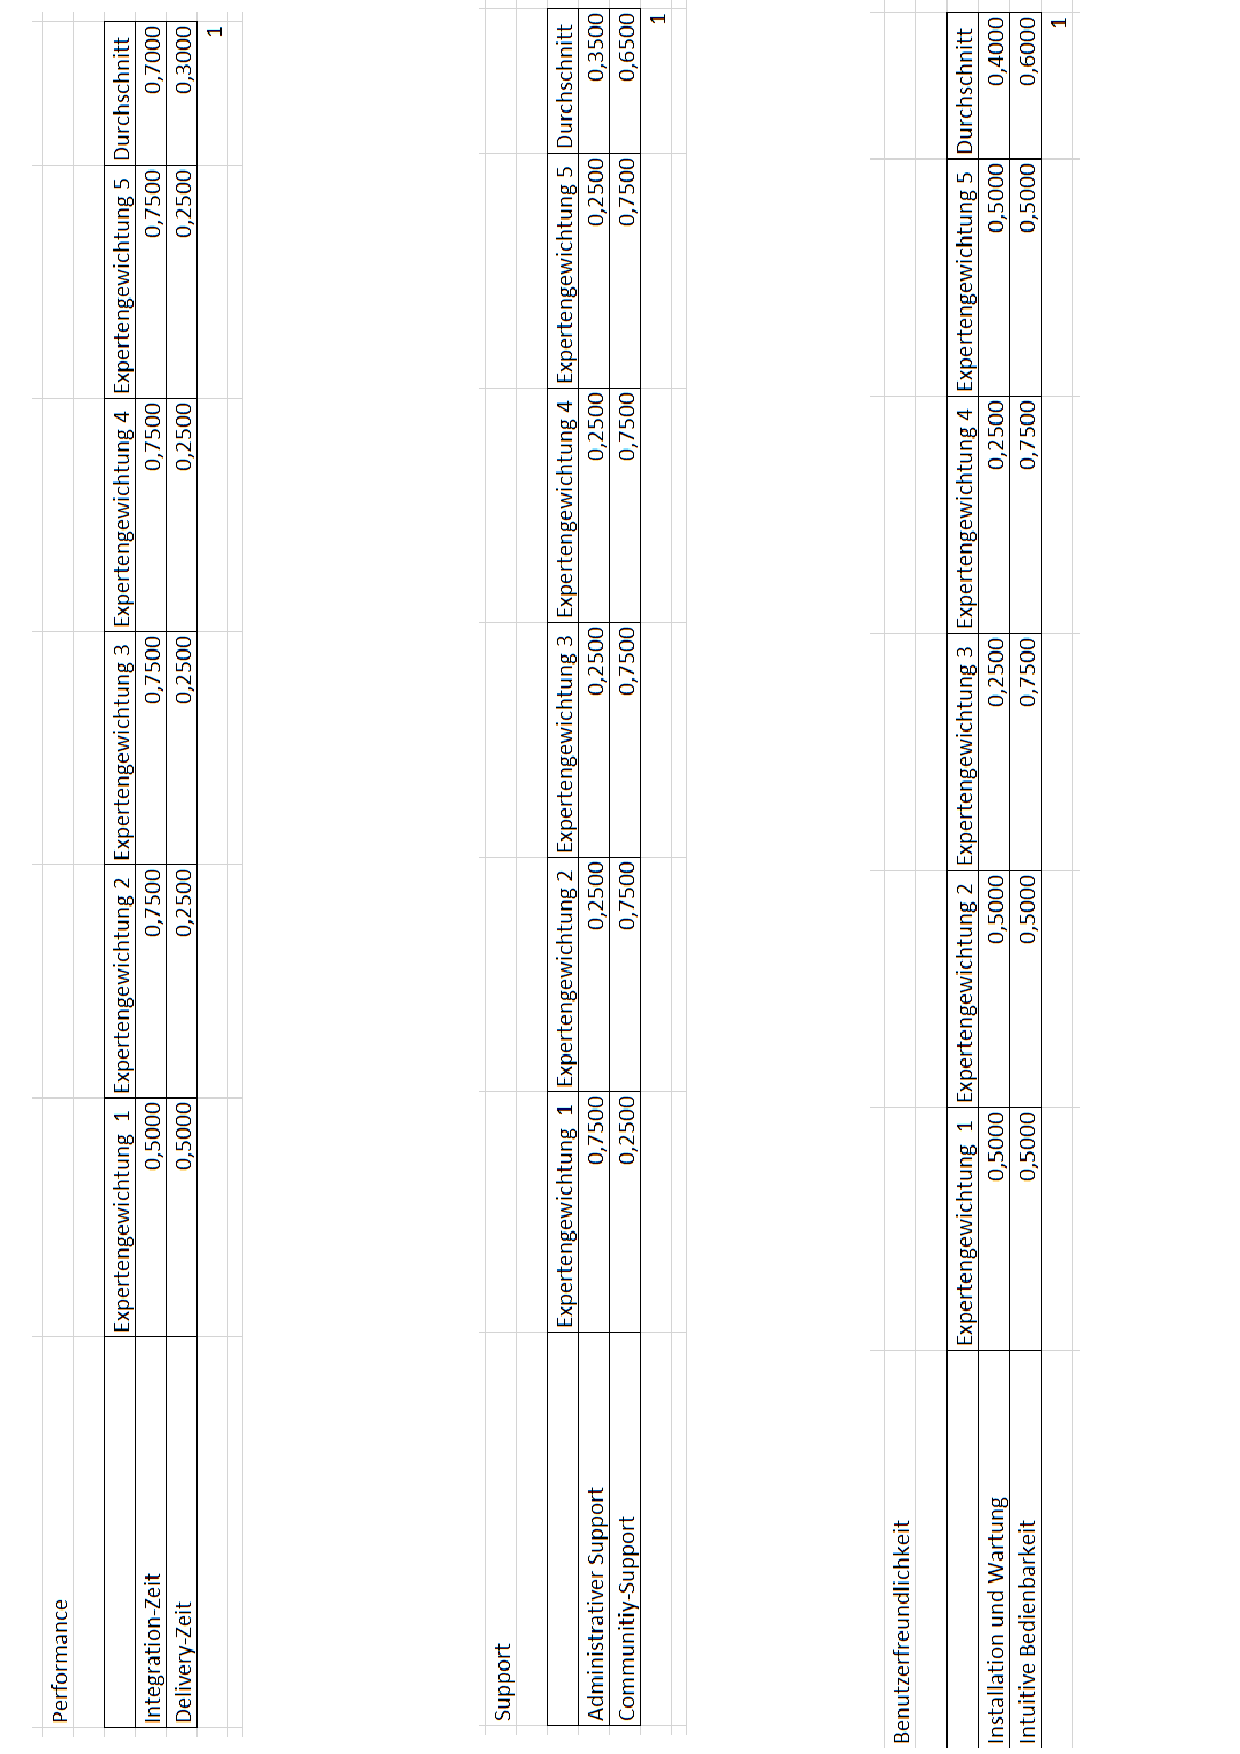
\includegraphics{Durchschnitt_2}}
    \label{fig:gew_d2}
\end{figure}	
\end{center}

\begin{center}
\begin{figure}[H]
    \centering
    \scalebox{0.7}{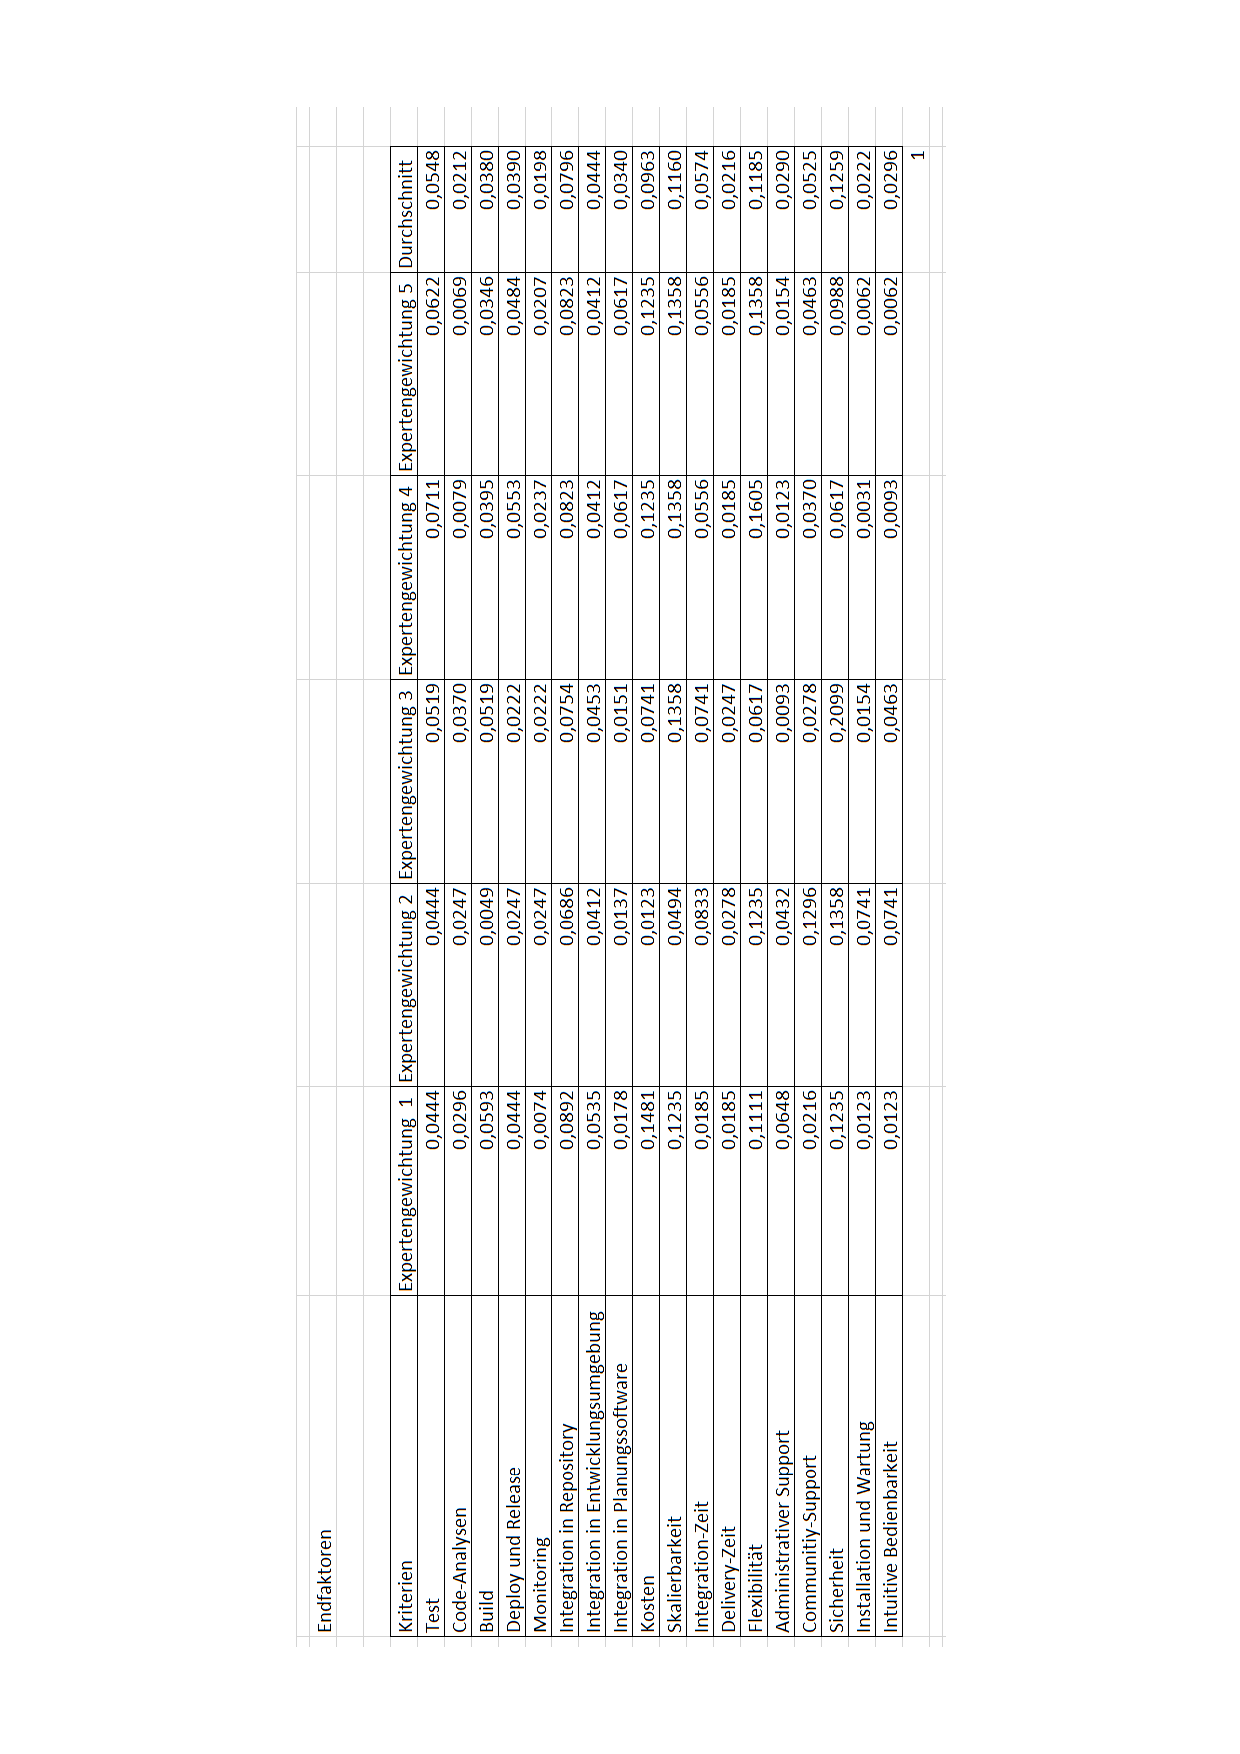
\includegraphics{Durchschnitt_3}}
    \label{fig:gew_d3}
\end{figure}	
\end{center}